\documentclass[a4paper,11pt]{amsbook}

\usepackage{pdfpages}
\usepackage{hyperref}
\usepackage[margin=1in]{geometry}
% \usepackage{tocloft}
% \renewcommand{\cftpartleader}{\cftdotfill{\cftdotsep}} % for parts
% \renewcommand{\cftchapleader}{\cftdotfill{\cftdotsep}} % for chapters

\title{Level Three Calculus\\Worksheets}
\author{Alexander Elzenaar}
\date{\today}

\begin{document}

  \begin{titlepage}
    \centering

    \vspace*{\fill}

    \makeatletter

    \Huge{\textbf{\@title}}

    \vspace*{2cm}

    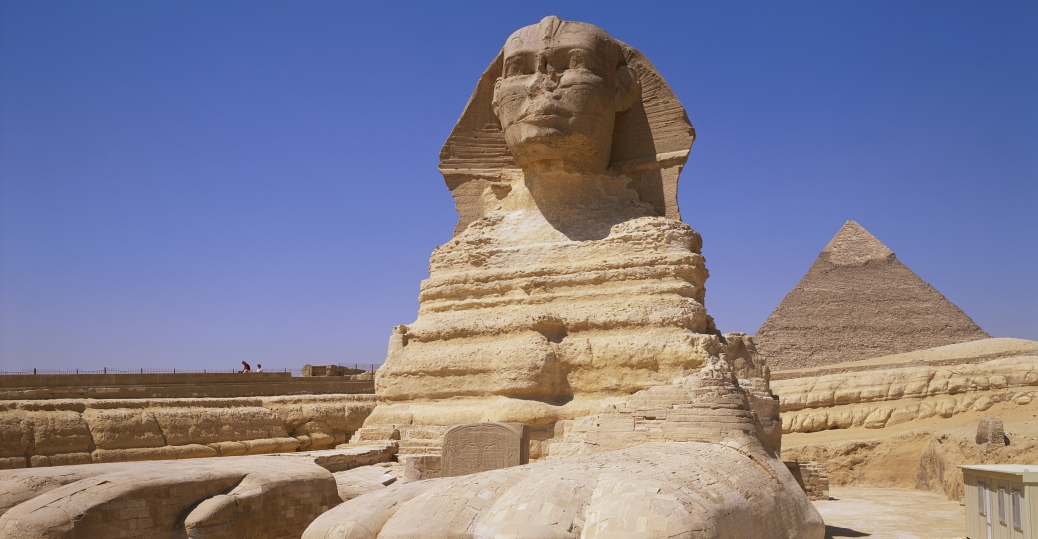
\includegraphics[width=0.9\textwidth]{bookcover}

    \vspace*{2cm}

    \Large\textit{\authors}

    \vspace*{\fill}

    \makeatother
  \end{titlepage}

  \tableofcontents

  \chapter{Preamble}
  \phantomsection\addcontentsline{toc}{section}{Introduction to the Notes}
  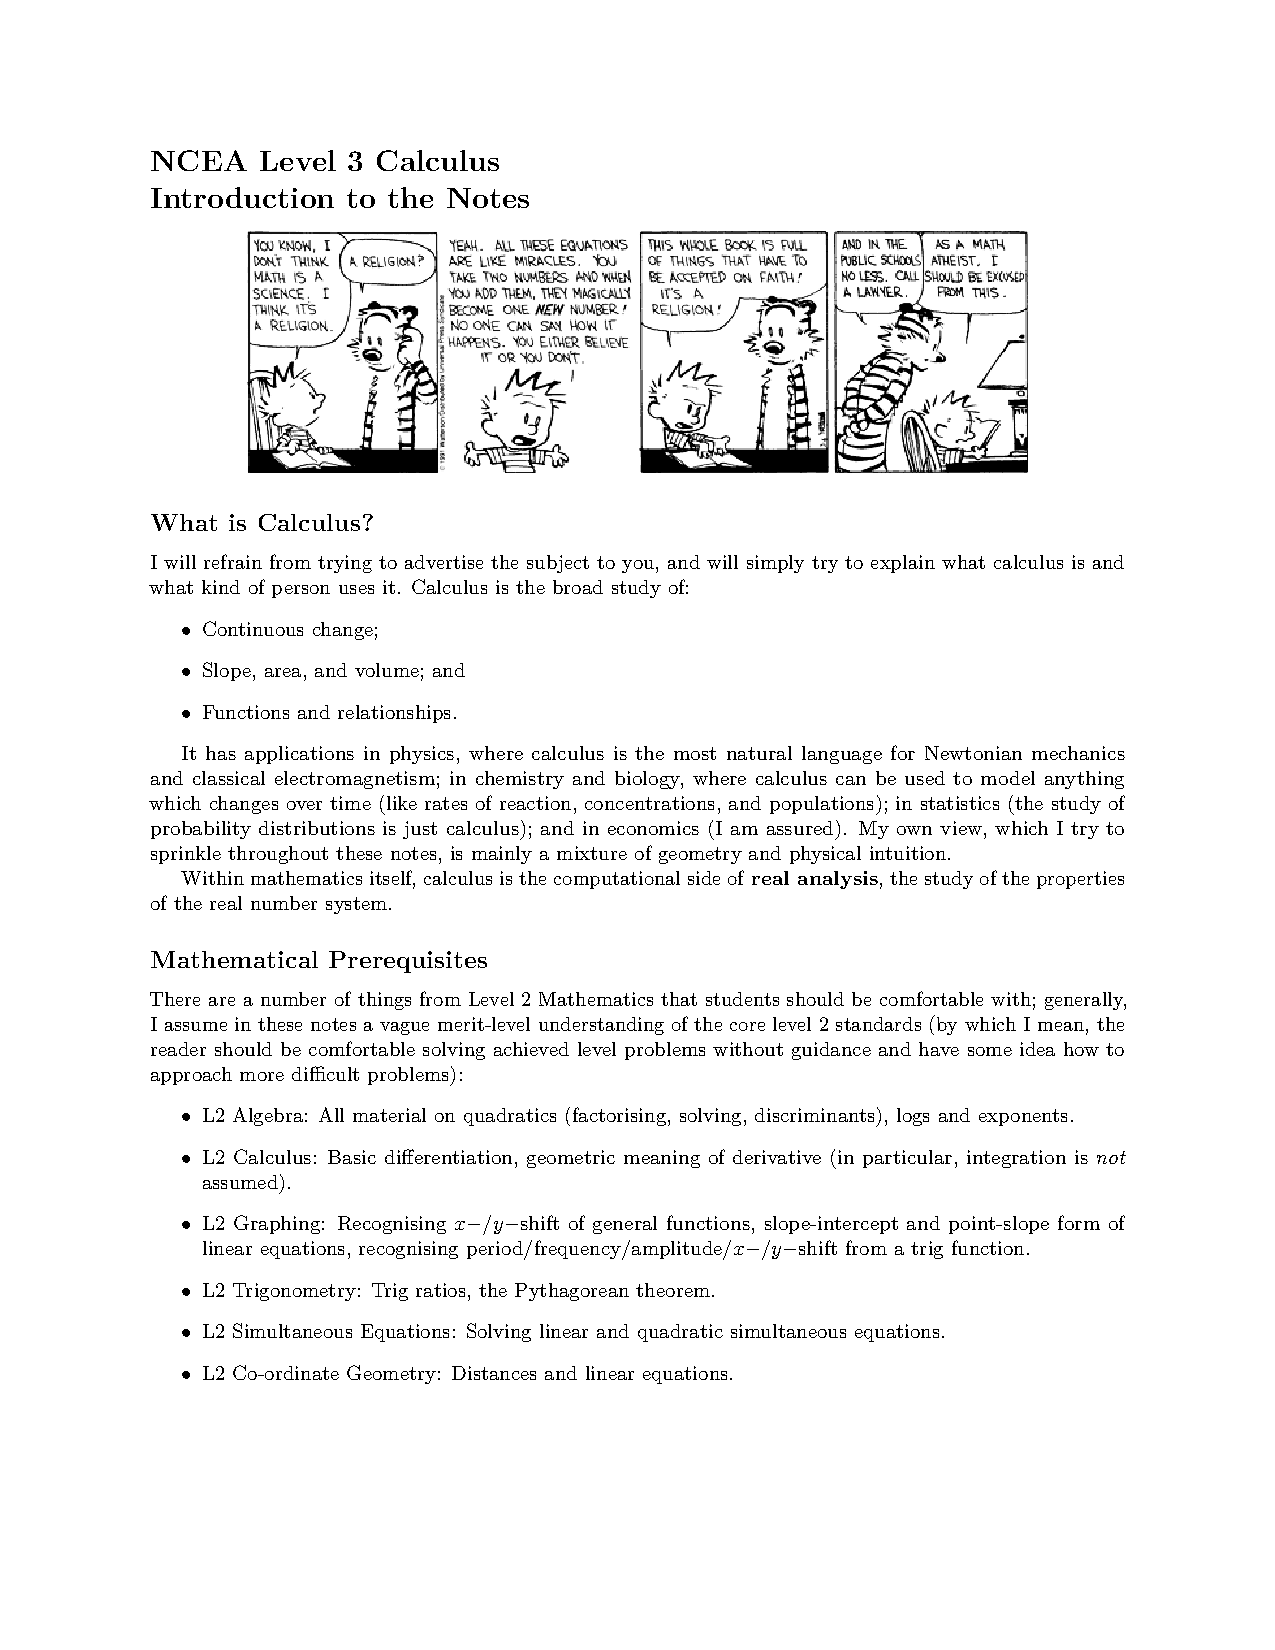
\includepdf[pages={-},pagecommand={}]{00-introduction.pdf}
  \phantomsection\addcontentsline{toc}{section}{Prior Revision: Functions}
  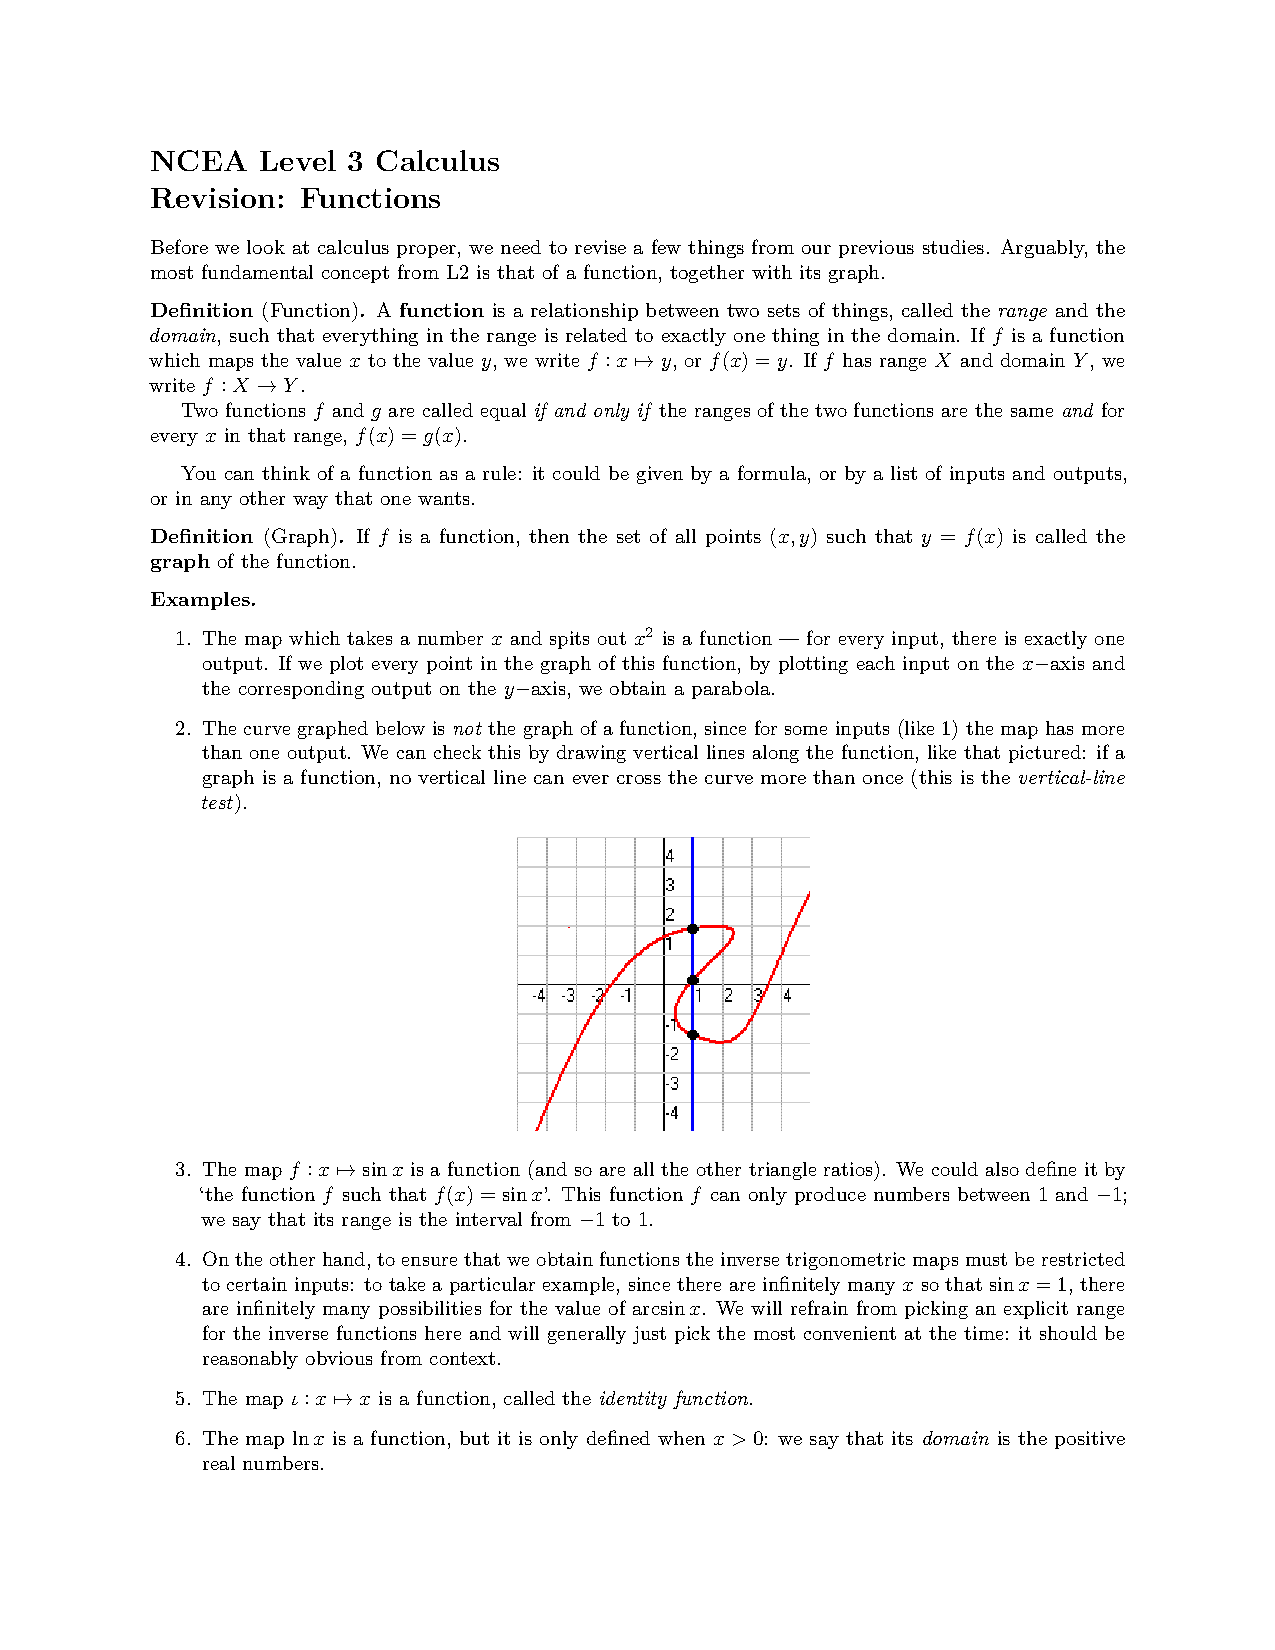
\includepdf[pages={-},pagecommand={}]{RV-functions.pdf}

  \chapter{Differentiation}
  \phantomsection\addcontentsline{toc}{section}{1. The Derivative}
  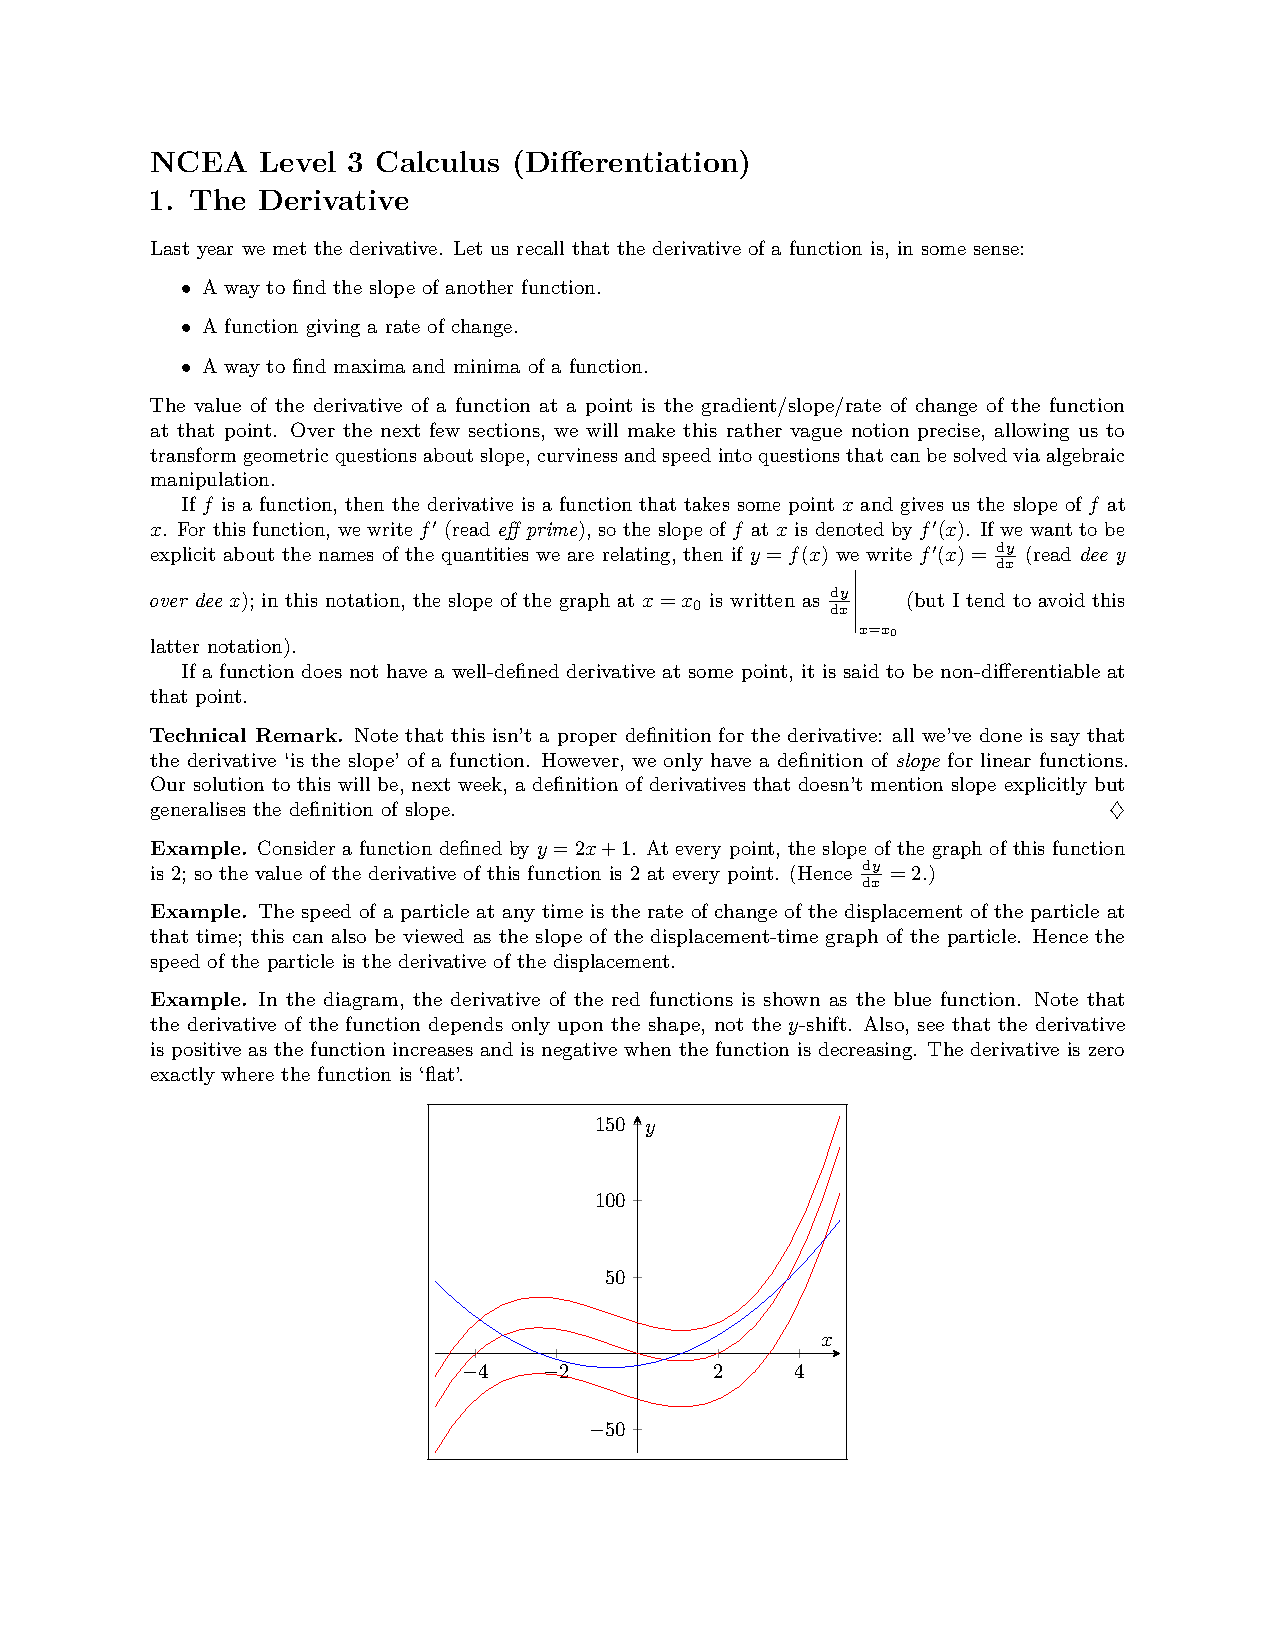
\includepdf[pages={-},pagecommand={}]{01-geometric.pdf}
  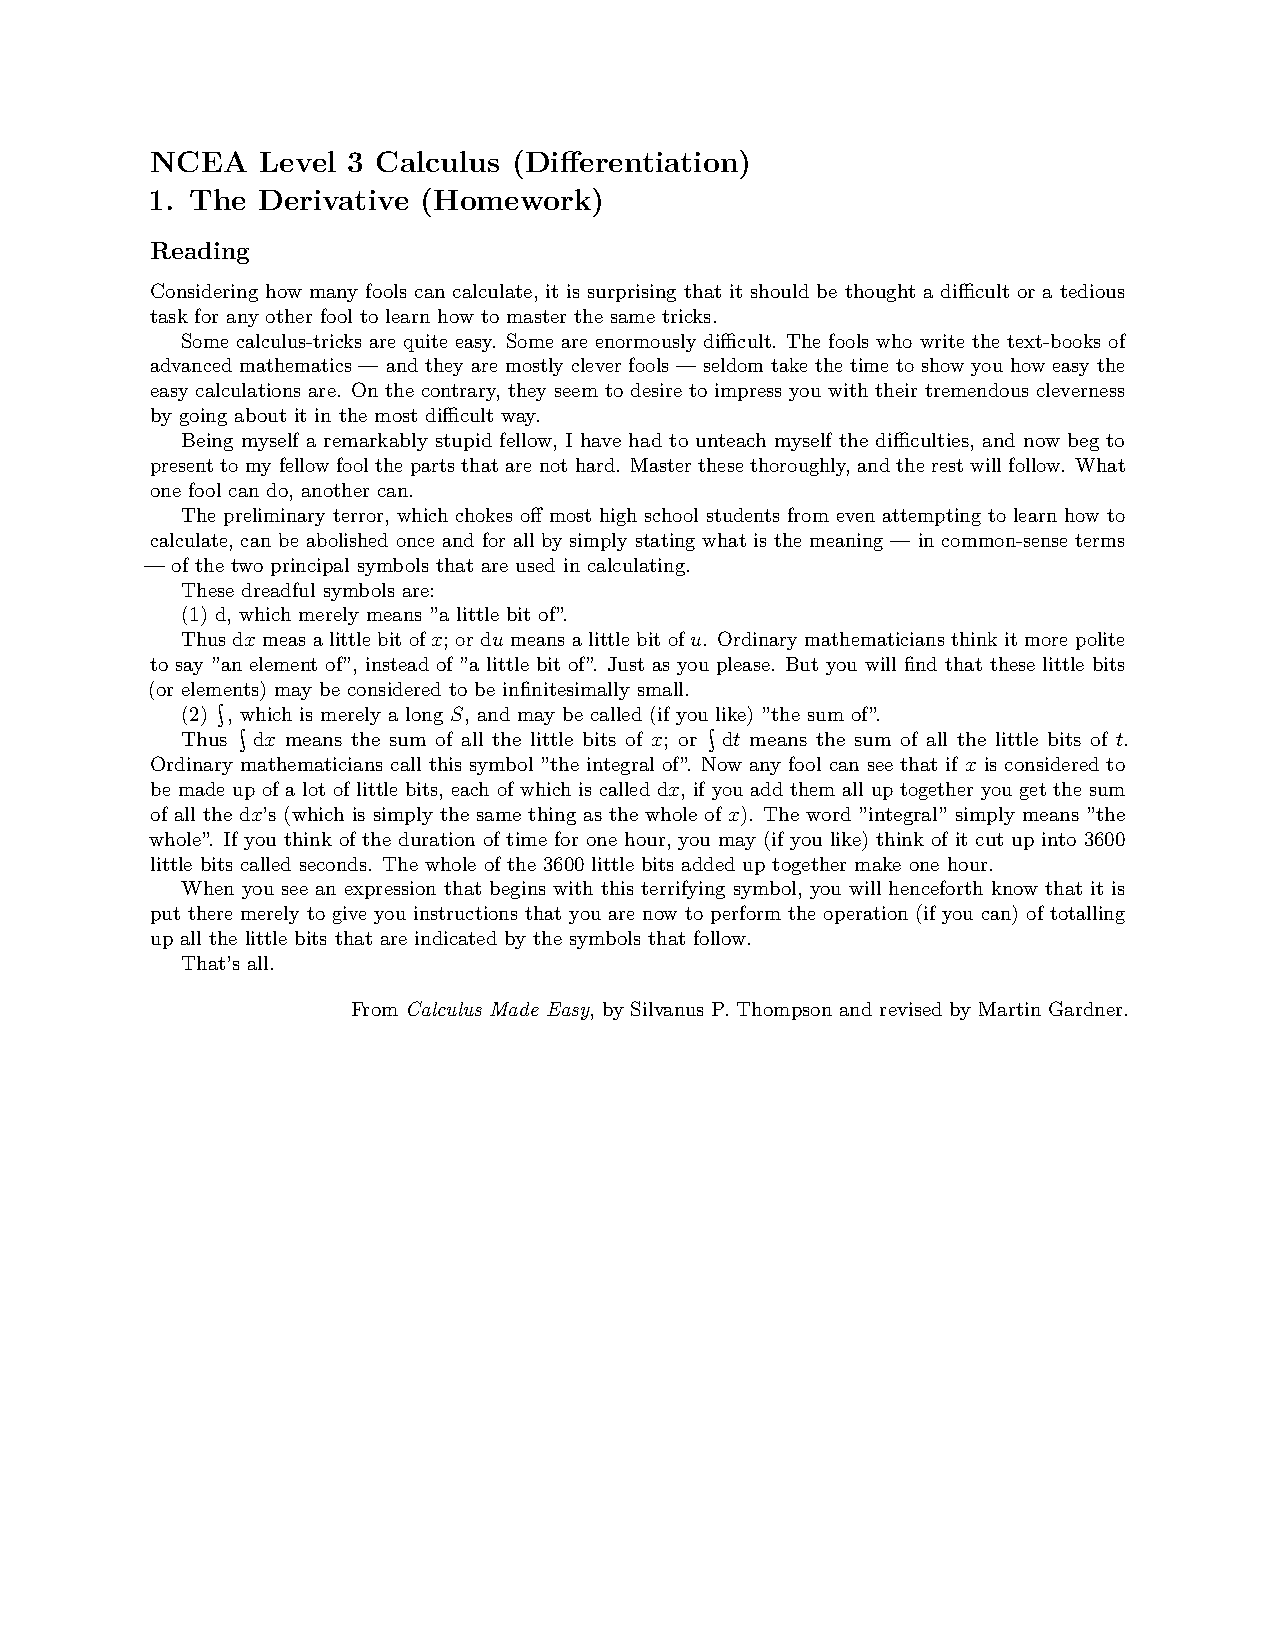
\includepdf[pages={-},pagecommand={}]{01-geometric-hw.pdf}
  \phantomsection\addcontentsline{toc}{section}{2. Limits}
  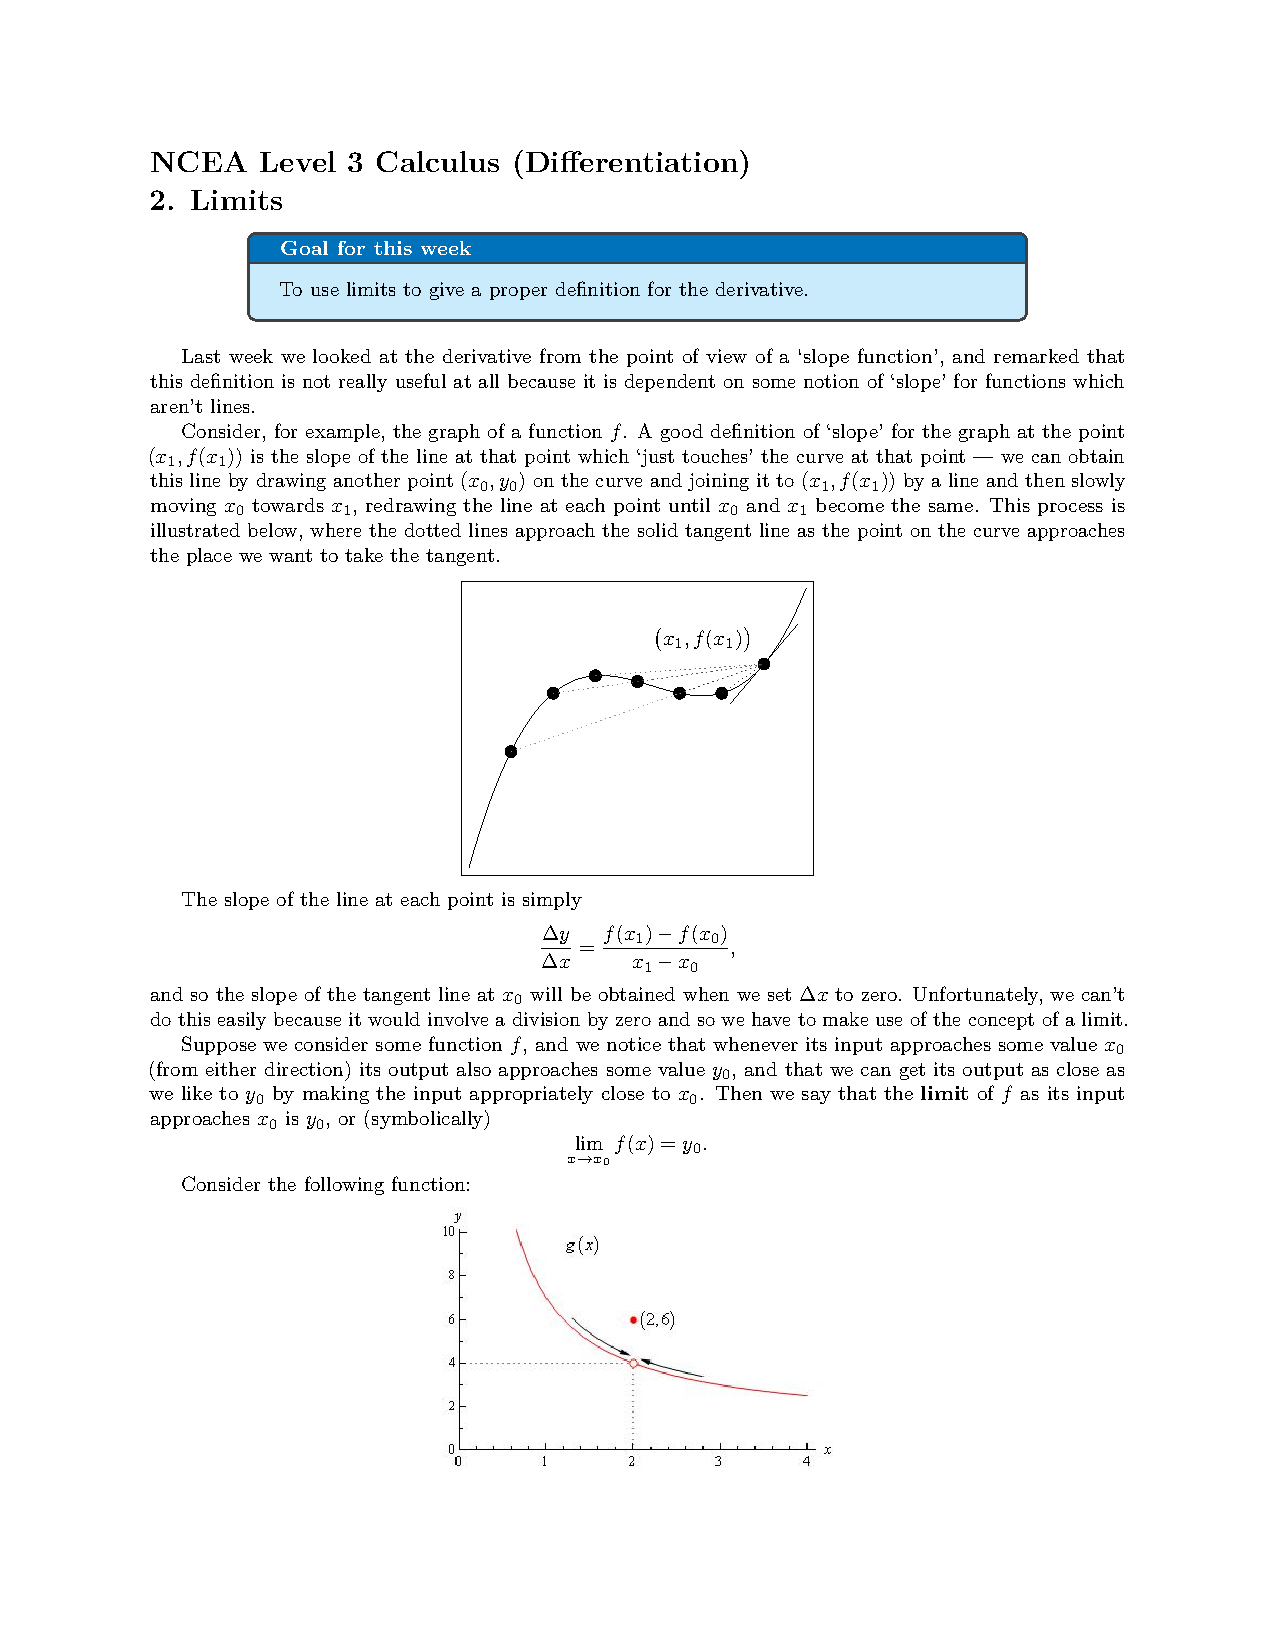
\includepdf[pages={-},pagecommand={}]{02-limits.pdf}
  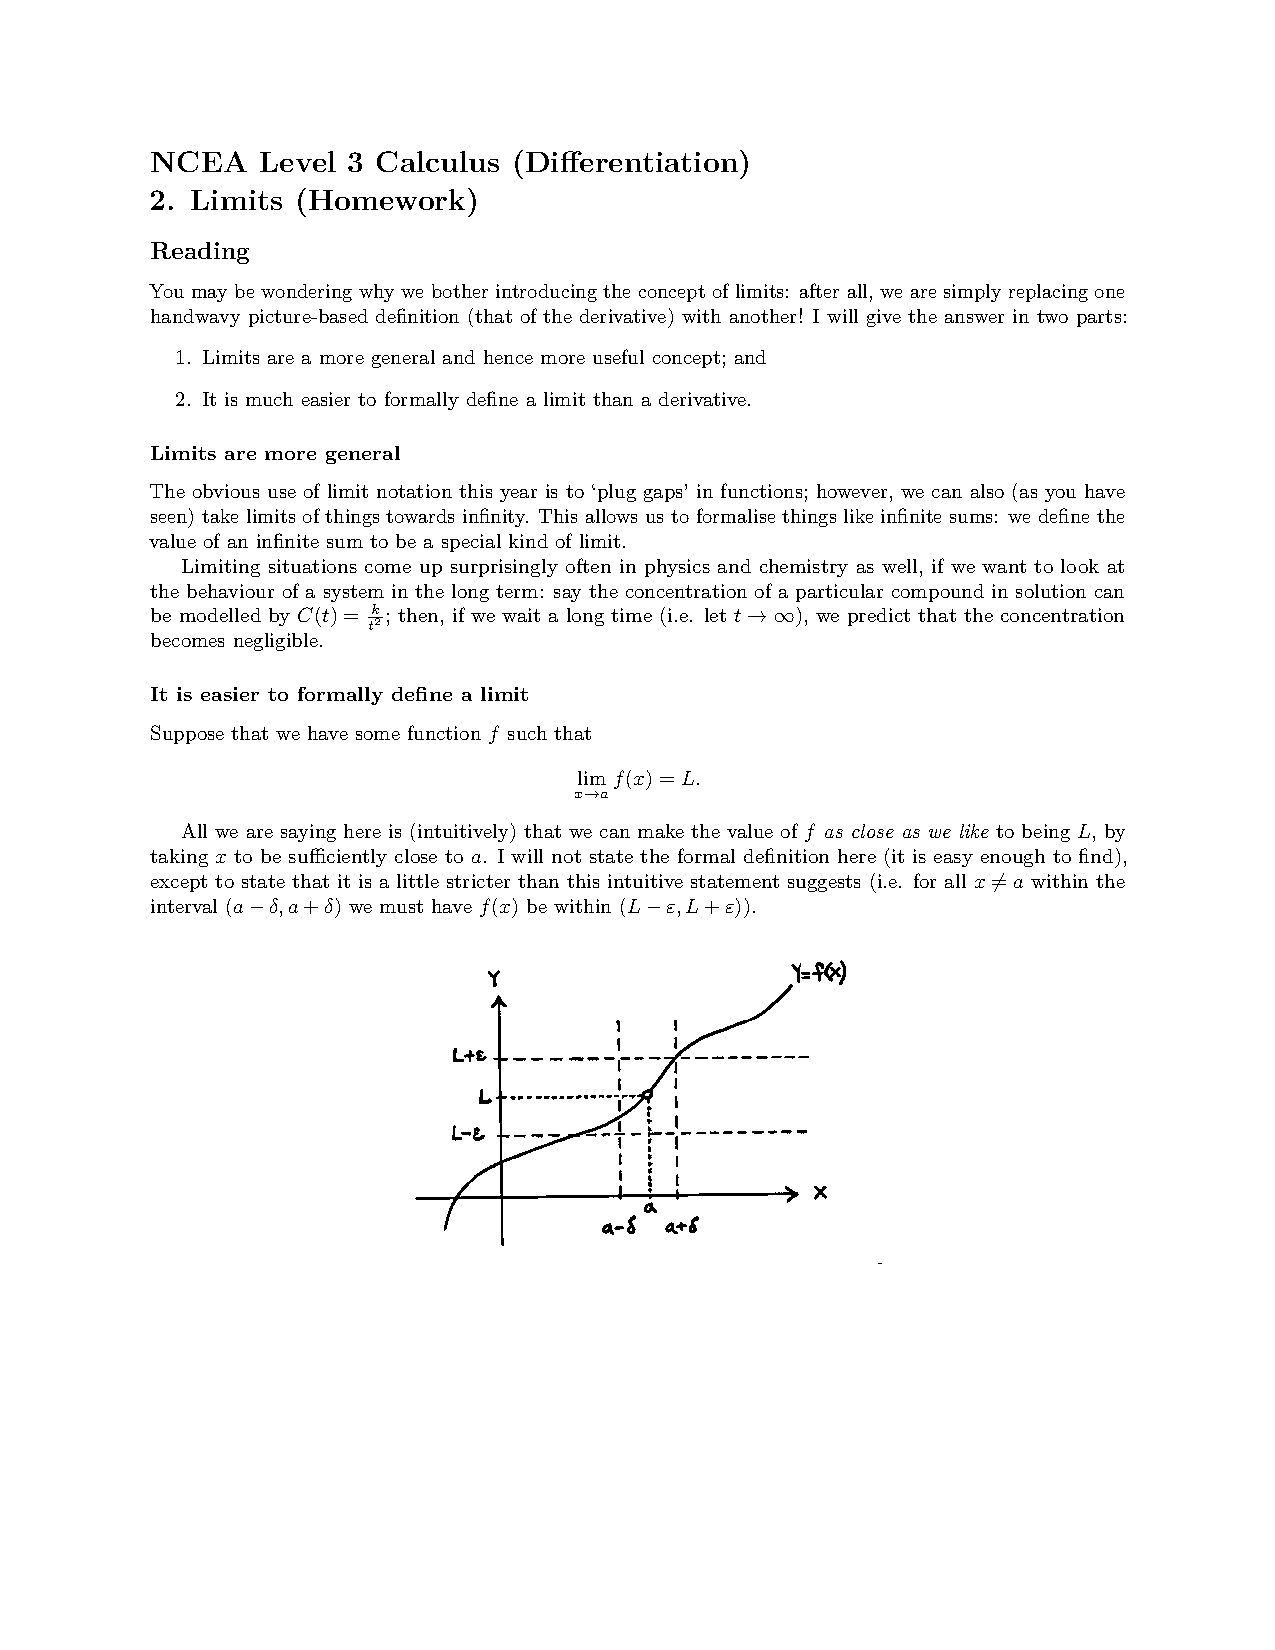
\includepdf[pages={-},pagecommand={}]{02-limits-hw.pdf}
  \phantomsection\addcontentsline{toc}{section}{3. Derivatives of Common Functions}
  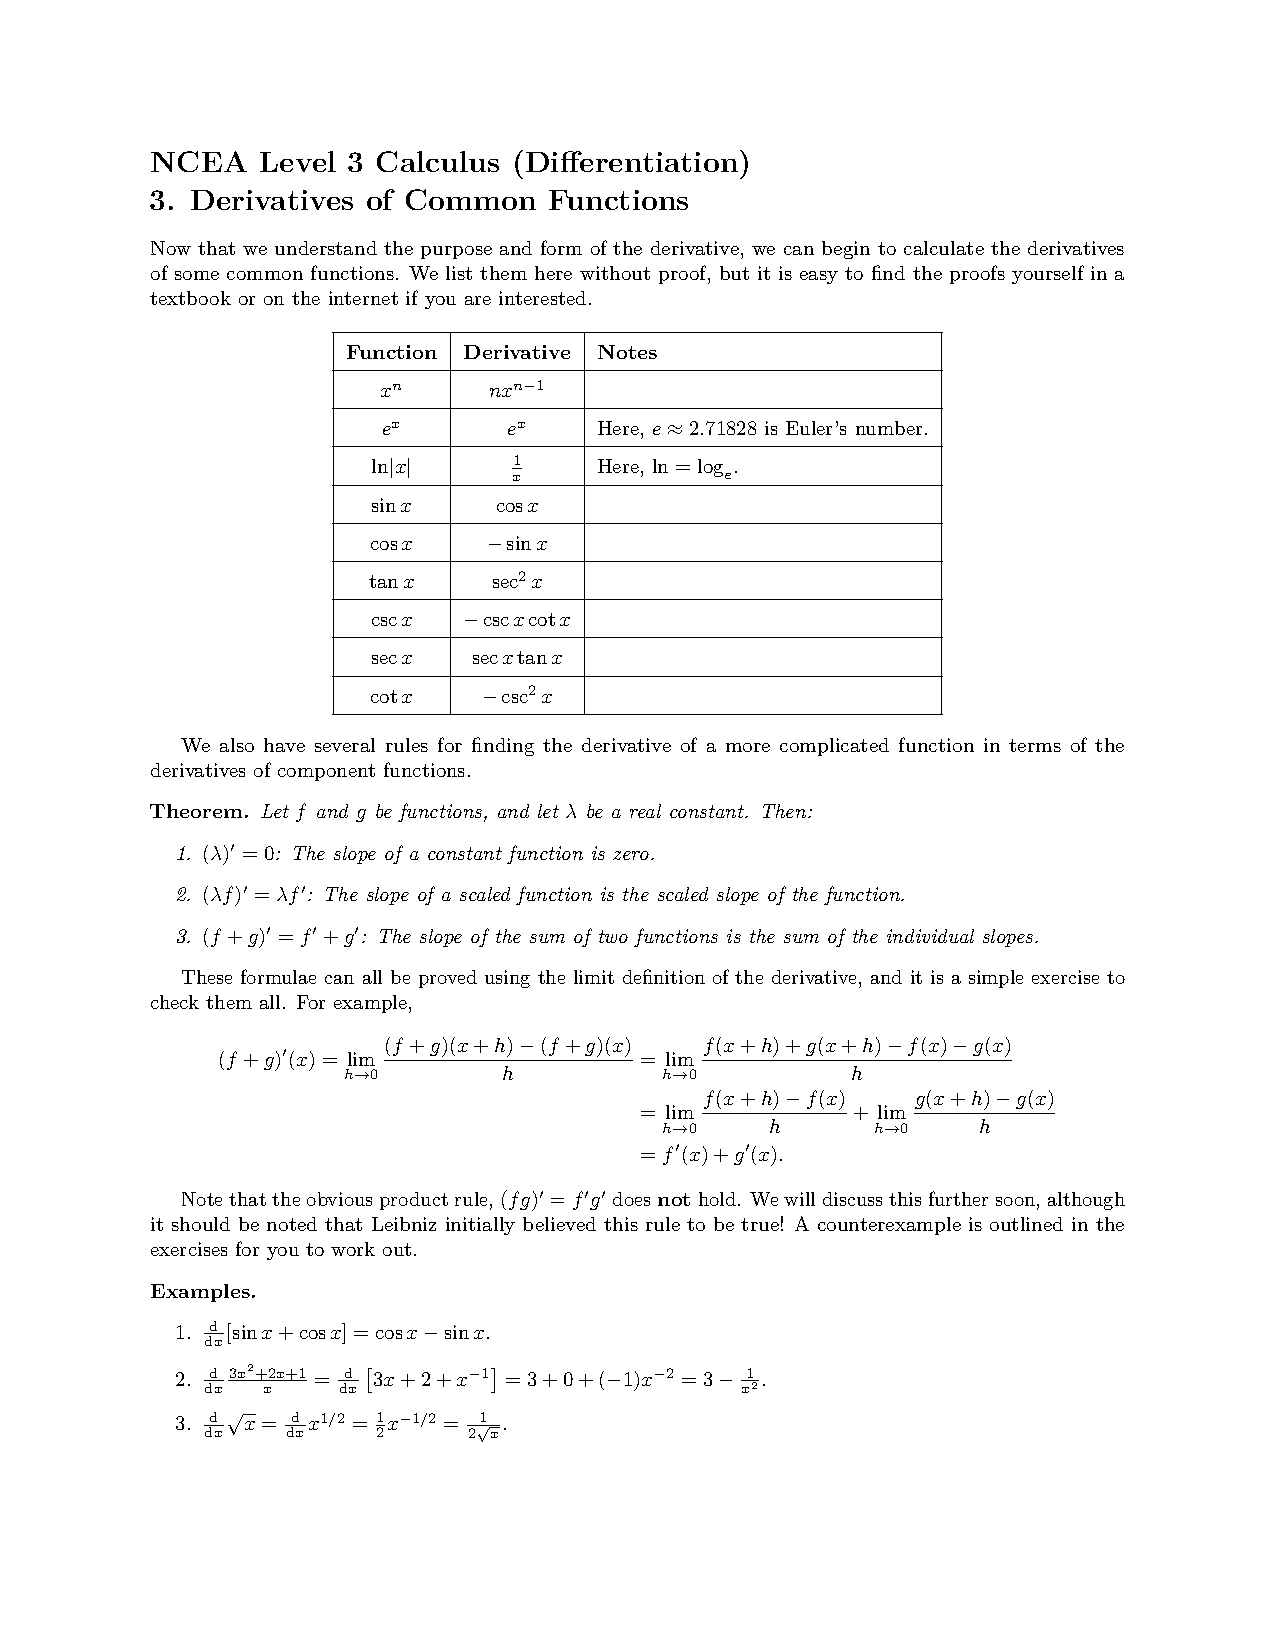
\includepdf[pages={-},pagecommand={}]{03-functions.pdf}
  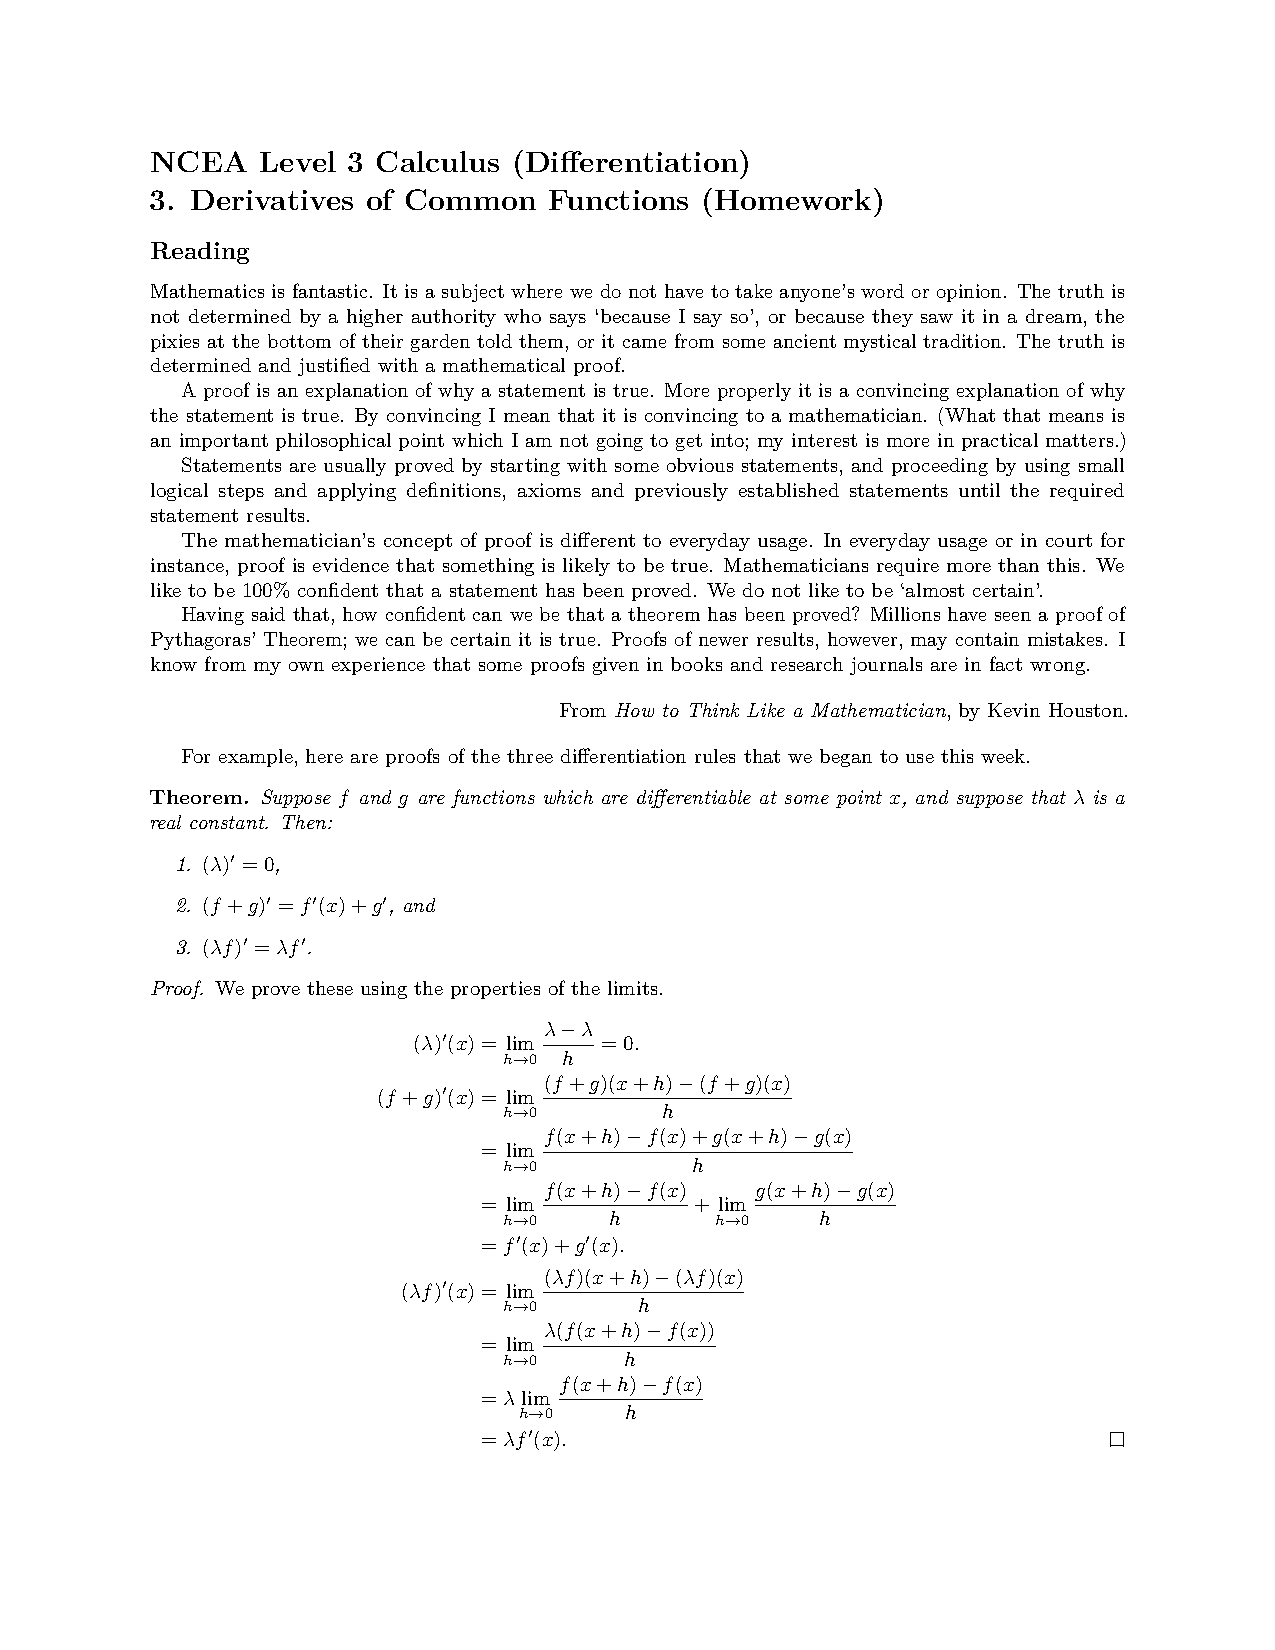
\includepdf[pages={-},pagecommand={}]{03-functions-hw.pdf}
  \phantomsection\addcontentsline{toc}{section}{4. The Chain Rule}
  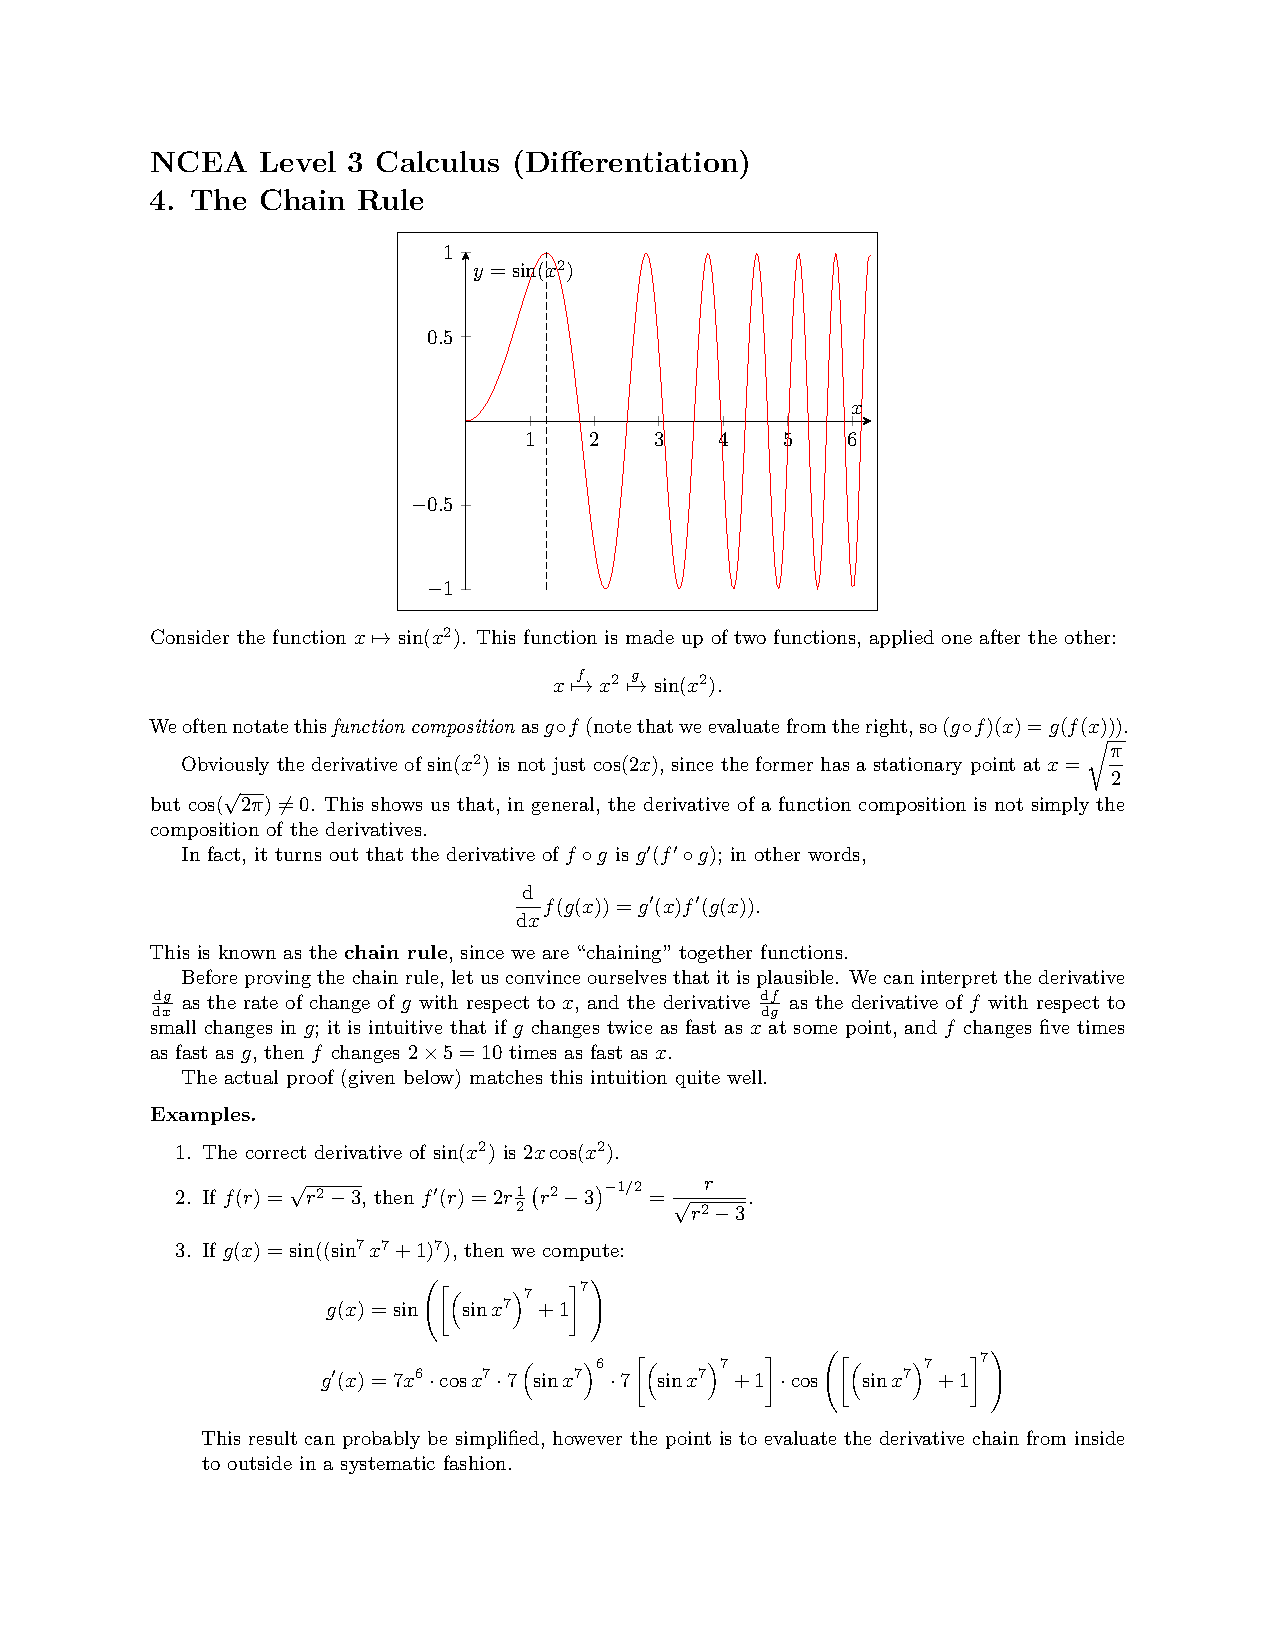
\includepdf[pages={-},pagecommand={}]{04-chainrule.pdf}
  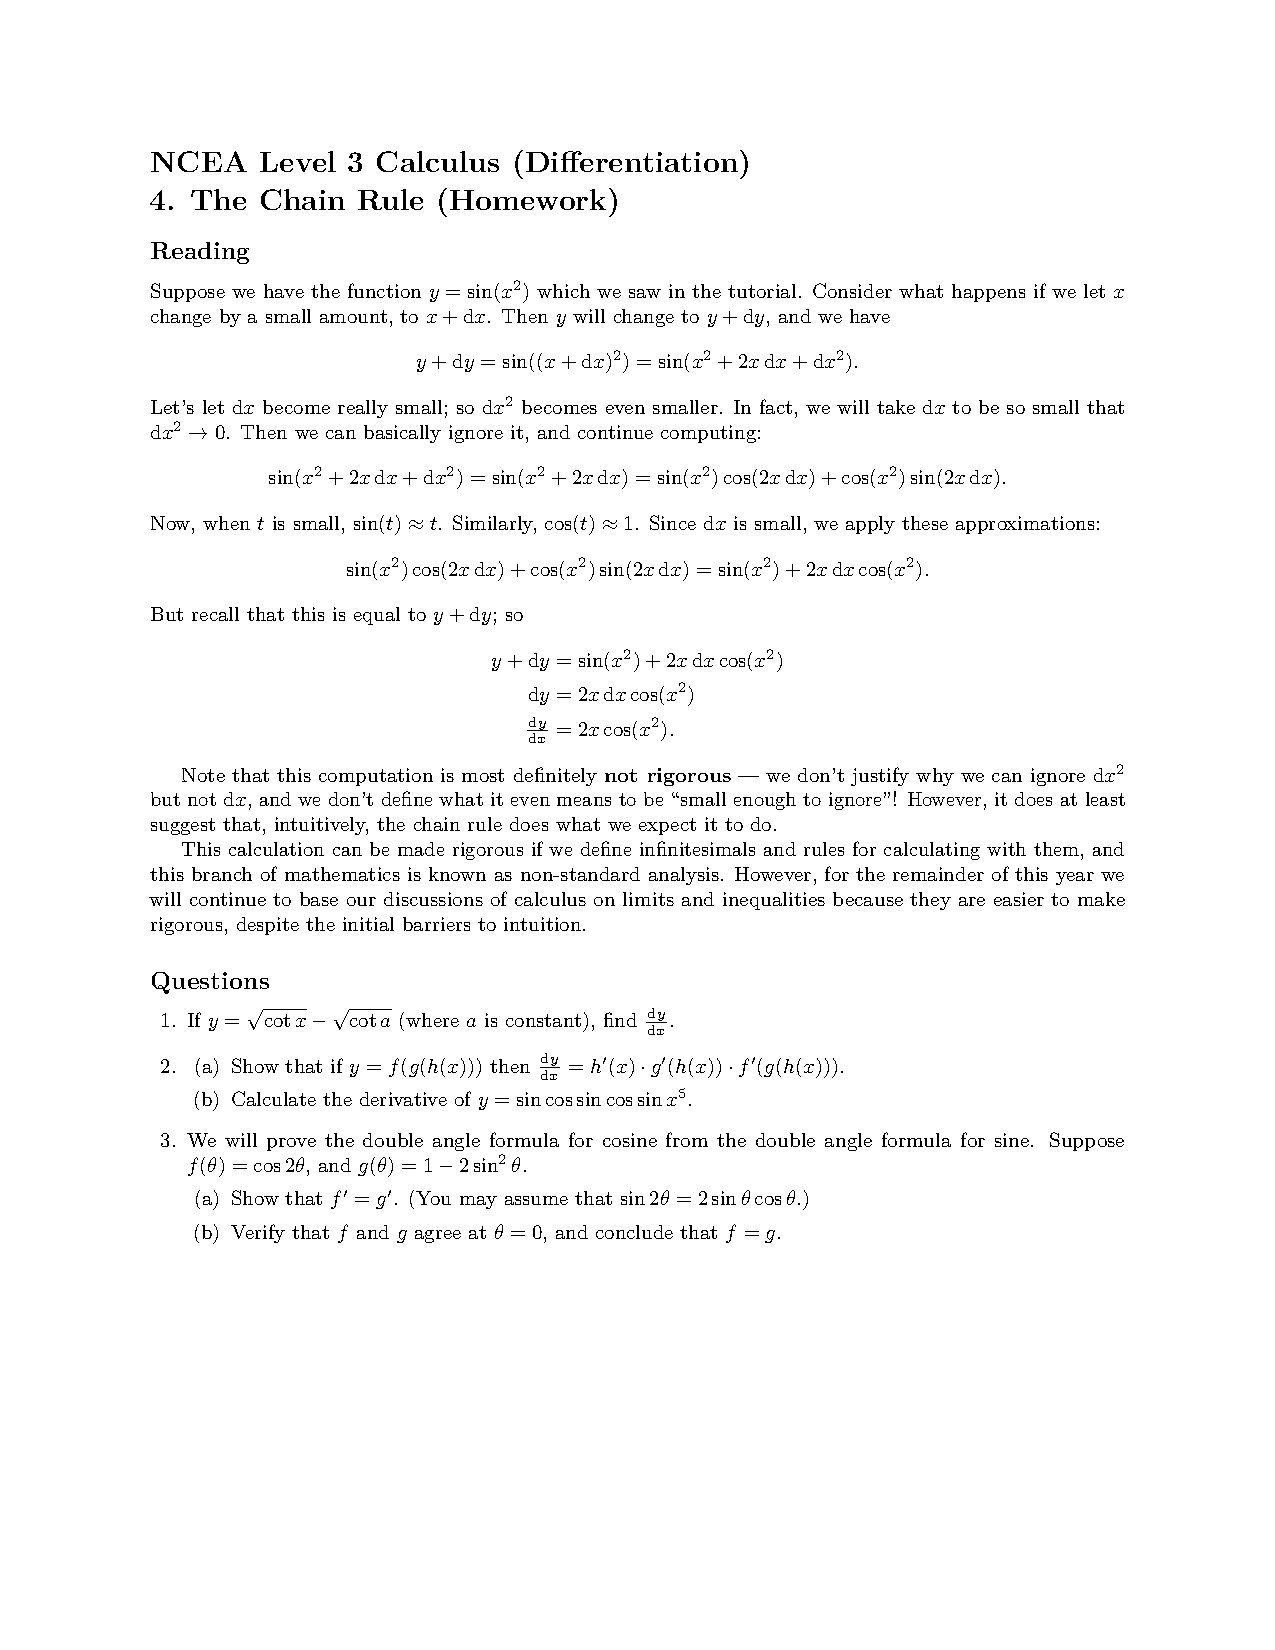
\includepdf[pages={-},pagecommand={}]{04-chainrule-hw.pdf}
  \phantomsection\addcontentsline{toc}{section}{5. The Product and Quotient Rules}
  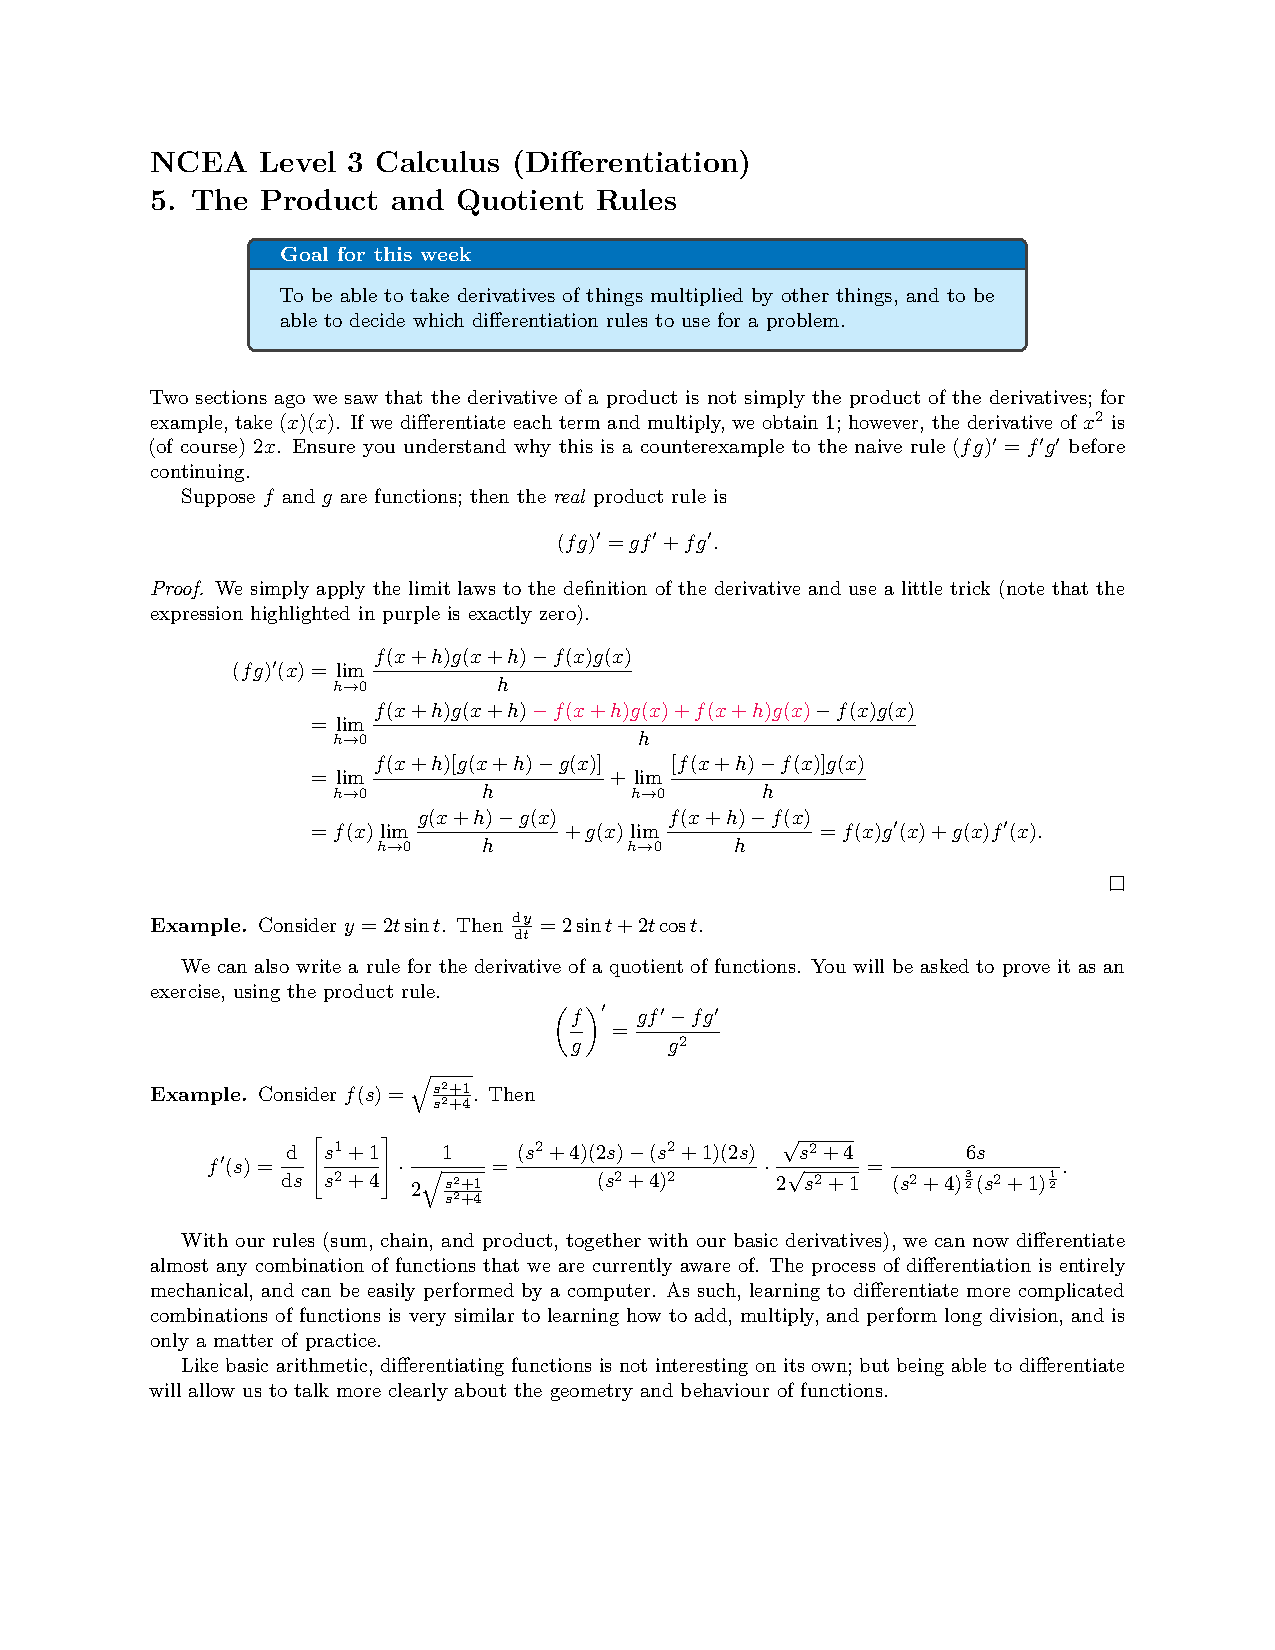
\includepdf[pages={-},pagecommand={}]{05-prodandquo.pdf}
  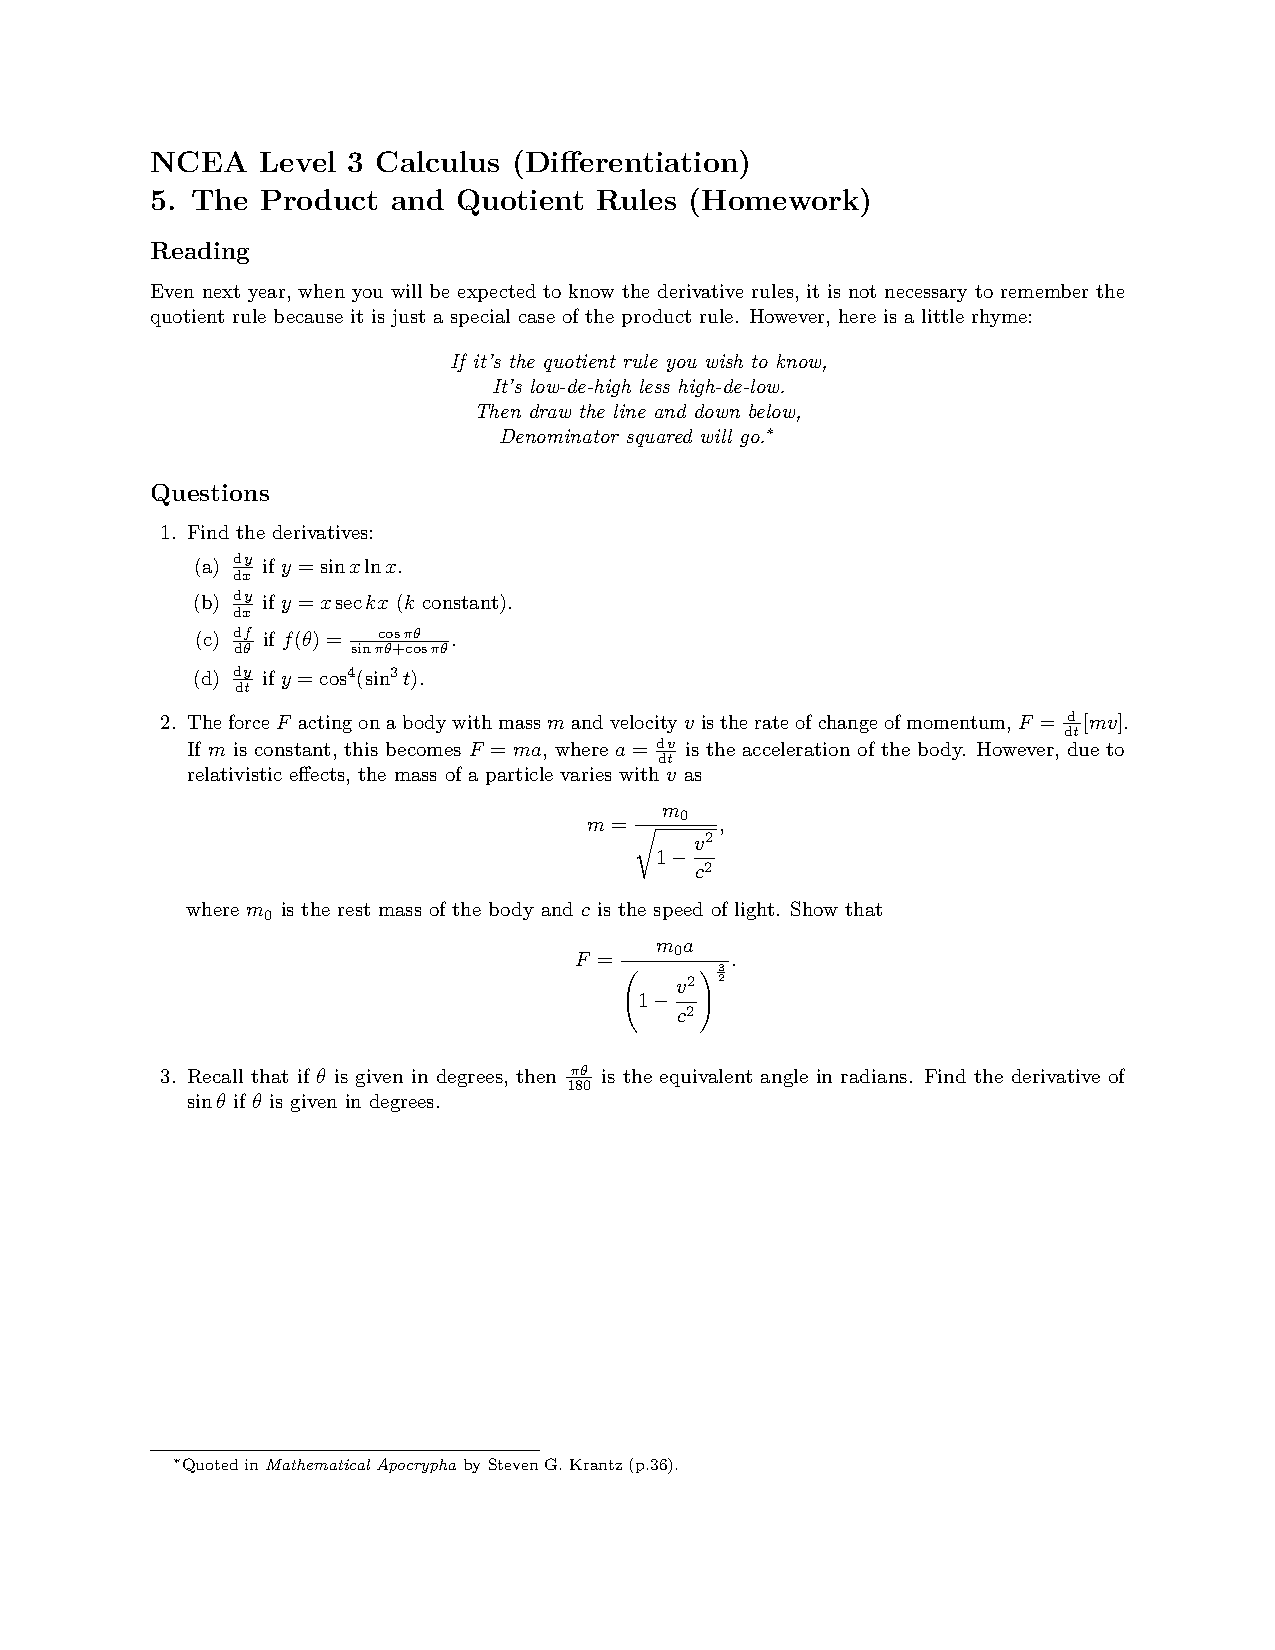
\includepdf[pages={-},pagecommand={}]{05-prodandquo-hw.pdf}
  \phantomsection\addcontentsline{toc}{section}{6. Tangent and Normal Lines}
  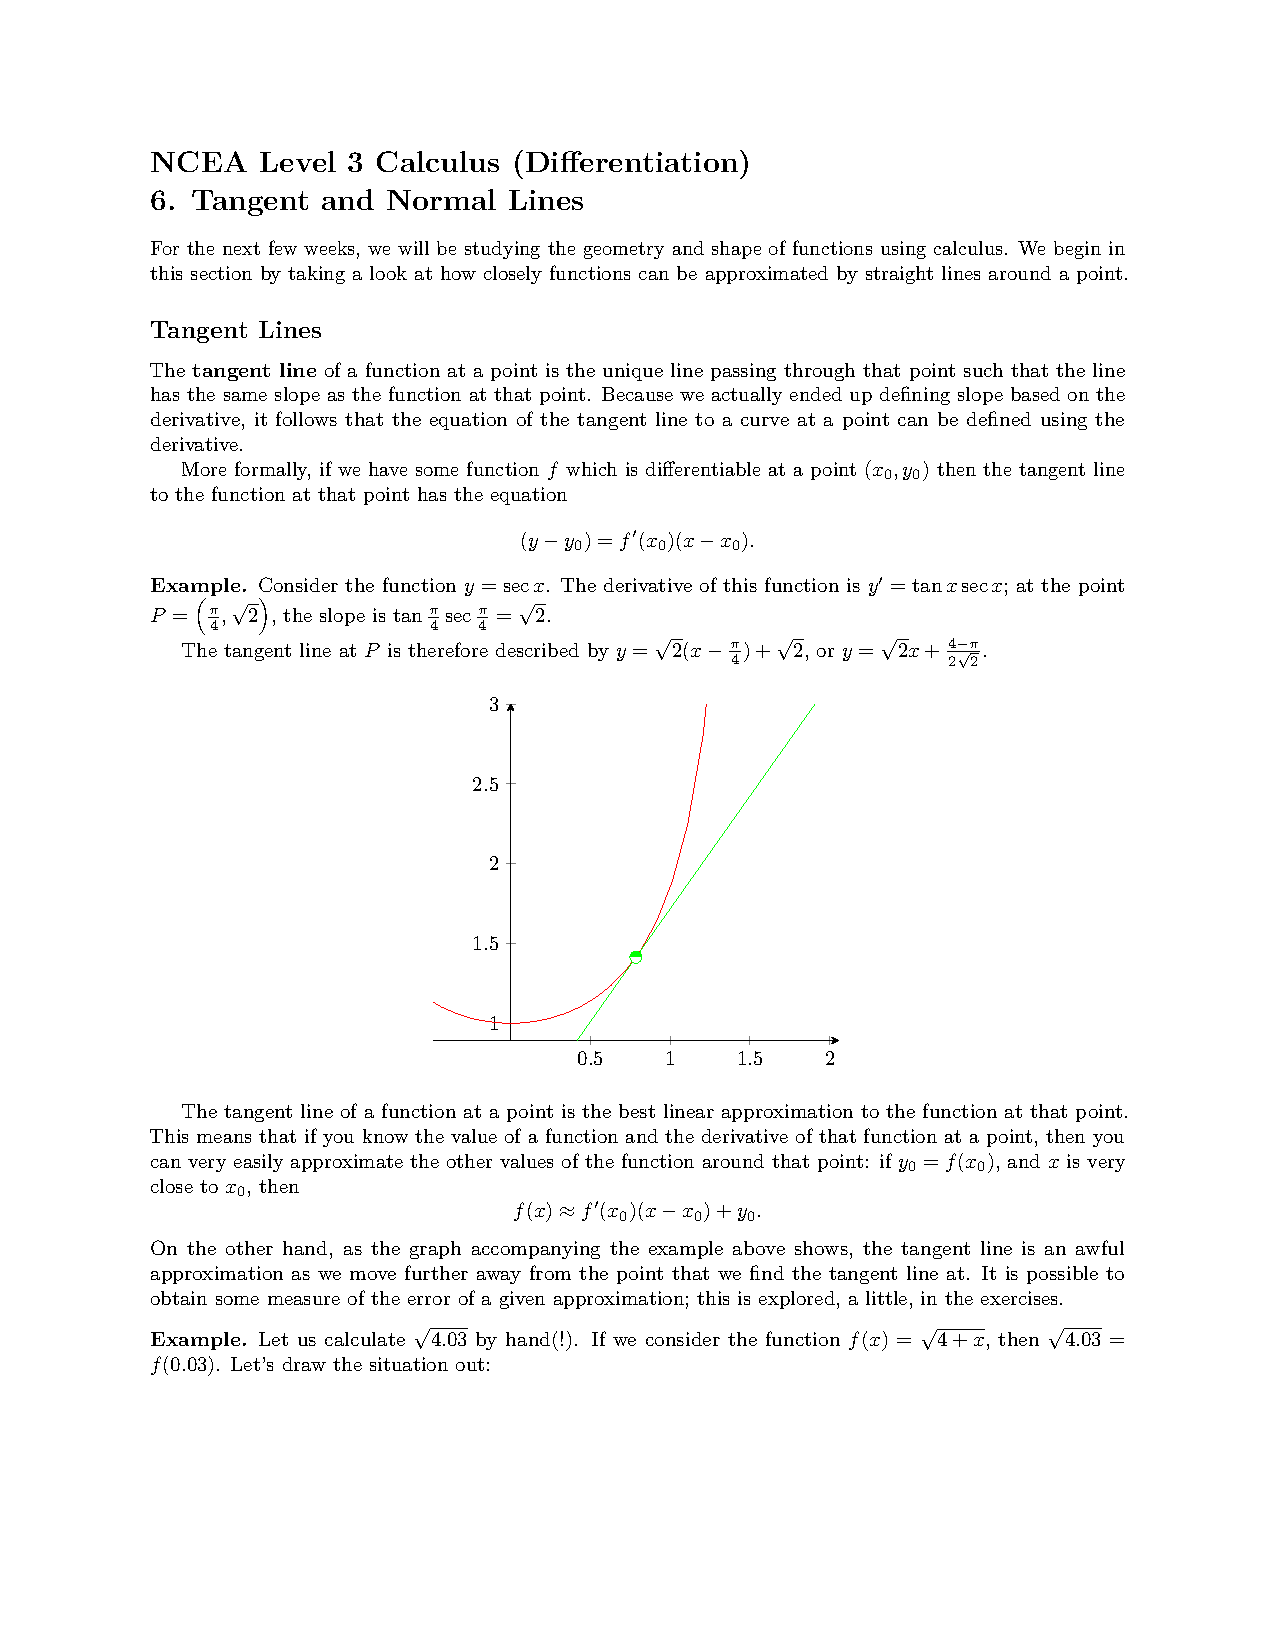
\includepdf[pages={-},pagecommand={}]{06-tanolines.pdf}
  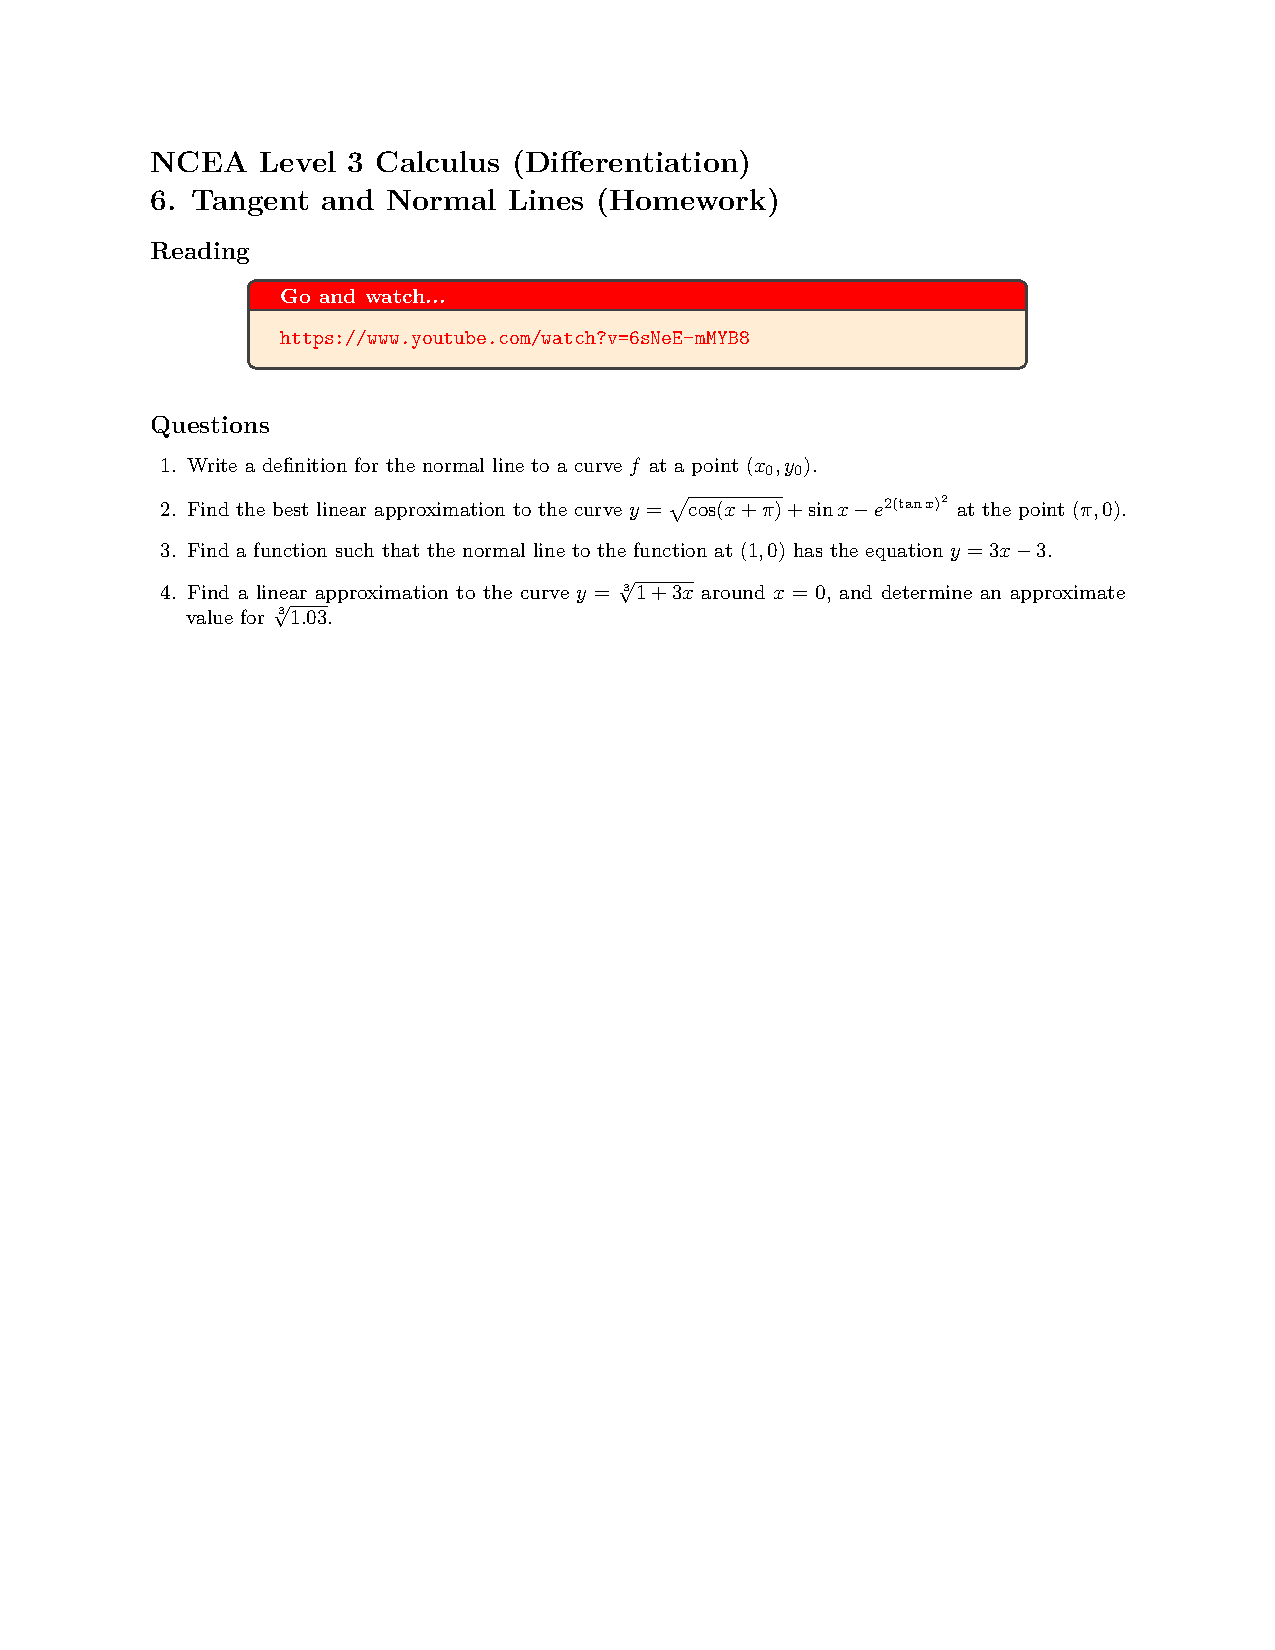
\includepdf[pages={-},pagecommand={}]{06-tanolines-hw.pdf}
  \phantomsection\addcontentsline{toc}{section}{7. The Geometry of Functions}
  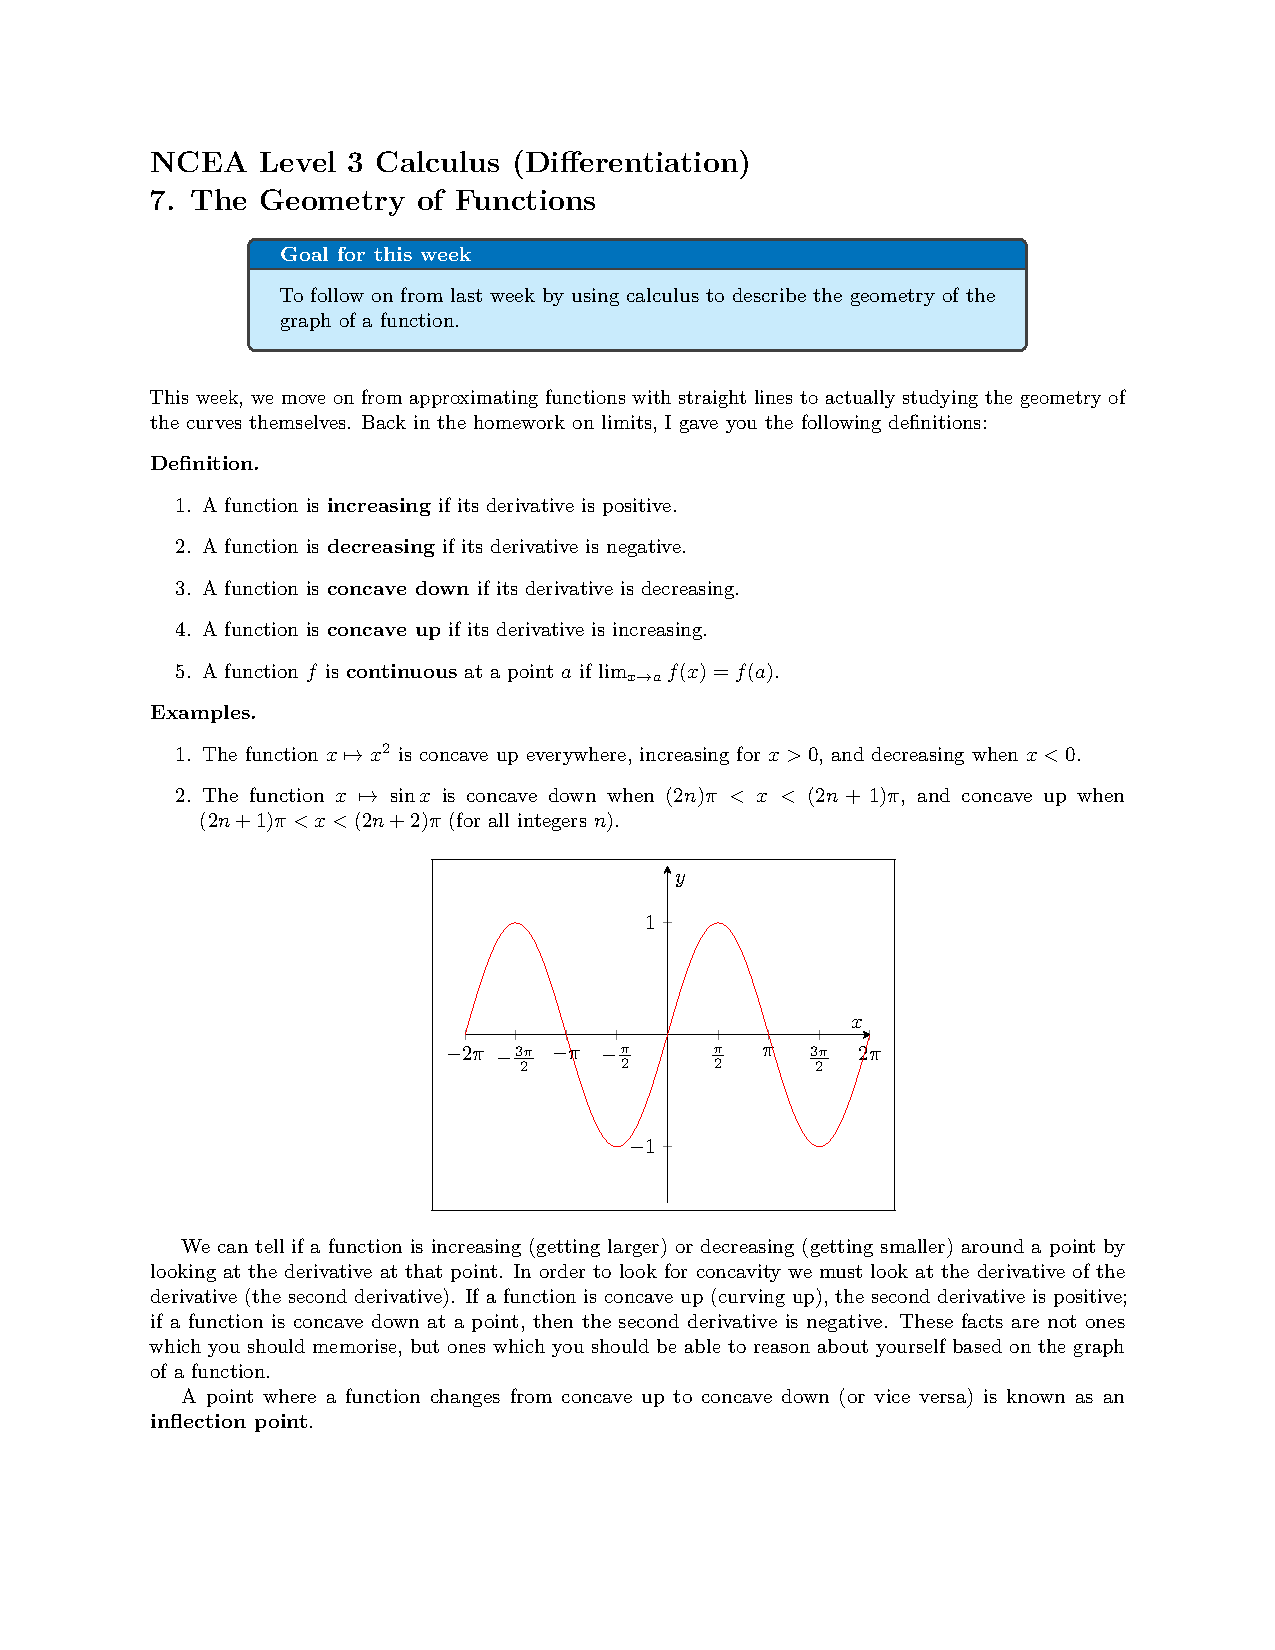
\includepdf[pages={-},pagecommand={}]{07-geometry2.pdf}
  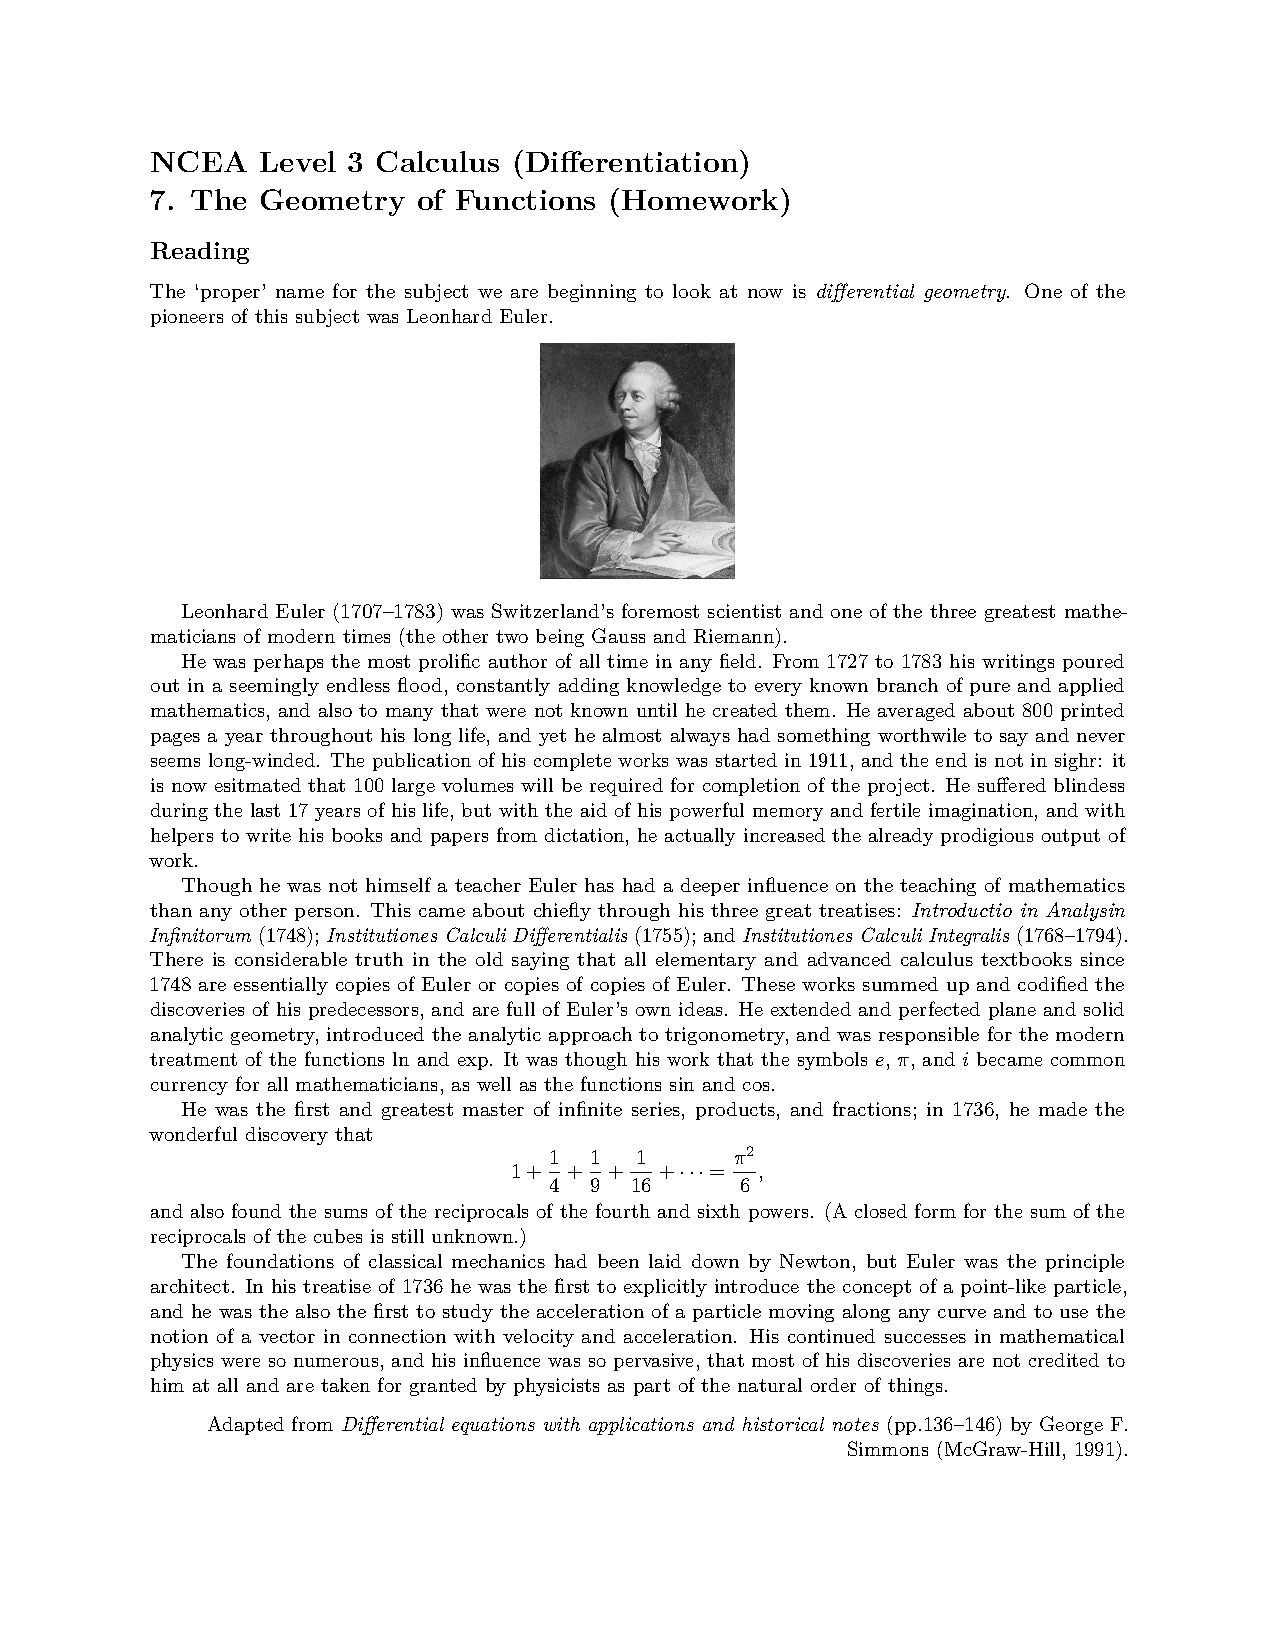
\includepdf[pages={-},pagecommand={}]{07-geometry2-hw.pdf}
  \phantomsection\addcontentsline{toc}{section}{Differentiation Assignment}
  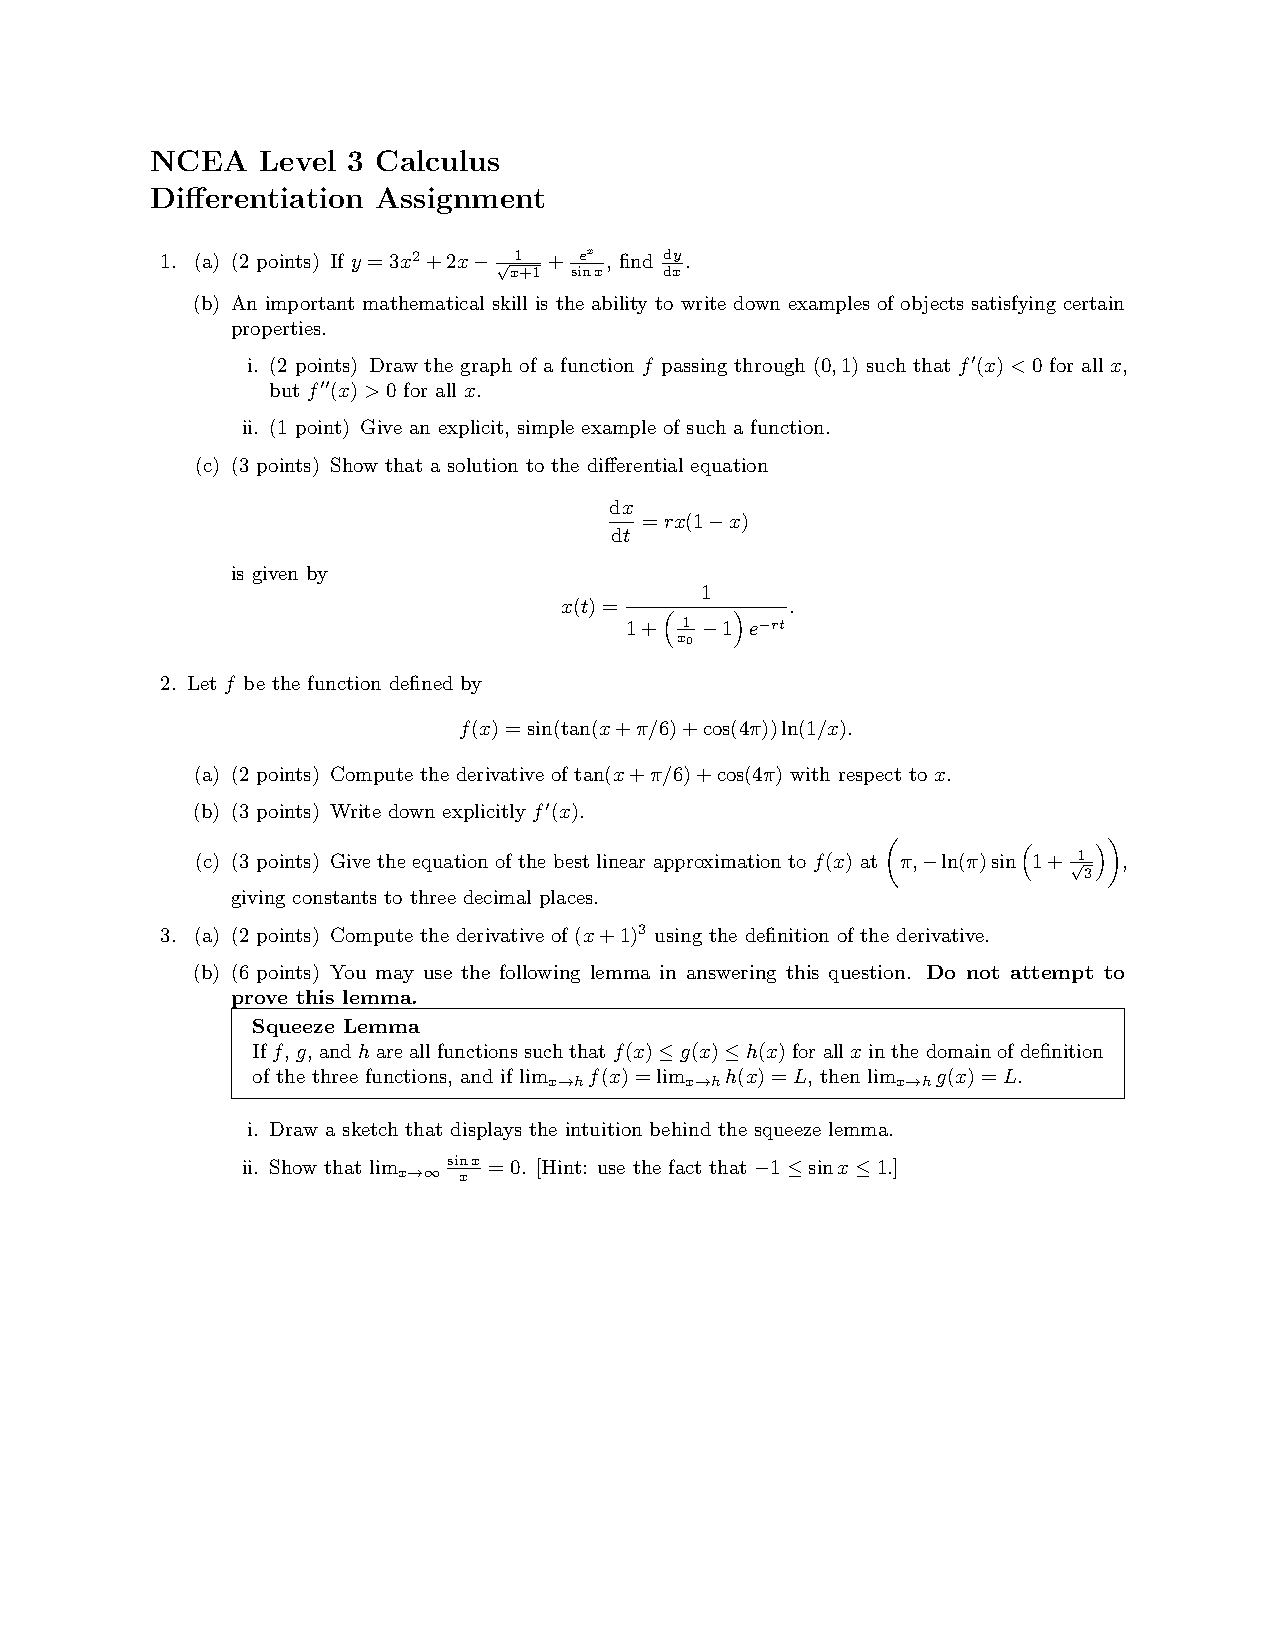
\includepdf[pages={-},pagecommand={}]{asst-differentiation.pdf}
  \phantomsection\addcontentsline{toc}{section}{8. Optimisation}
  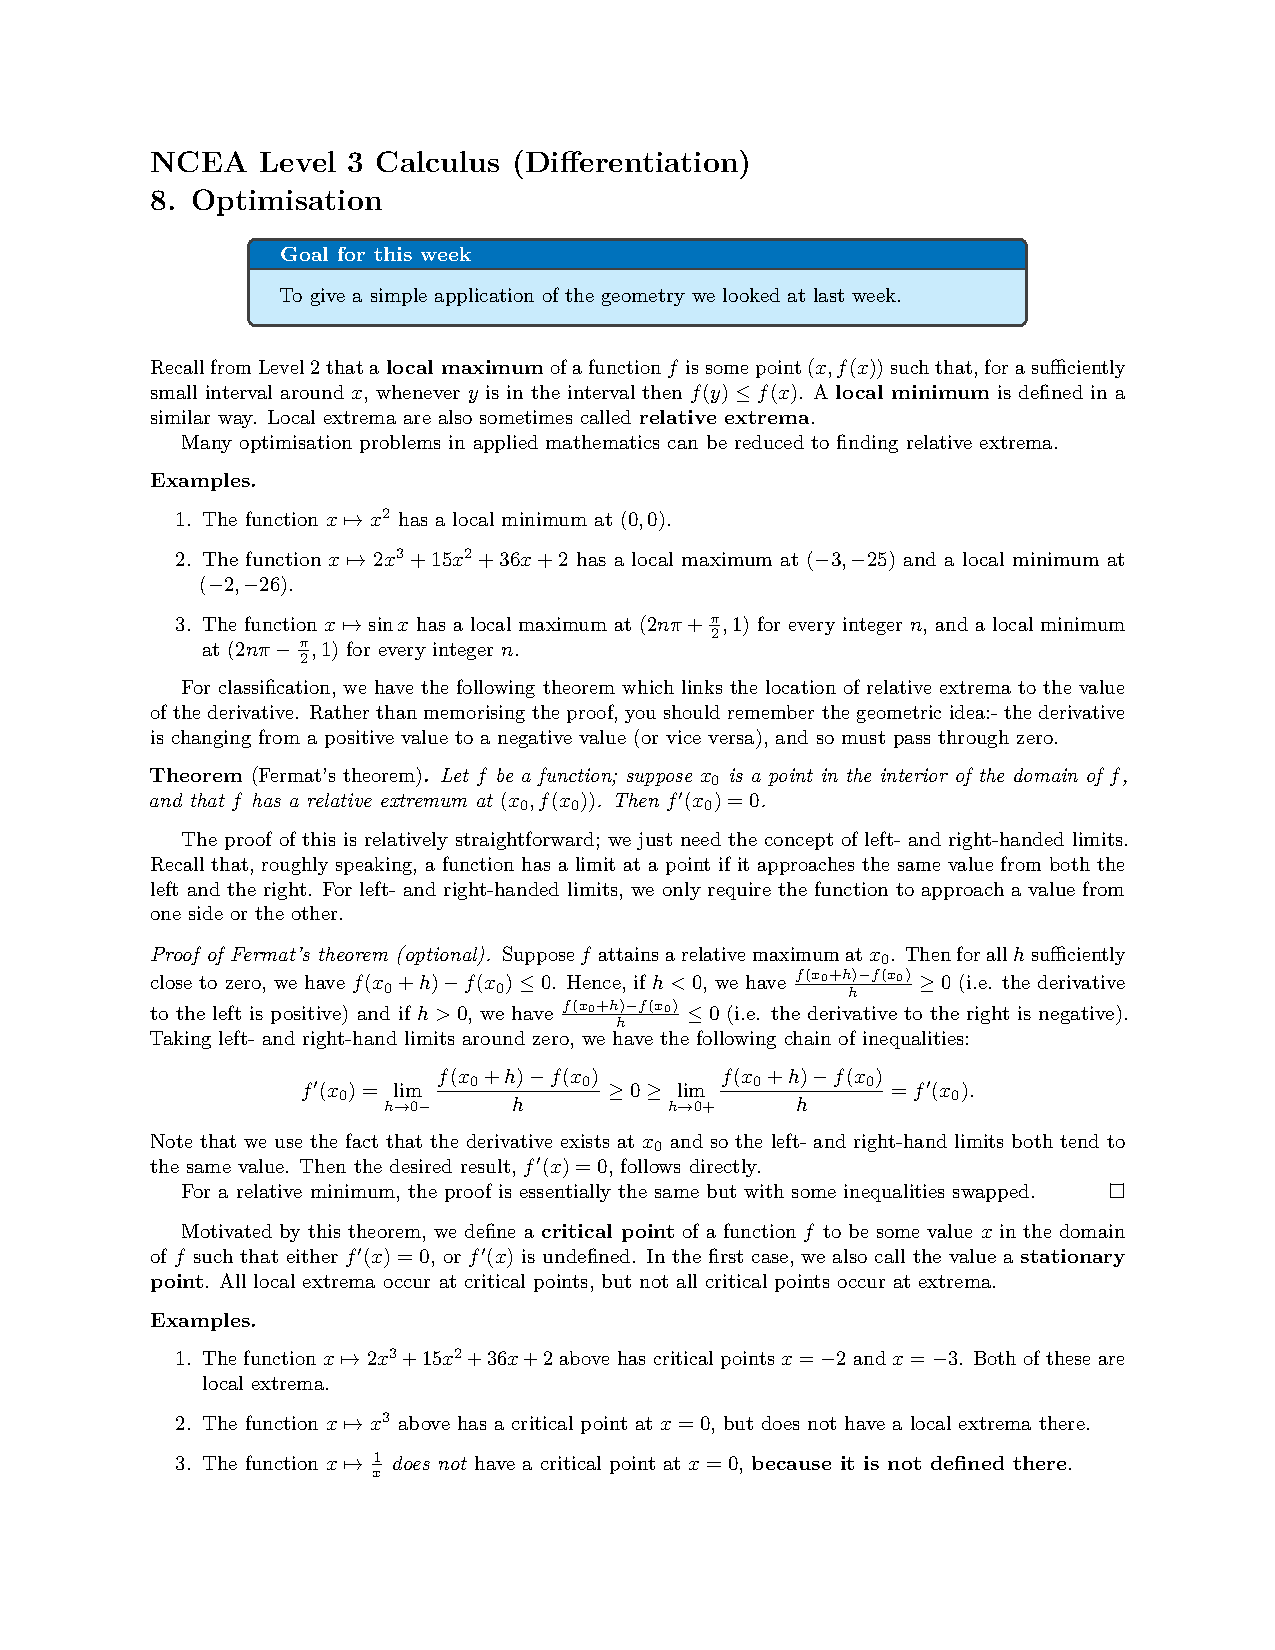
\includepdf[pages={-},pagecommand={}]{08-maxamin.pdf}
  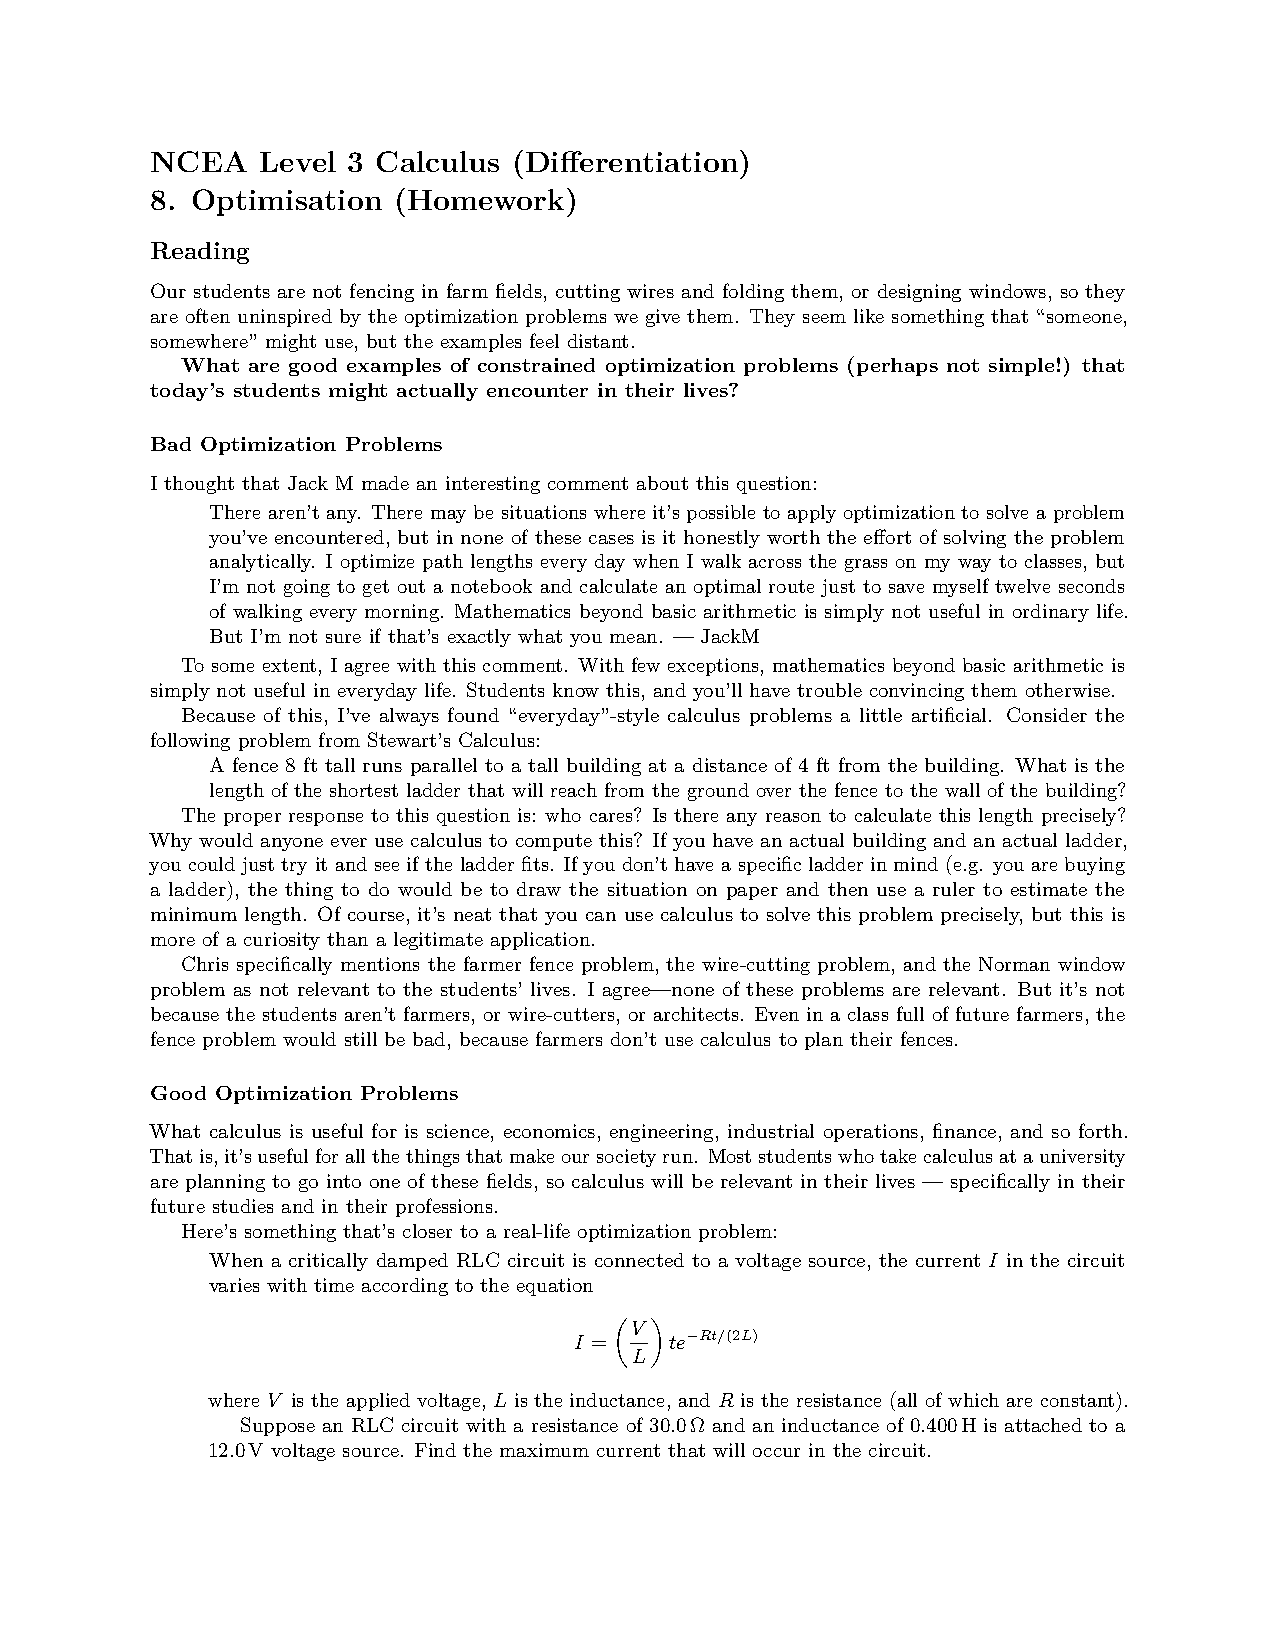
\includepdf[pages={-},pagecommand={}]{08-maxamin-hw.pdf}
  \phantomsection\addcontentsline{toc}{section}{9. Implicit Differentiation}
  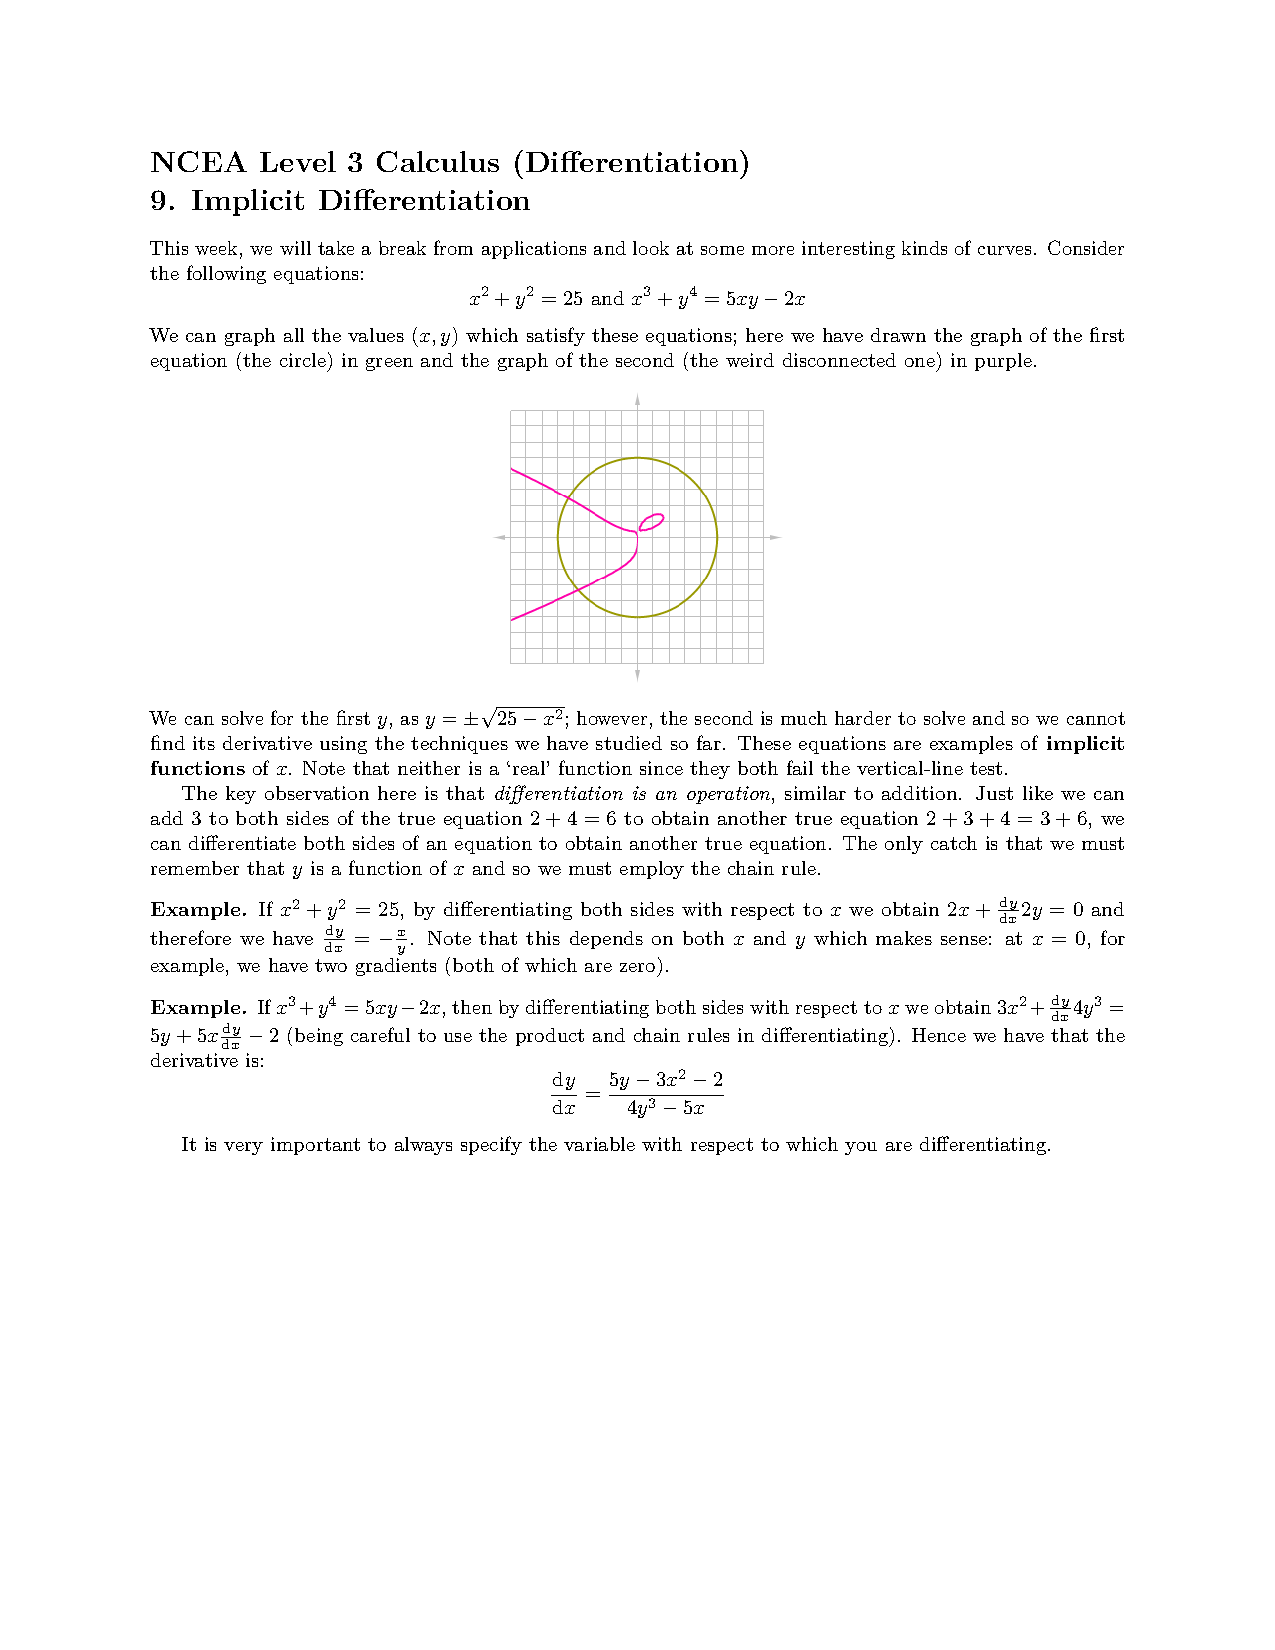
\includepdf[pages={-},pagecommand={}]{09-implicit.pdf}
  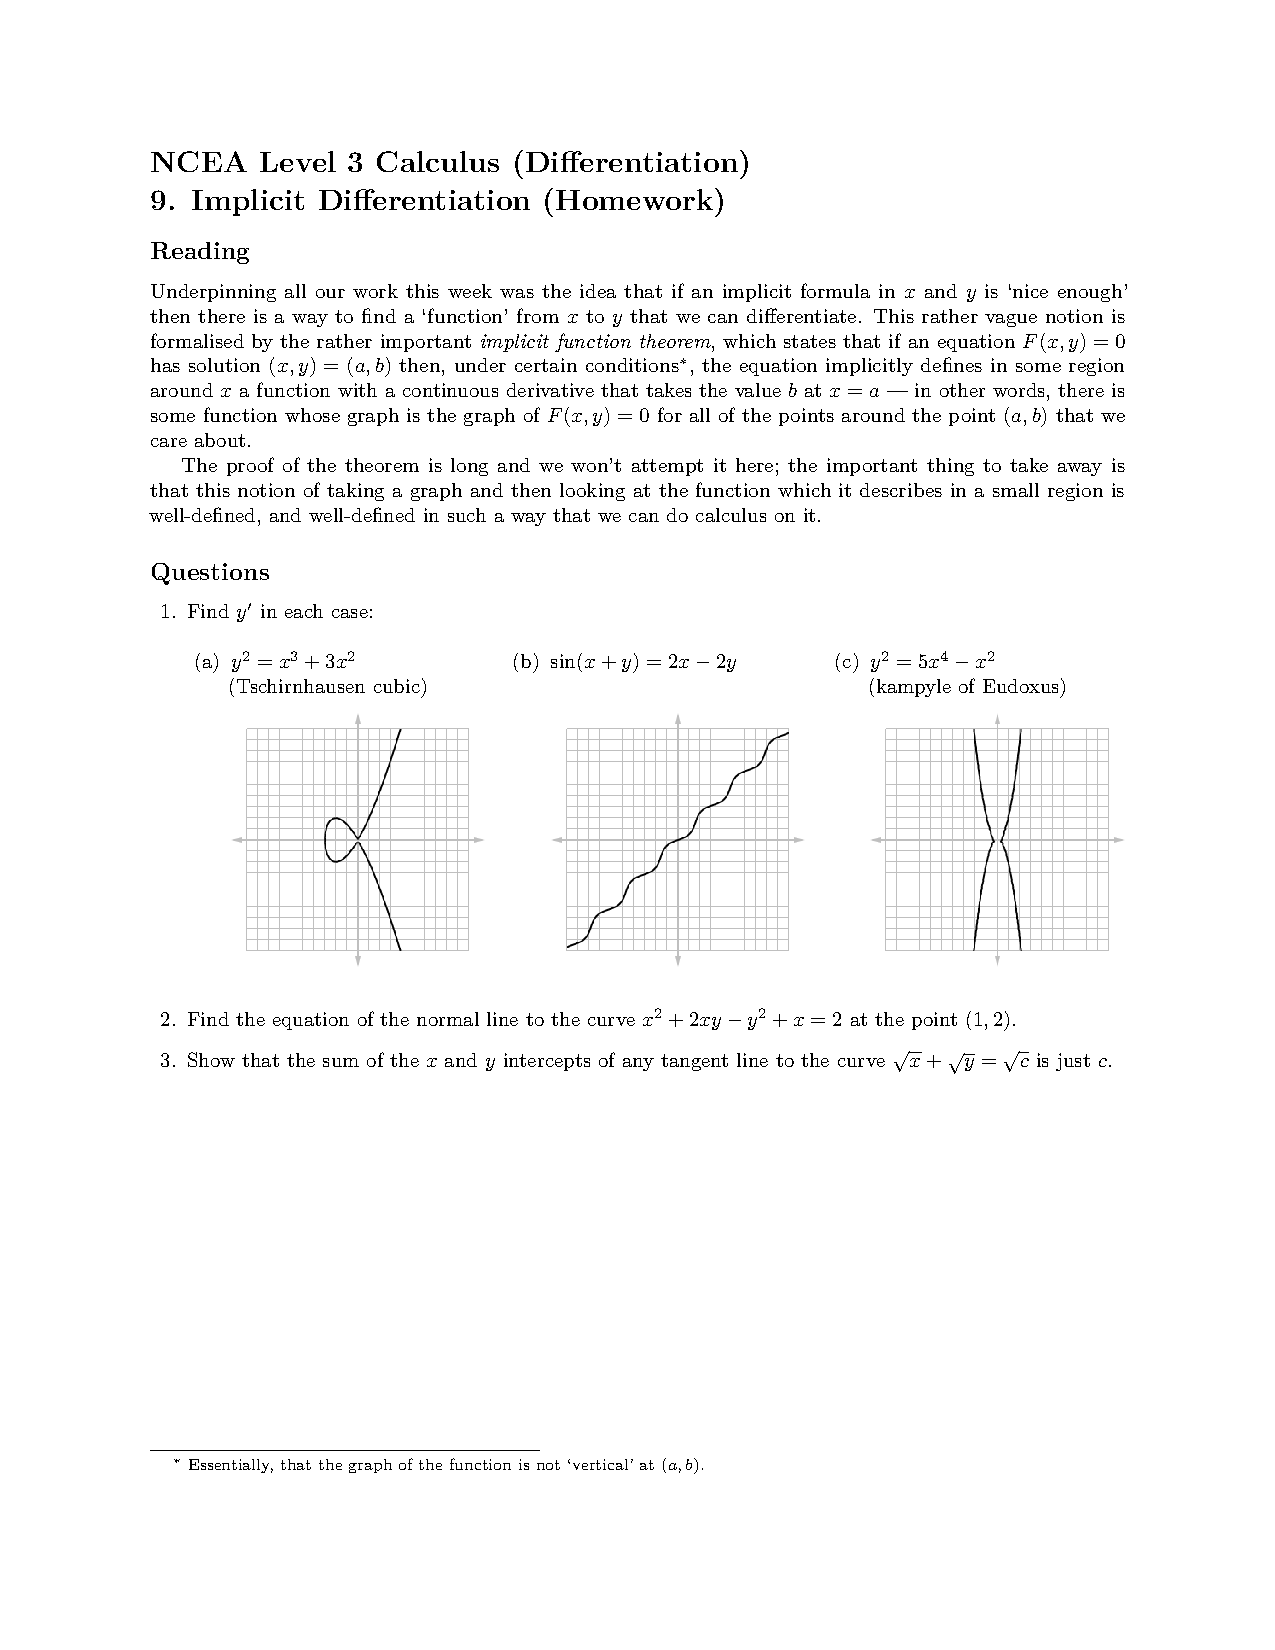
\includepdf[pages={-},pagecommand={}]{09-implicit-hw.pdf}
  \phantomsection\addcontentsline{toc}{section}{10. Inverse Functions}
  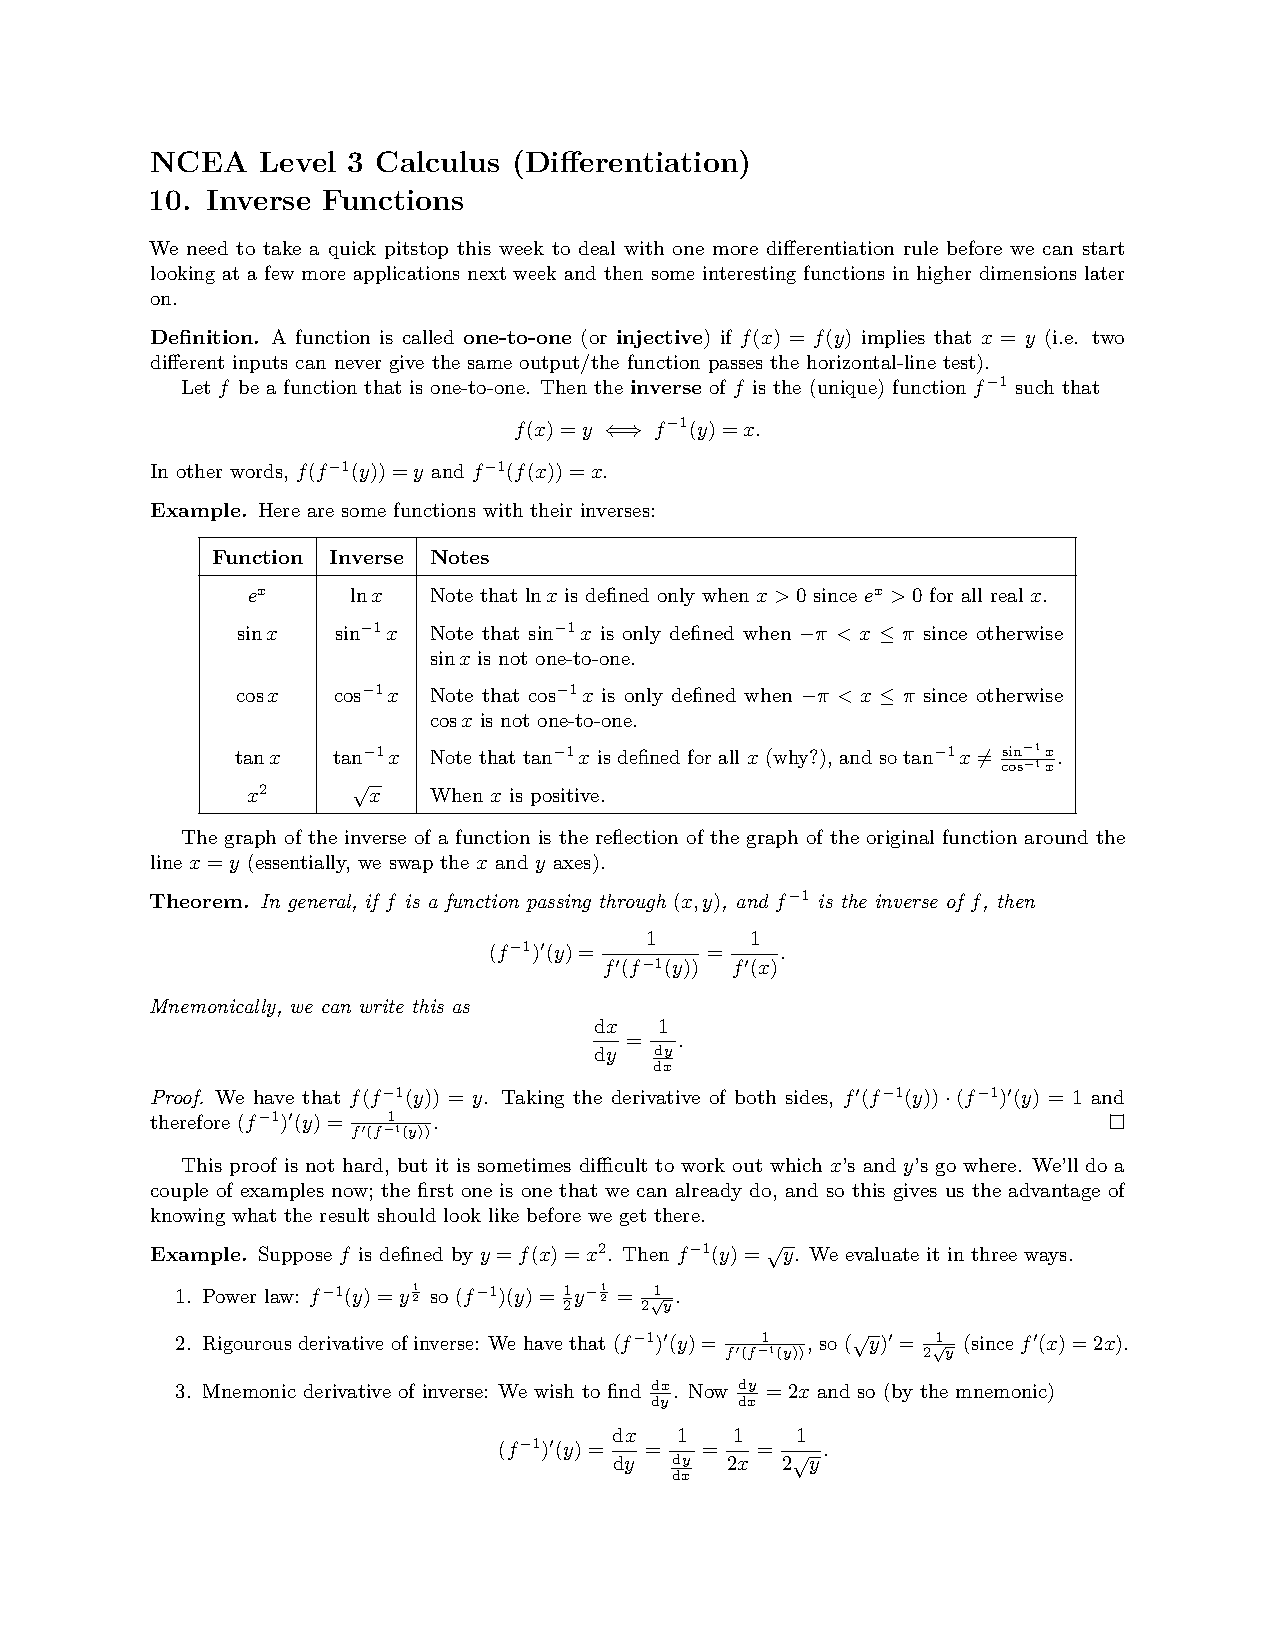
\includepdf[pages={-},pagecommand={}]{10-inverses.pdf}
  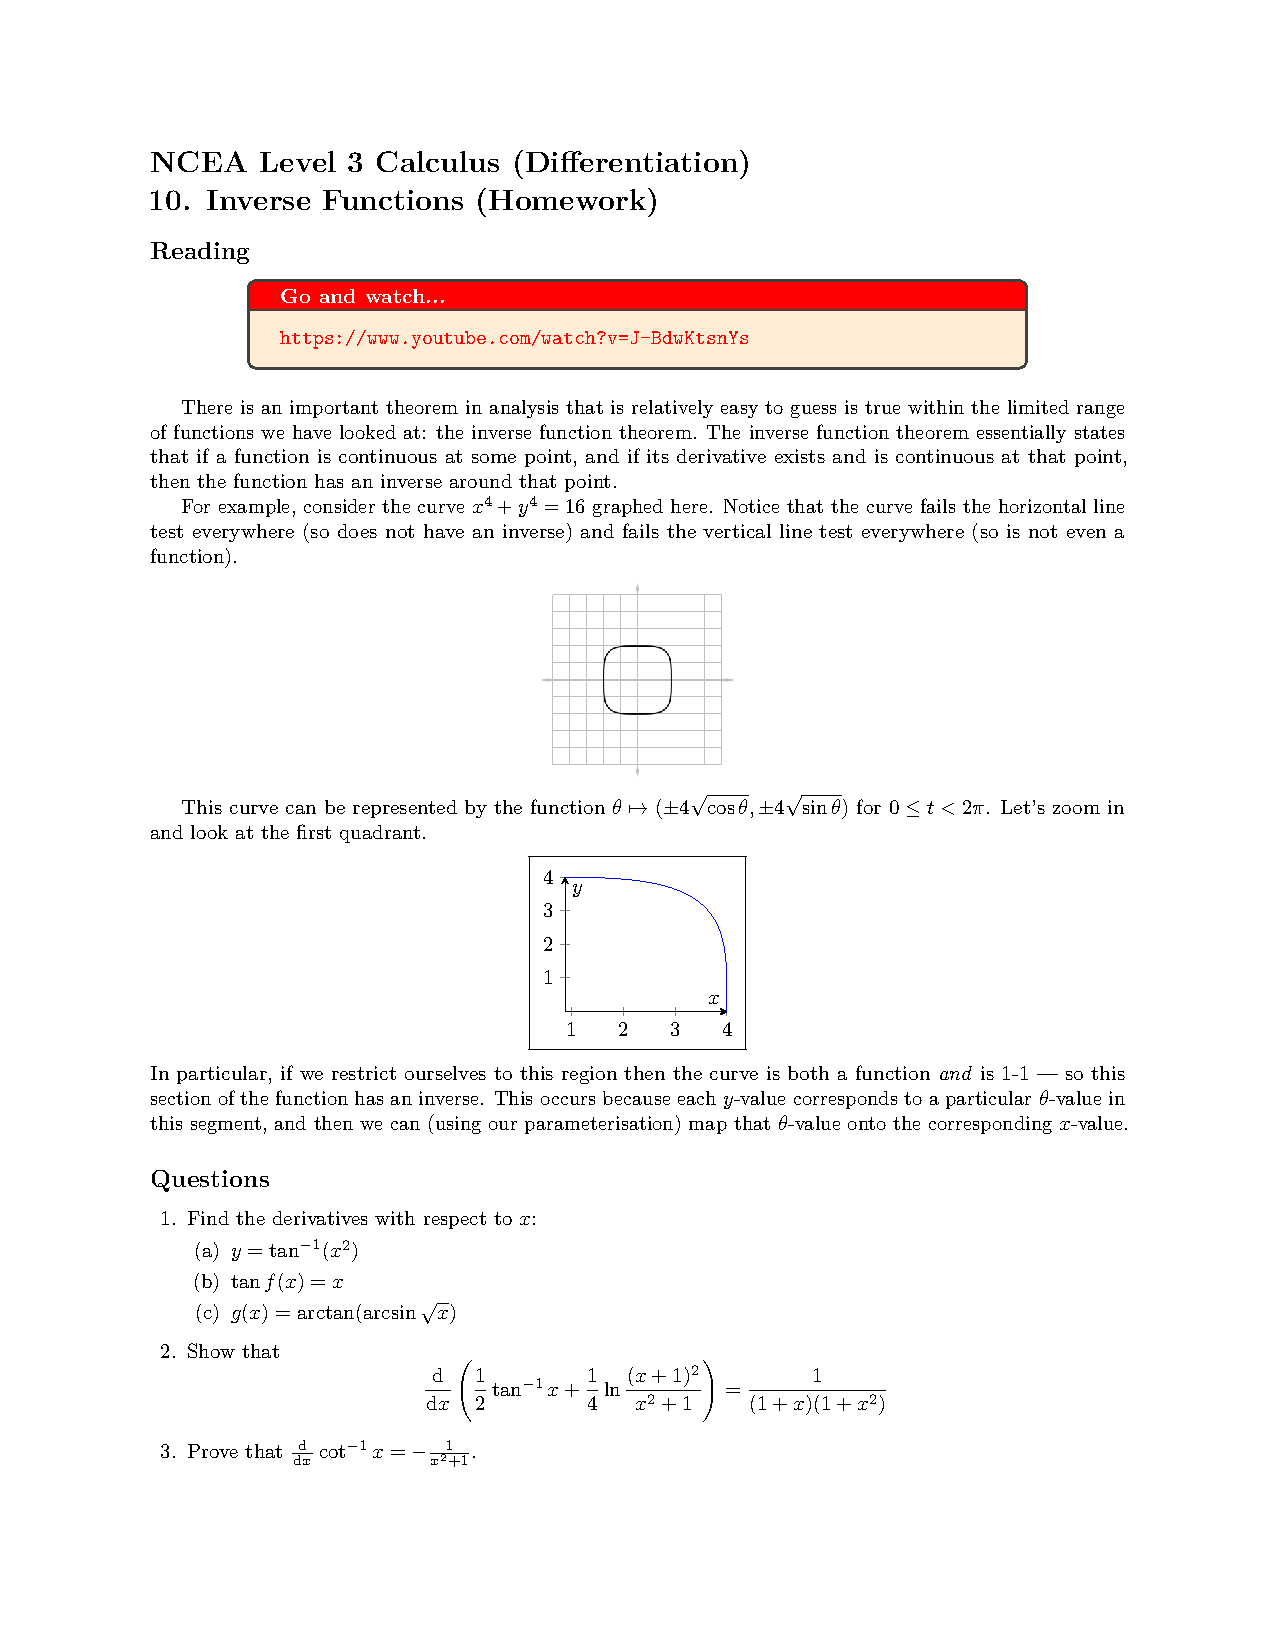
\includepdf[pages={-},pagecommand={}]{10-inverses-hw.pdf}
  \phantomsection\addcontentsline{toc}{section}{11. Related Rates of Change}
  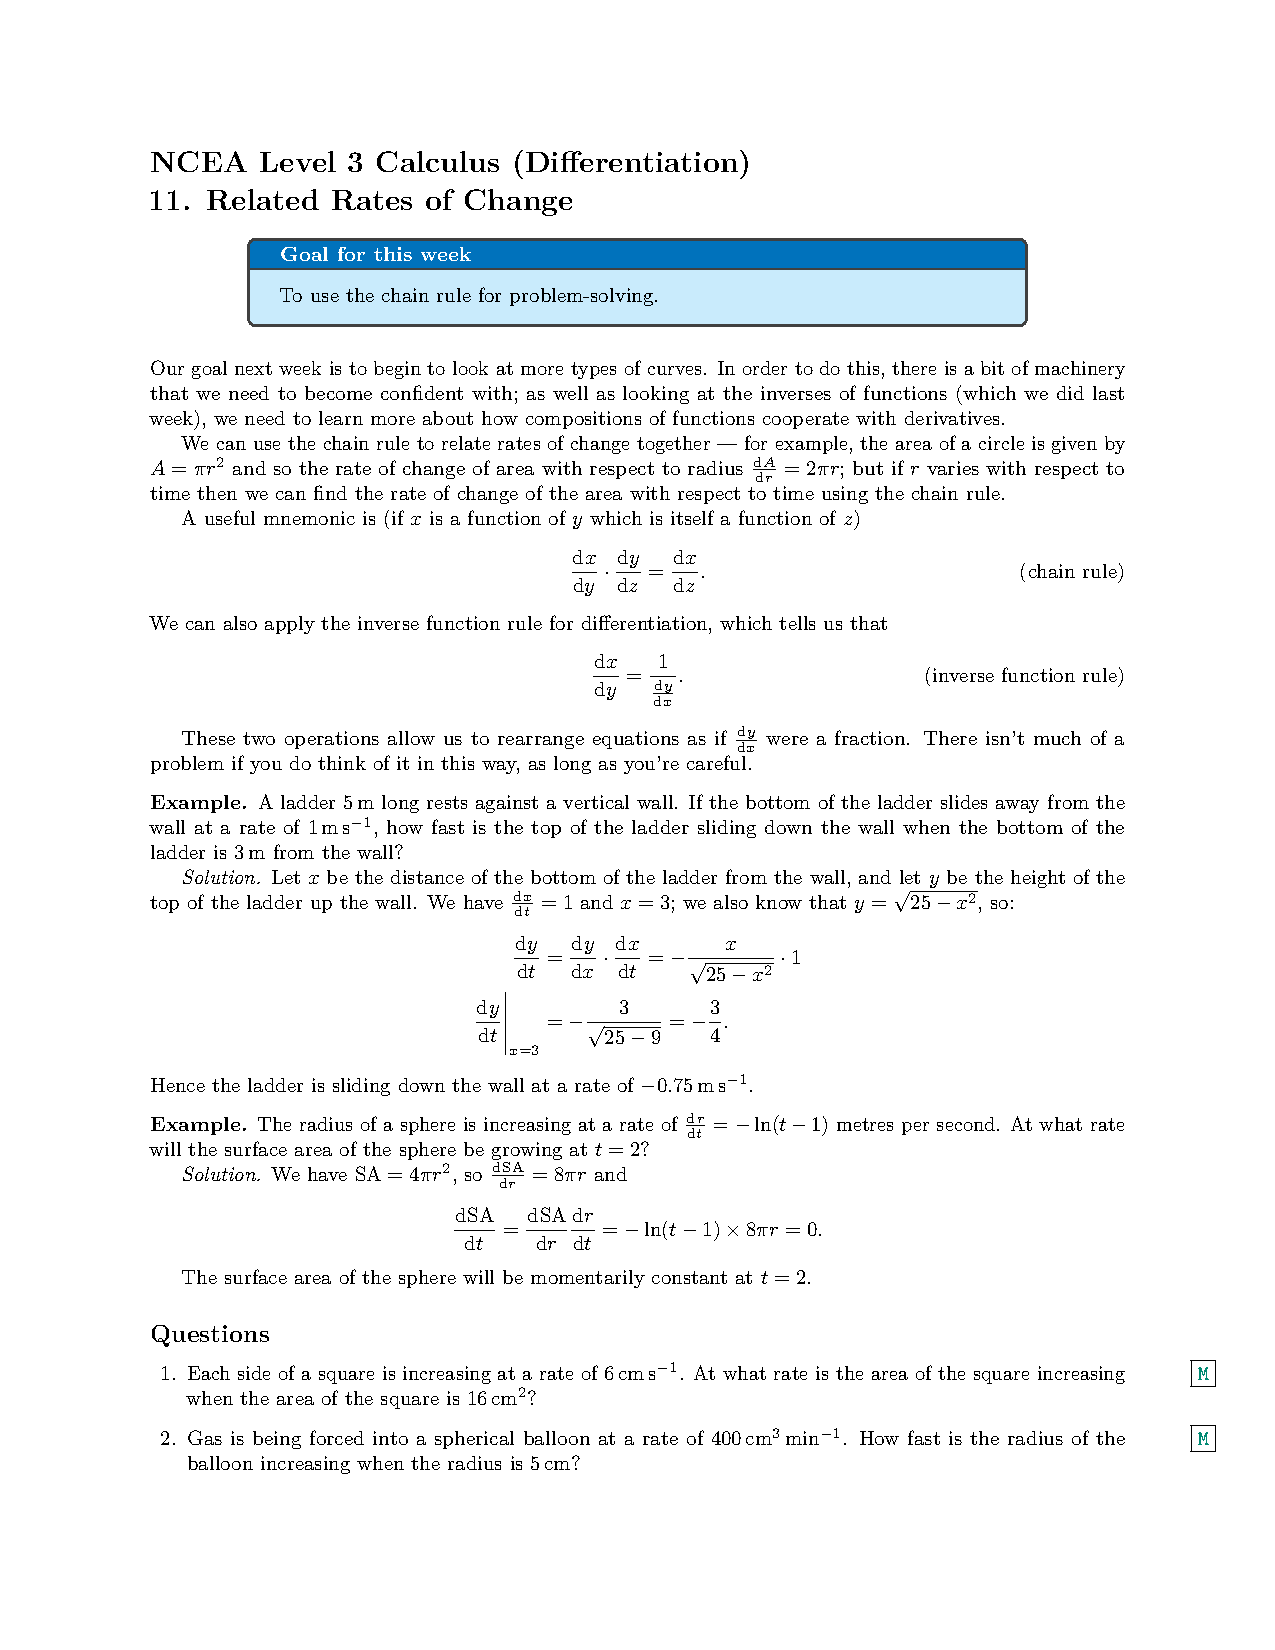
\includepdf[pages={-},pagecommand={}]{11-chainrule2.pdf}
  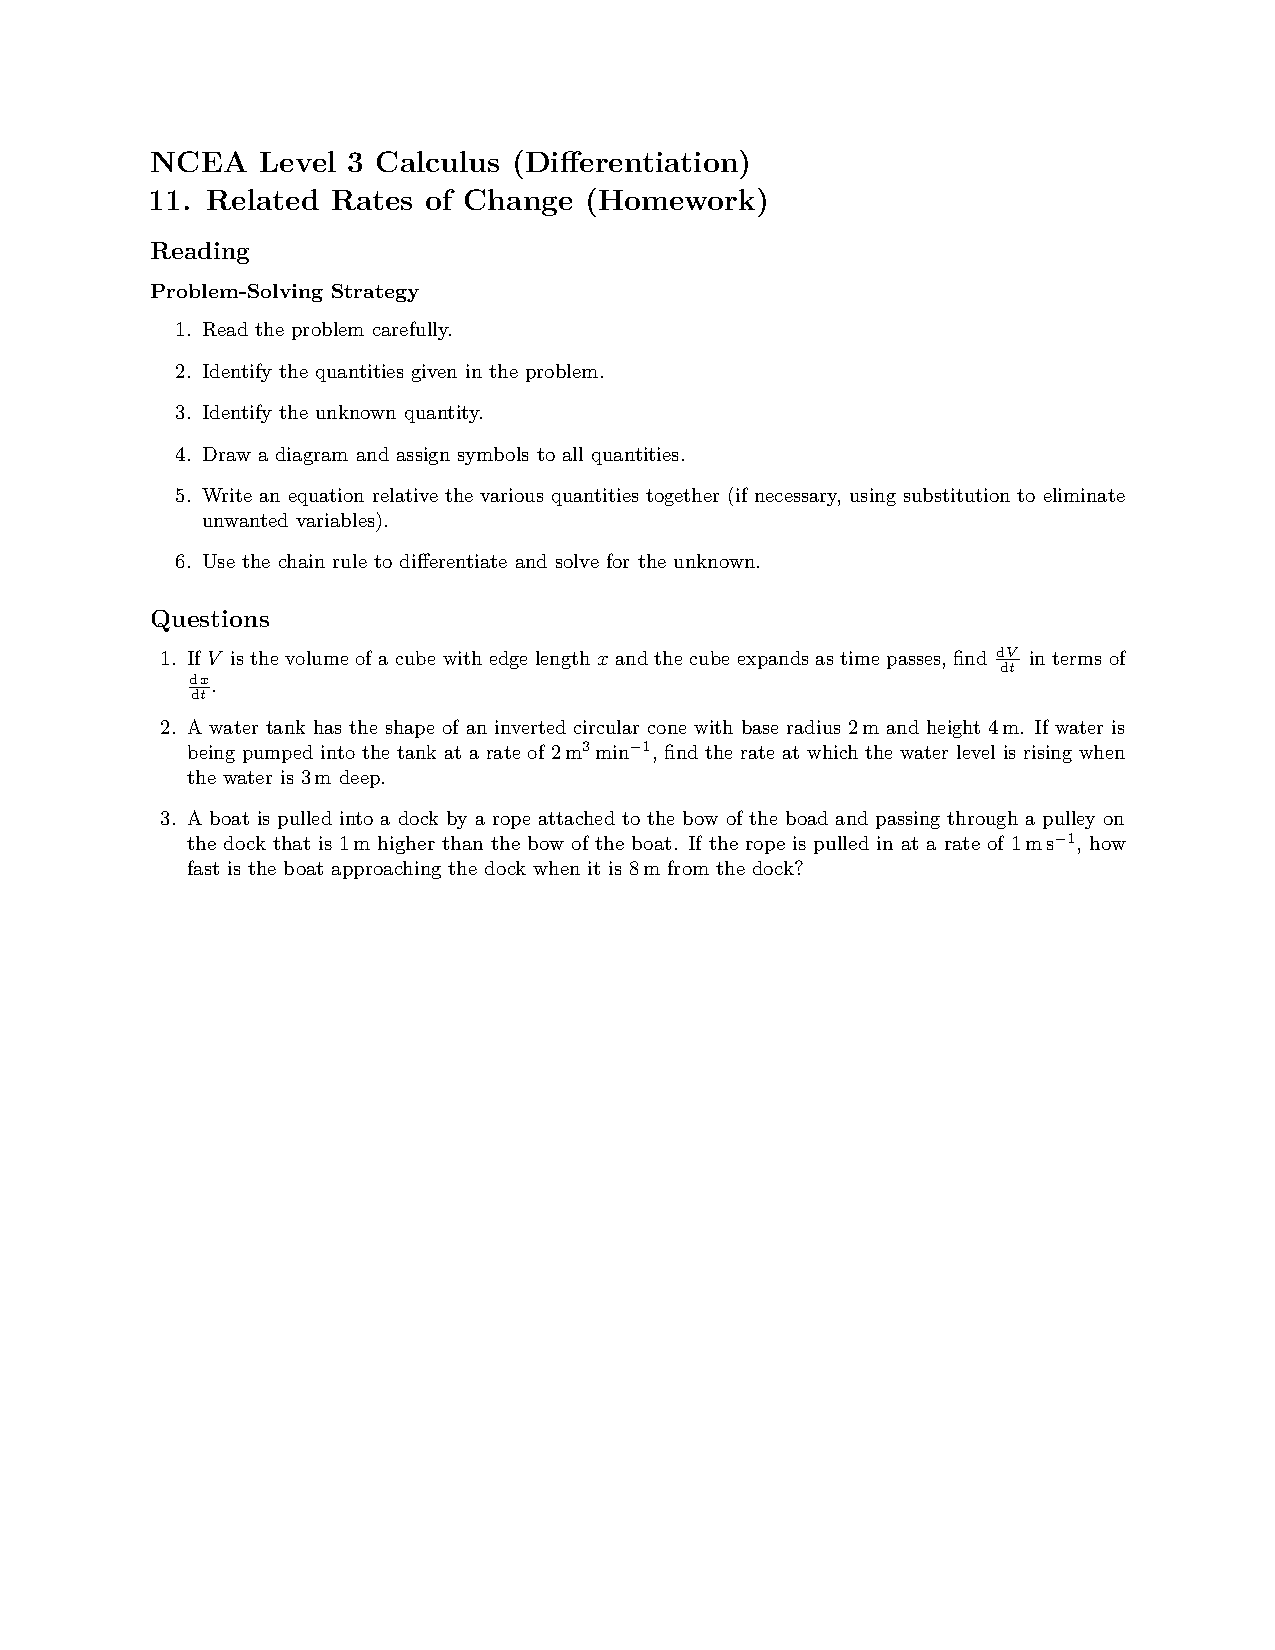
\includepdf[pages={-},pagecommand={}]{11-chainrule2-hw.pdf}
  \phantomsection\addcontentsline{toc}{section}{12. Parametric Functions}
  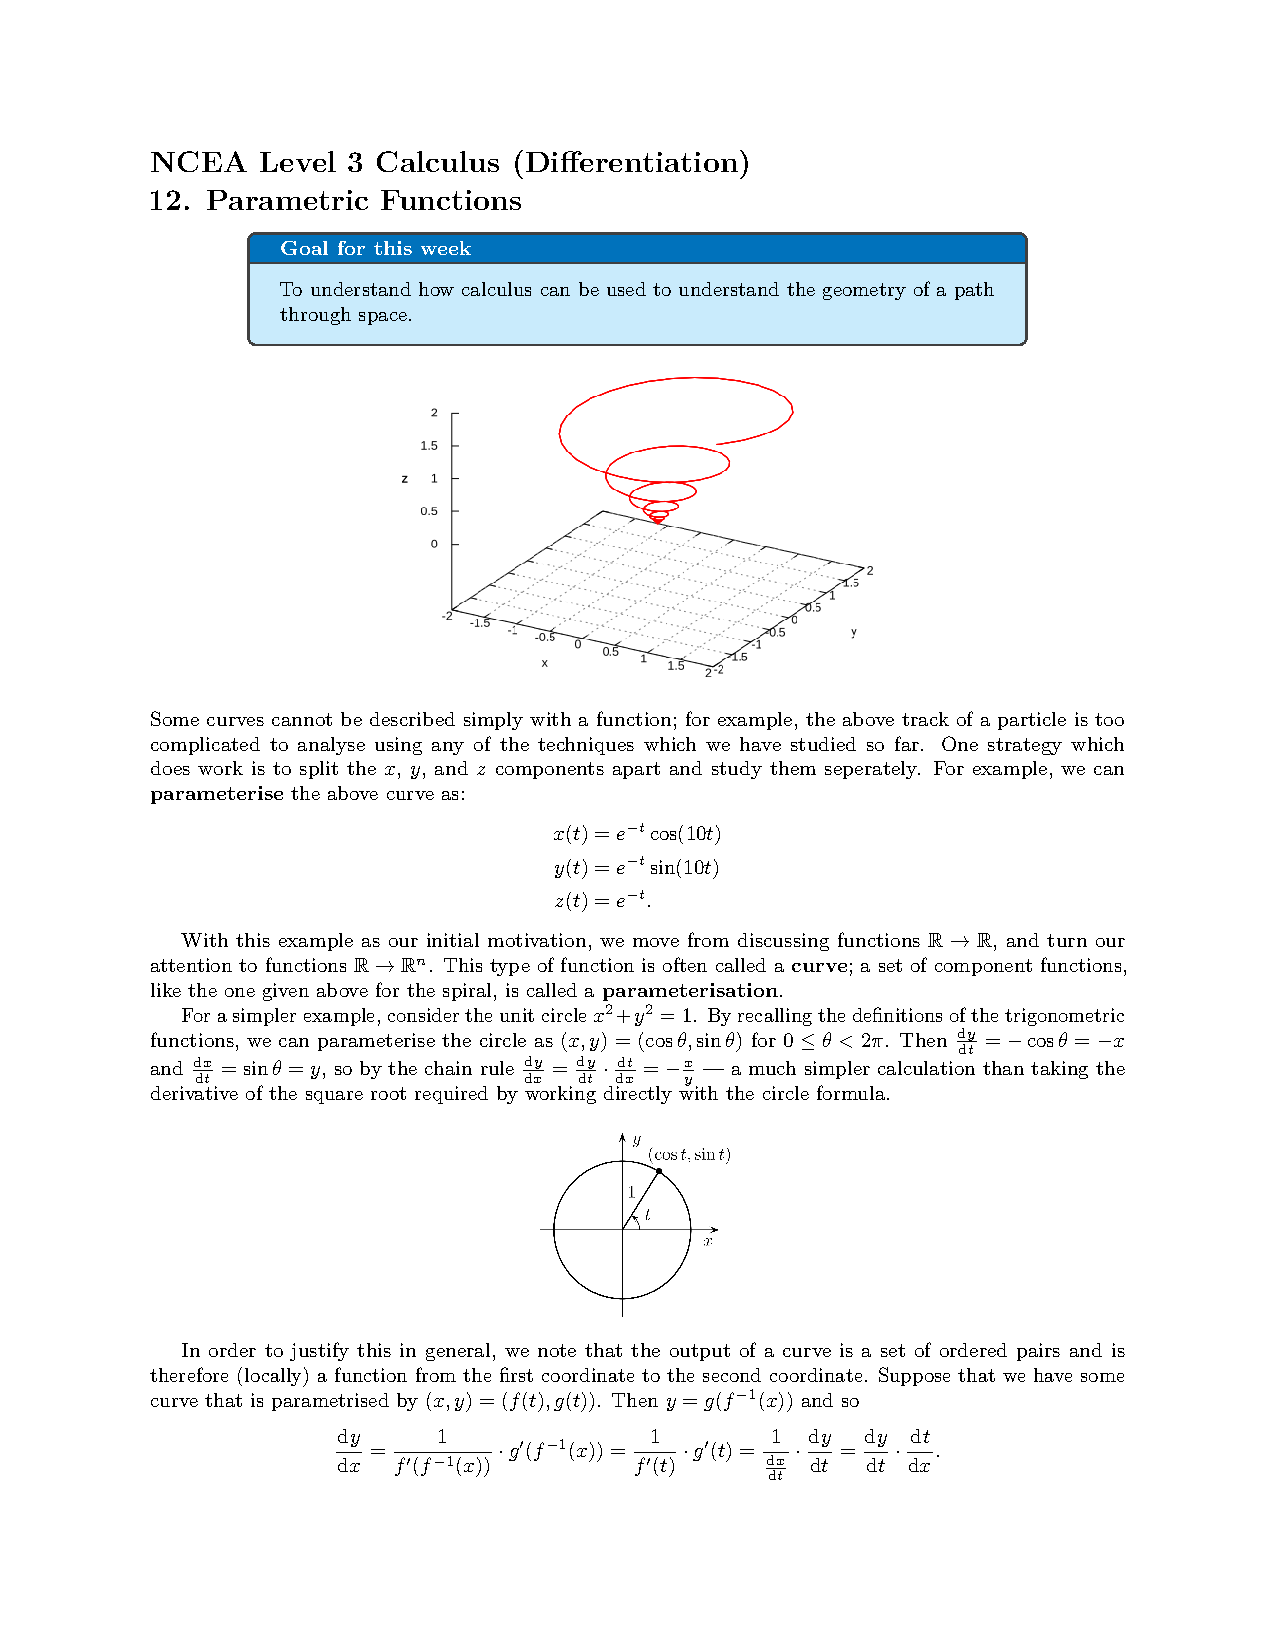
\includepdf[pages={-},pagecommand={}]{12-parametric.pdf}
  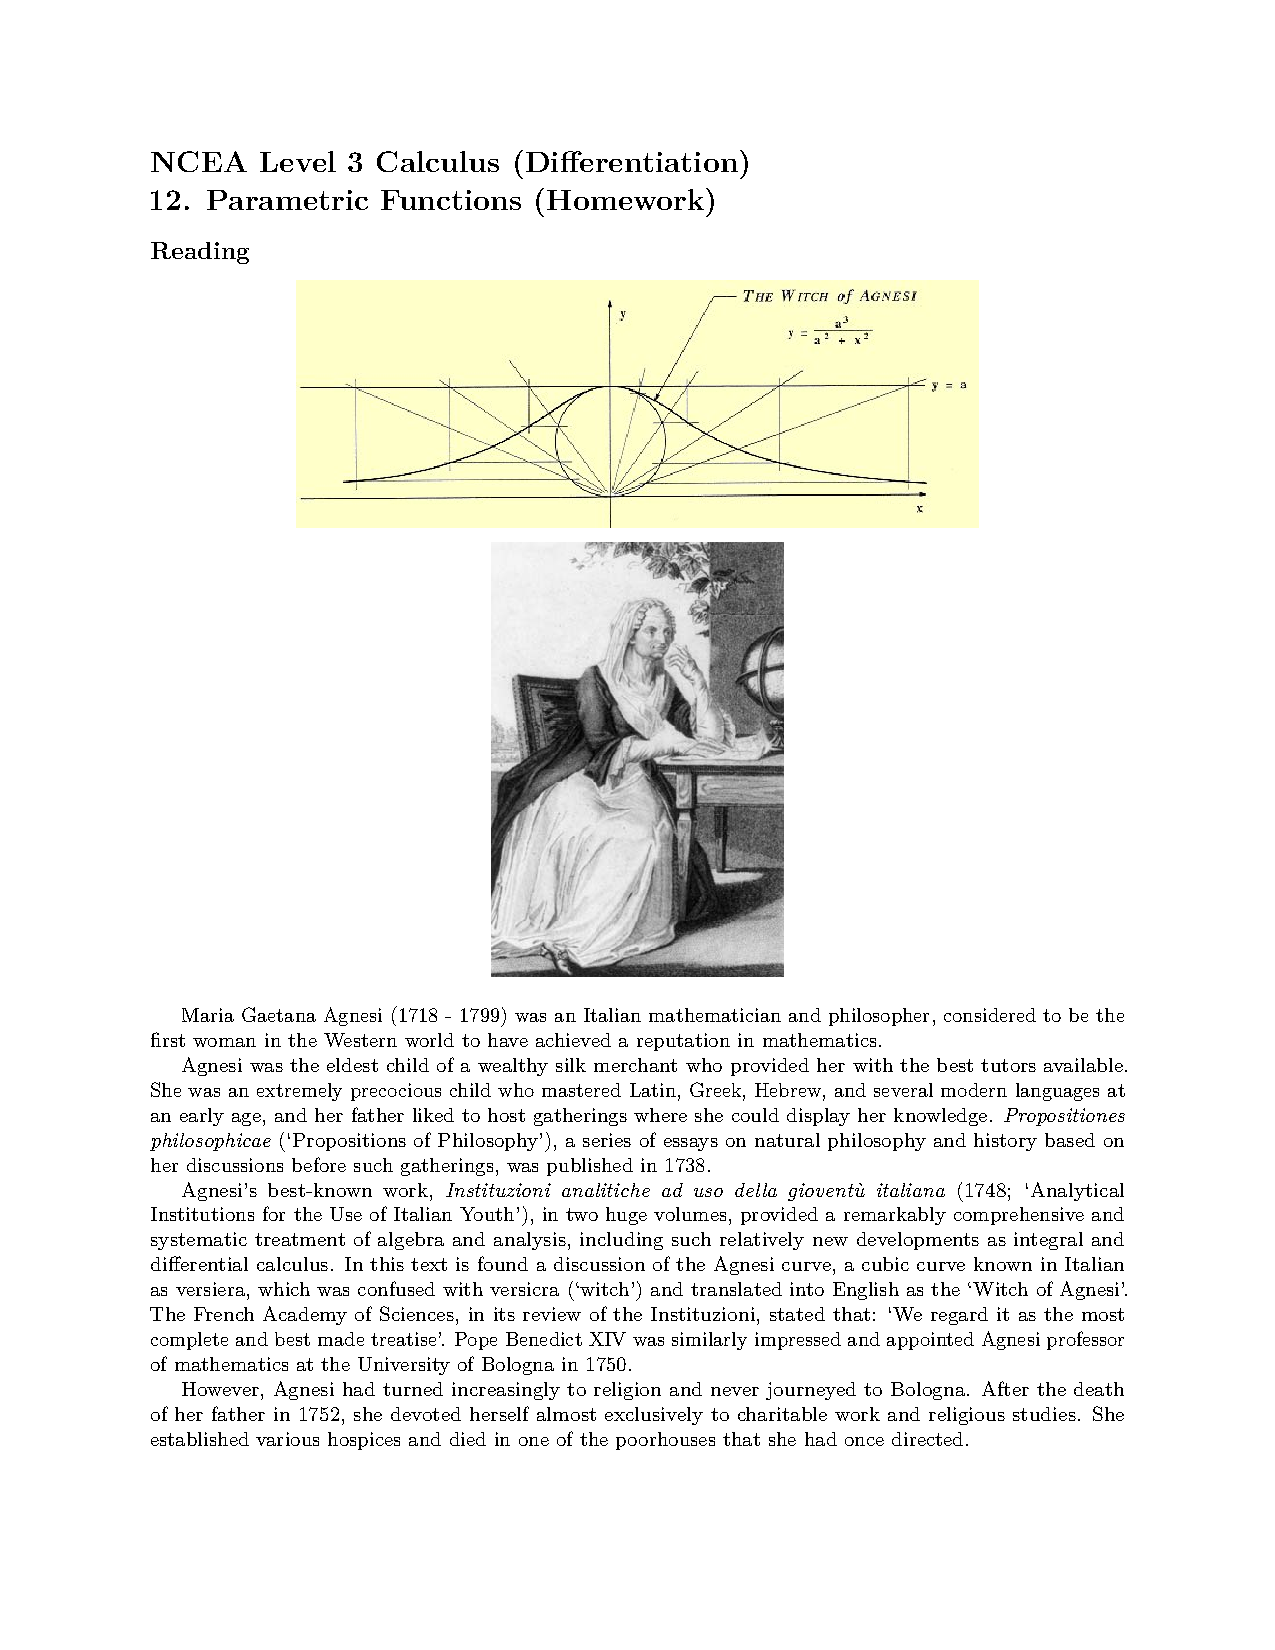
\includepdf[pages={-},pagecommand={}]{12-parametric-hw.pdf}
  \phantomsection\addcontentsline{toc}{section}{13. Sequences and Series}
  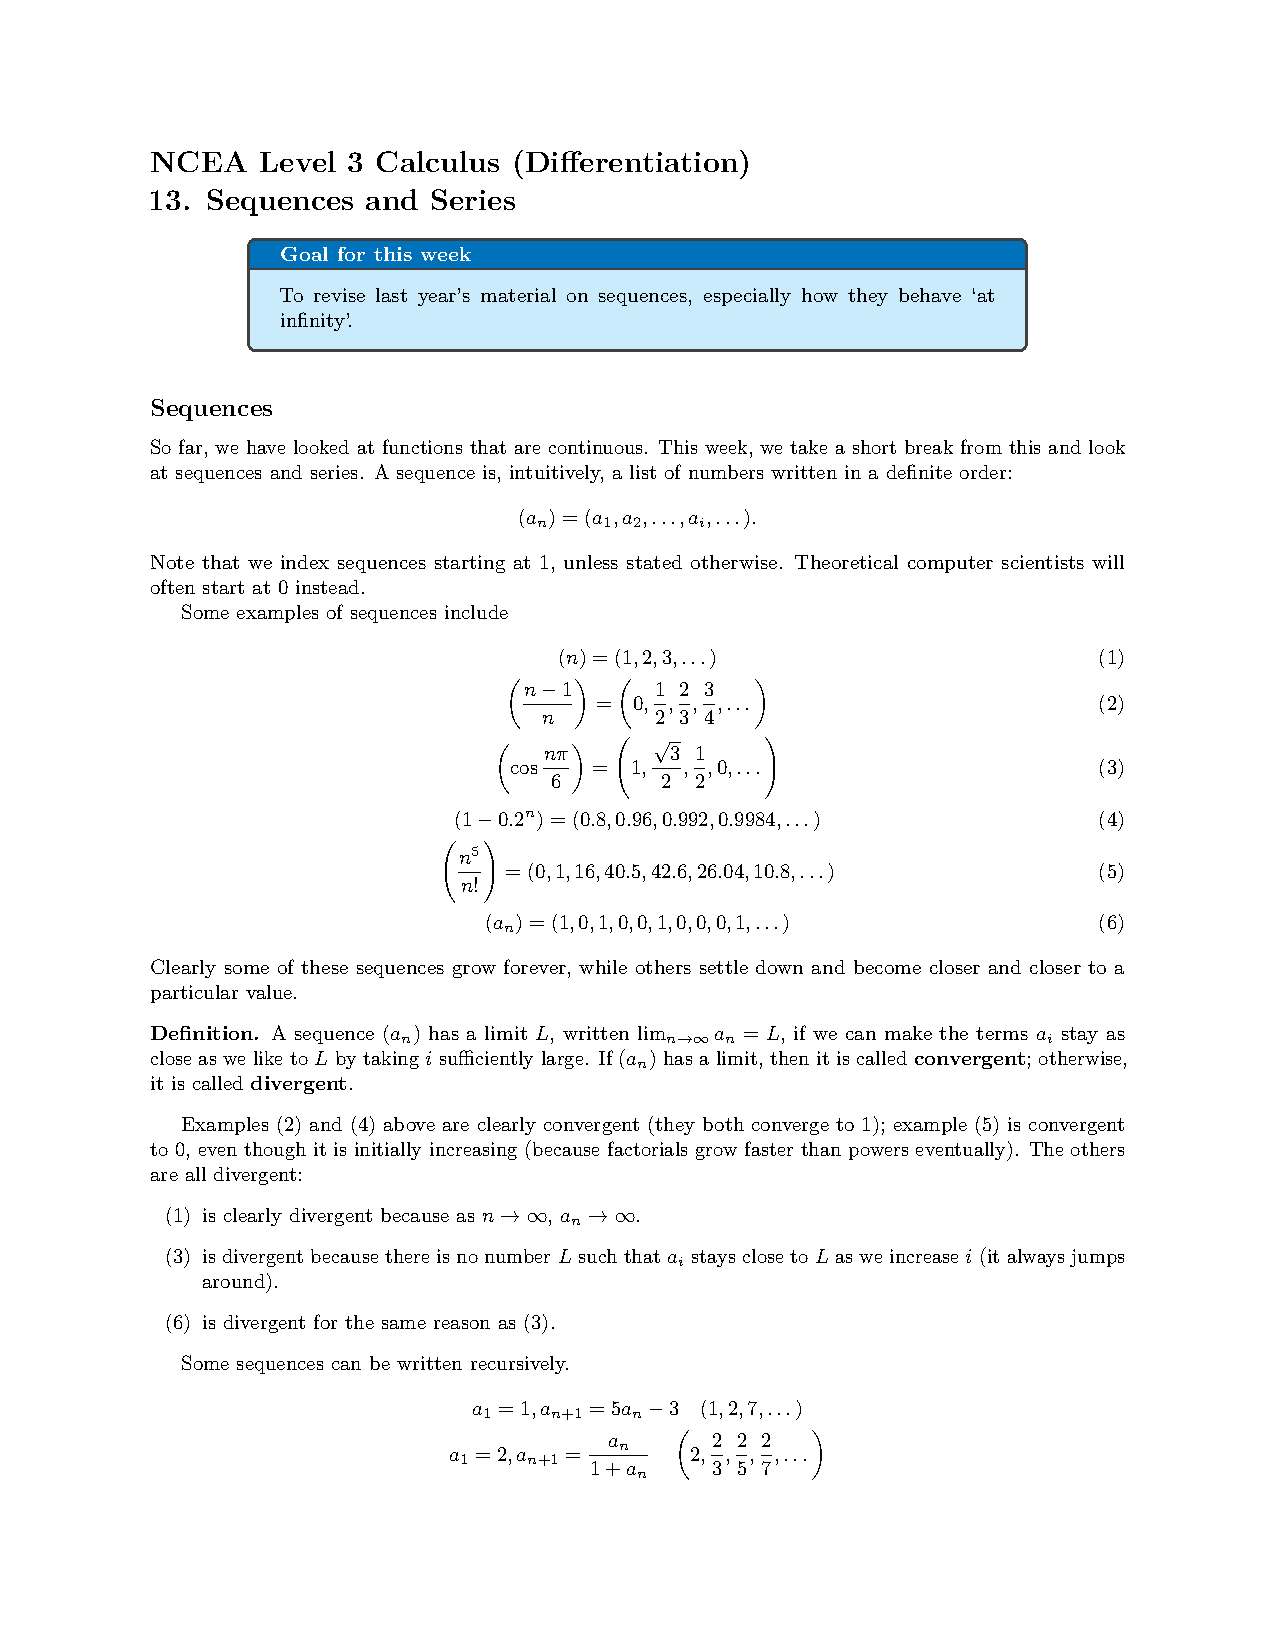
\includepdf[pages={-},pagecommand={}]{13-sequences.pdf}
  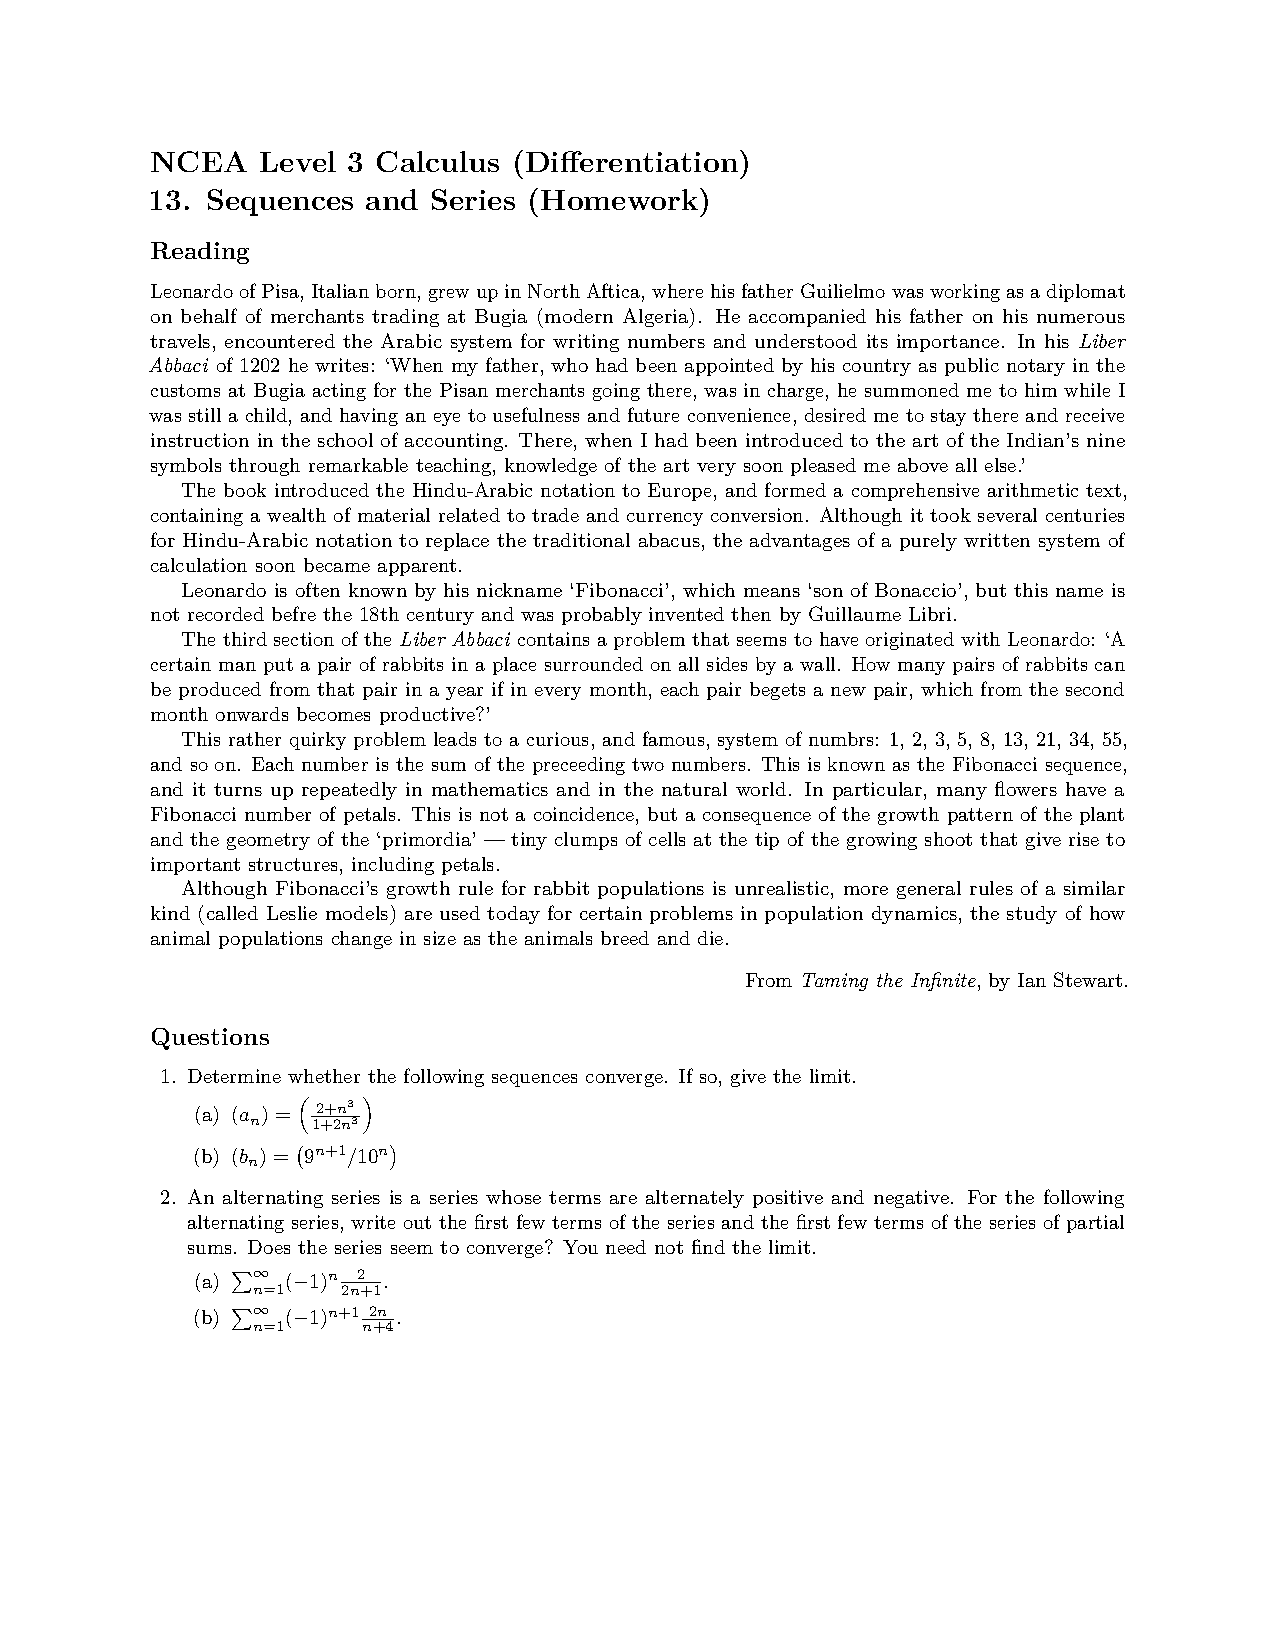
\includepdf[pages={-},pagecommand={}]{13-sequences-hw.pdf}
  \phantomsection\addcontentsline{toc}{section}{14. Differentiation Revision}
  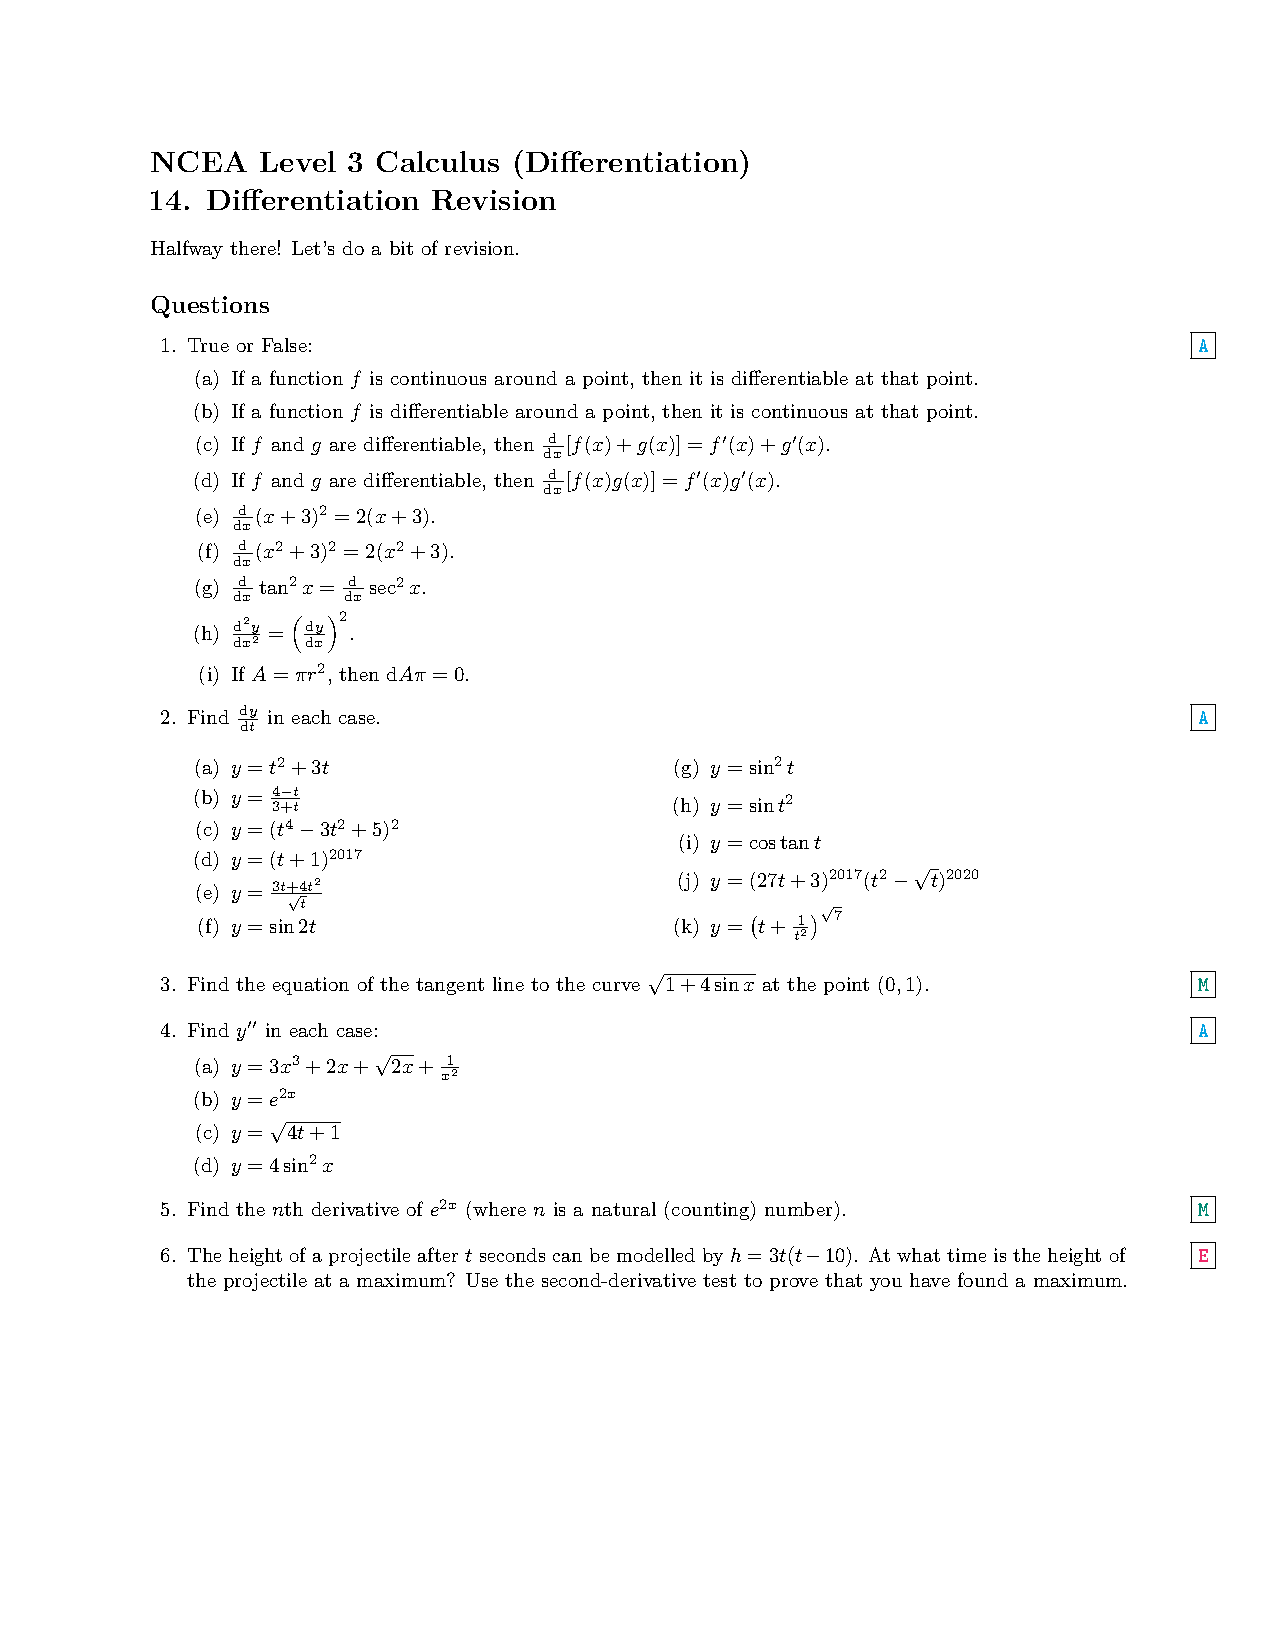
\includepdf[pages={-},pagecommand={}]{14-diffrev.pdf}
  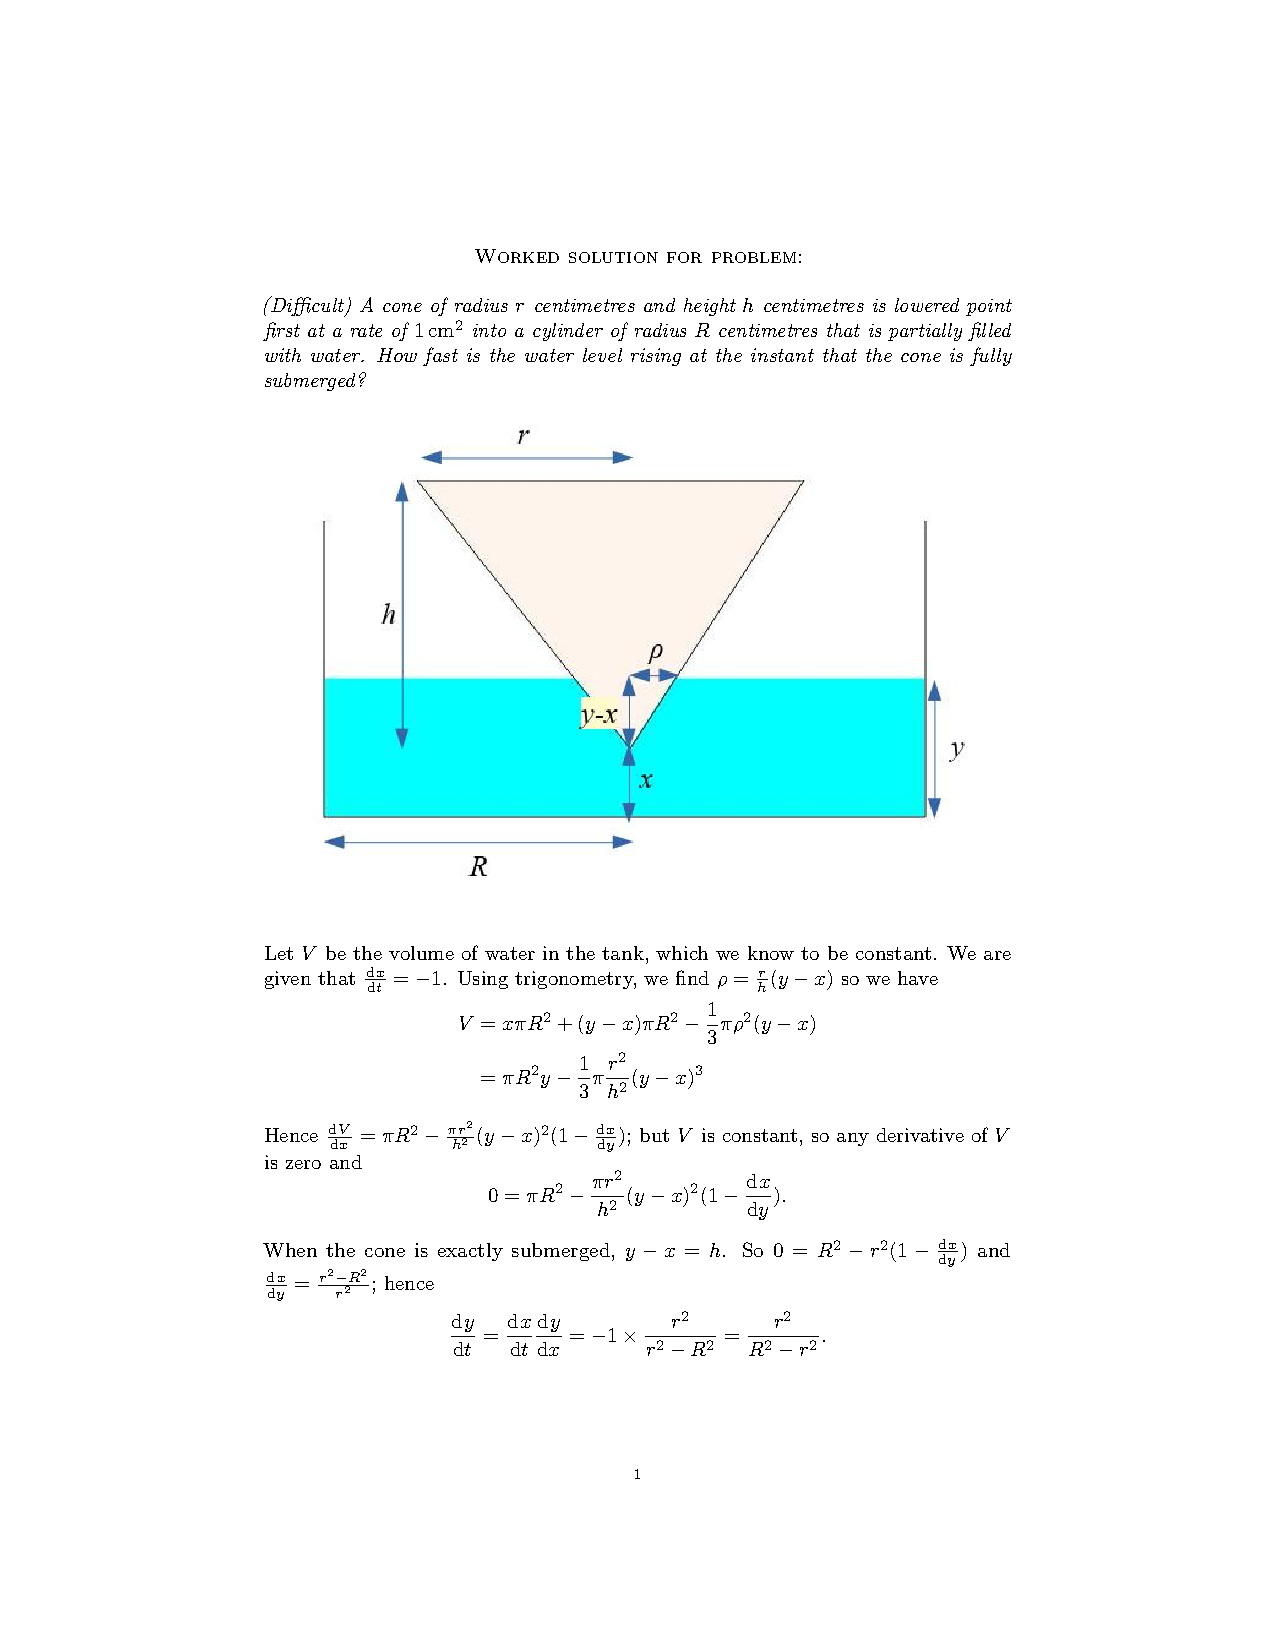
\includepdf[pages={-},pagecommand={}]{14a-workedsol-cone.pdf}
  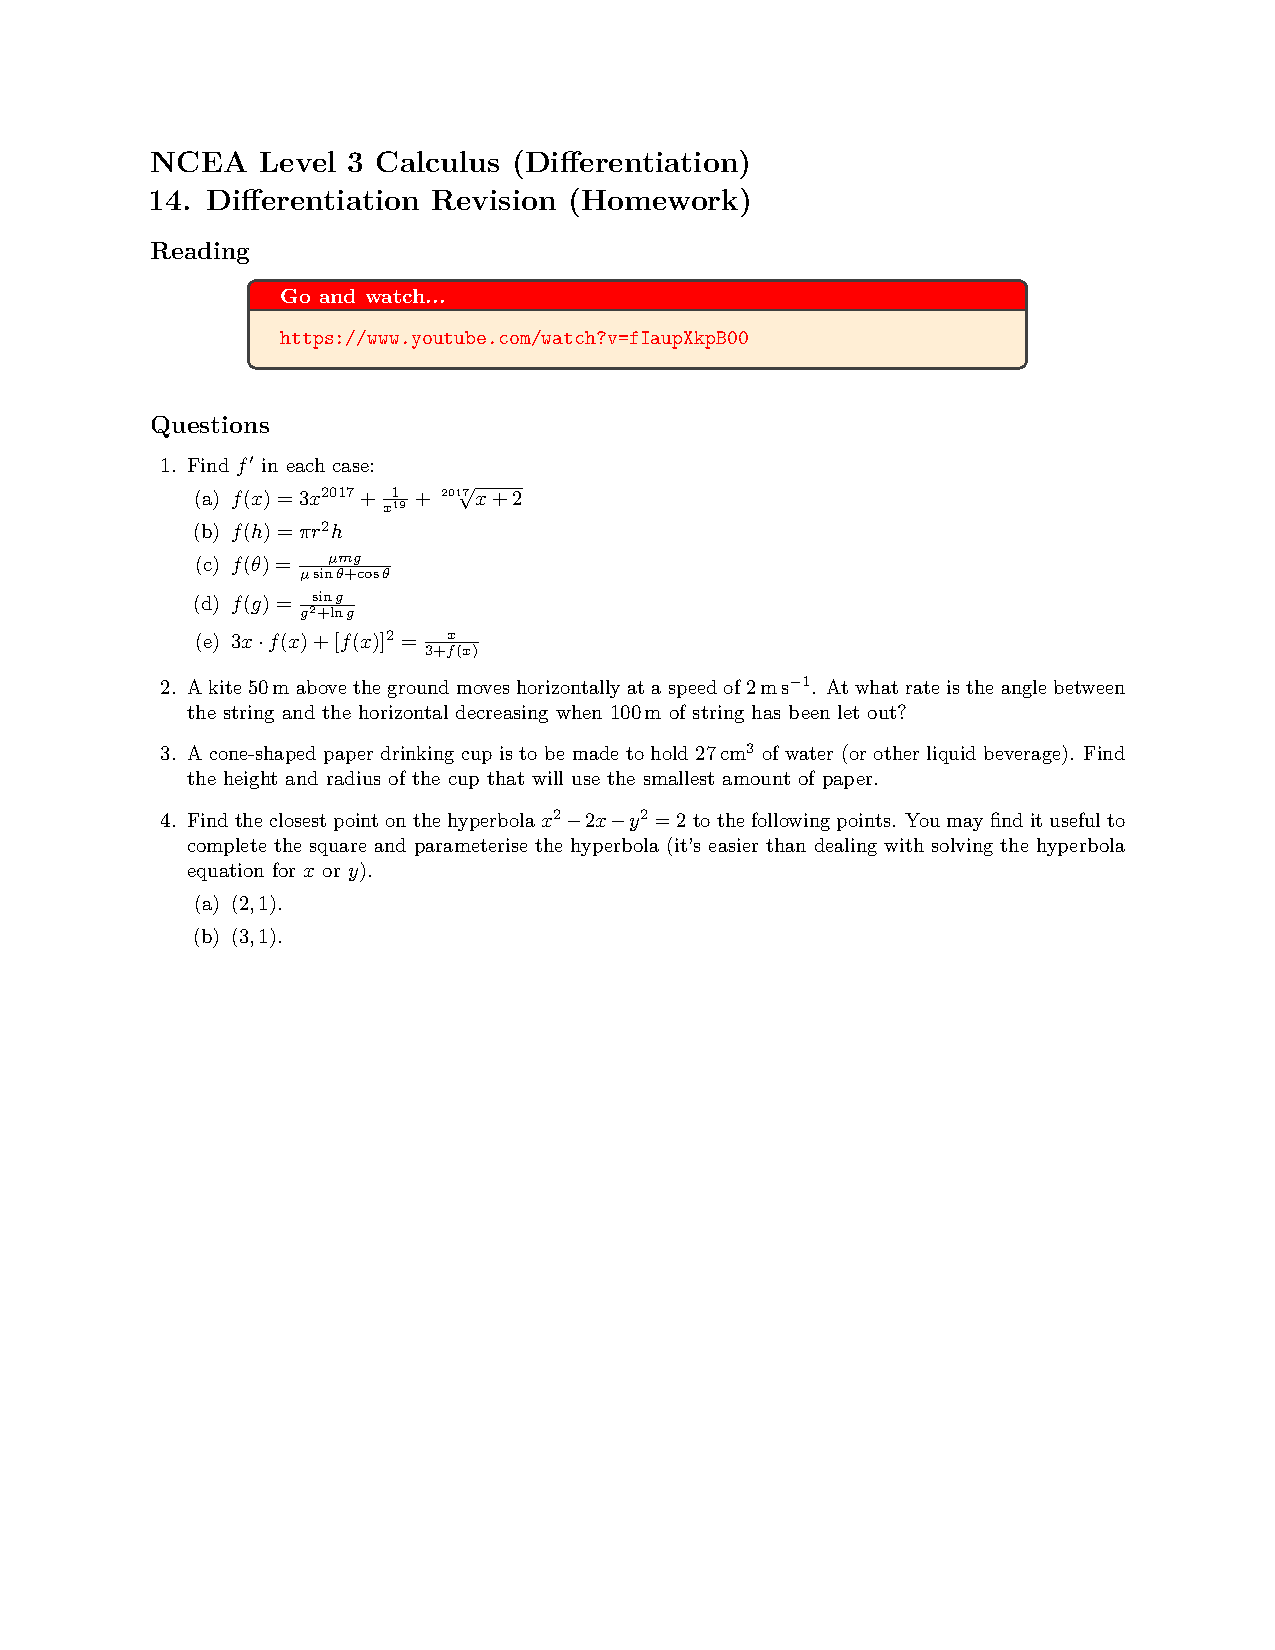
\includepdf[pages={-},pagecommand={}]{14-diffrev-hw.pdf}

  \chapter{Integration}
  \phantomsection\addcontentsline{toc}{section}{15. Approximating Areas}
  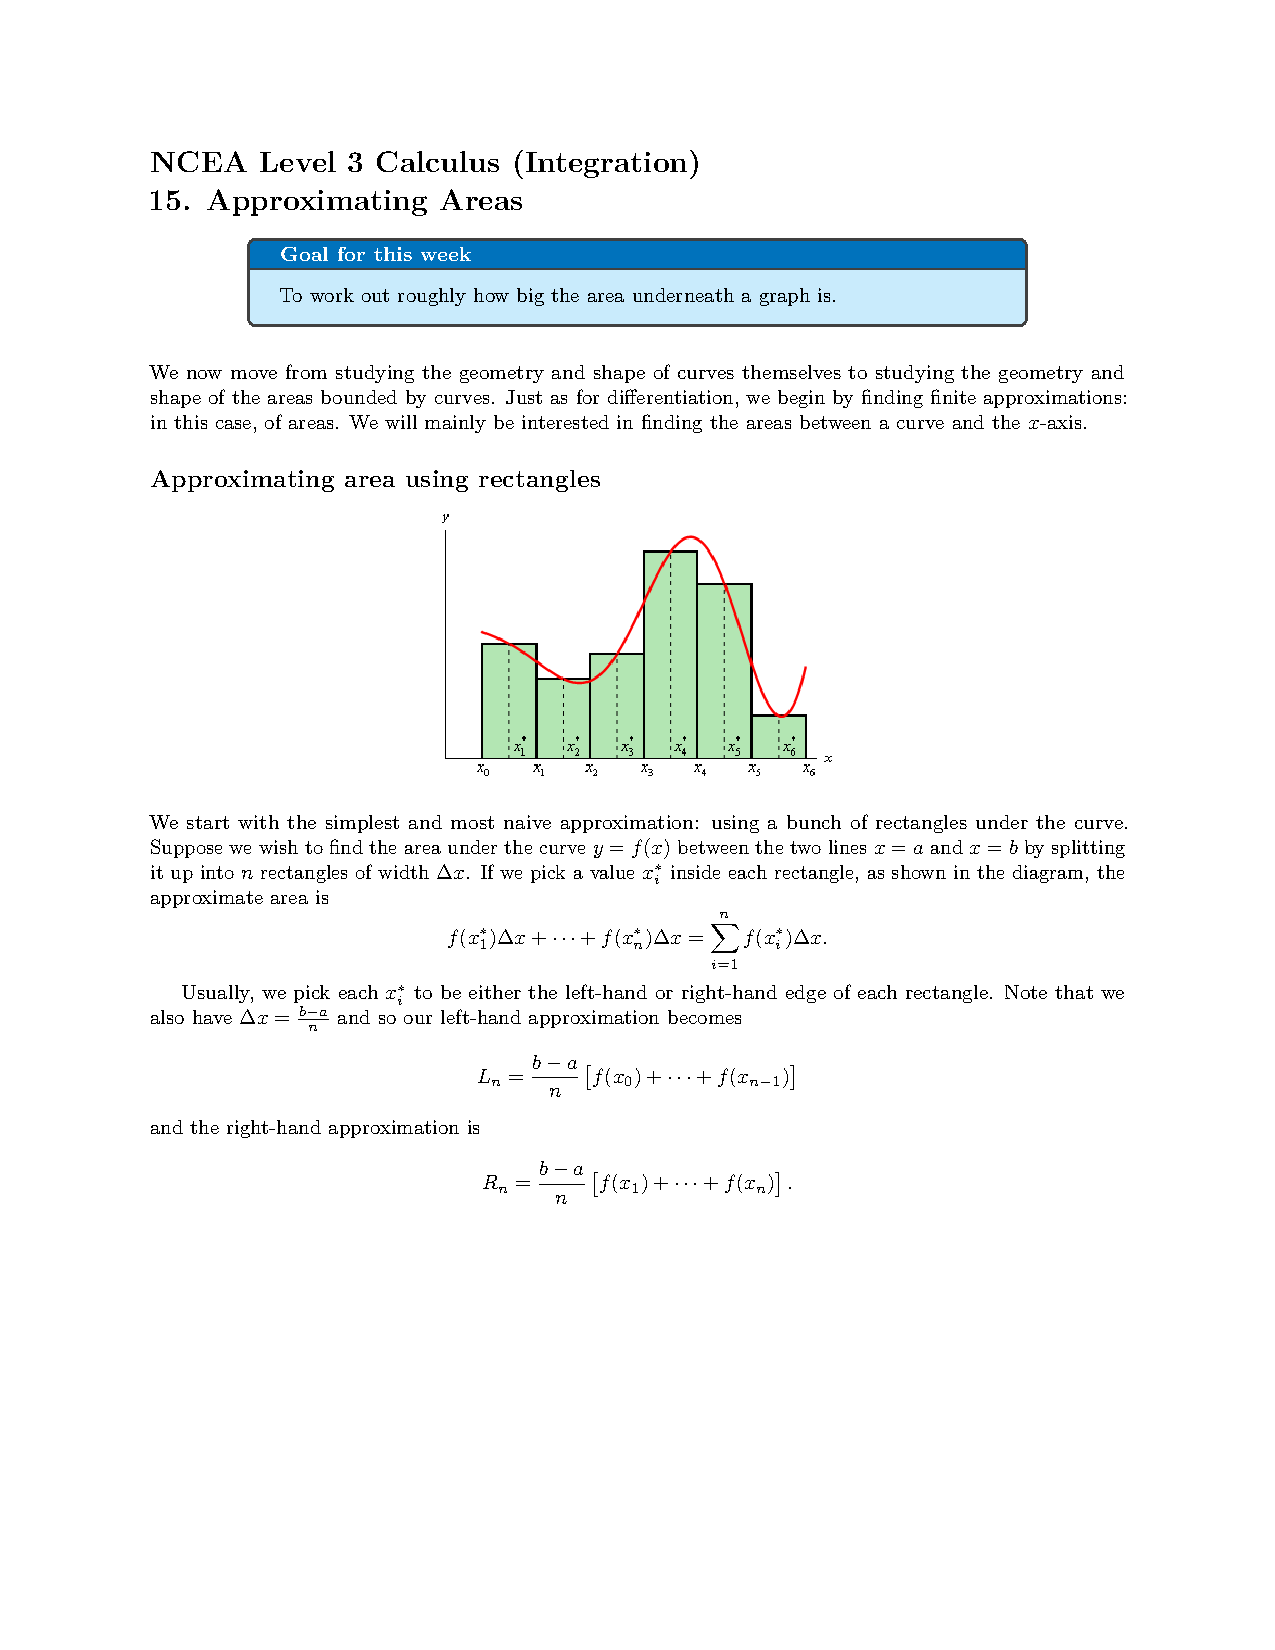
\includepdf[pages={-},pagecommand={}]{15-approximatingareas.pdf}
  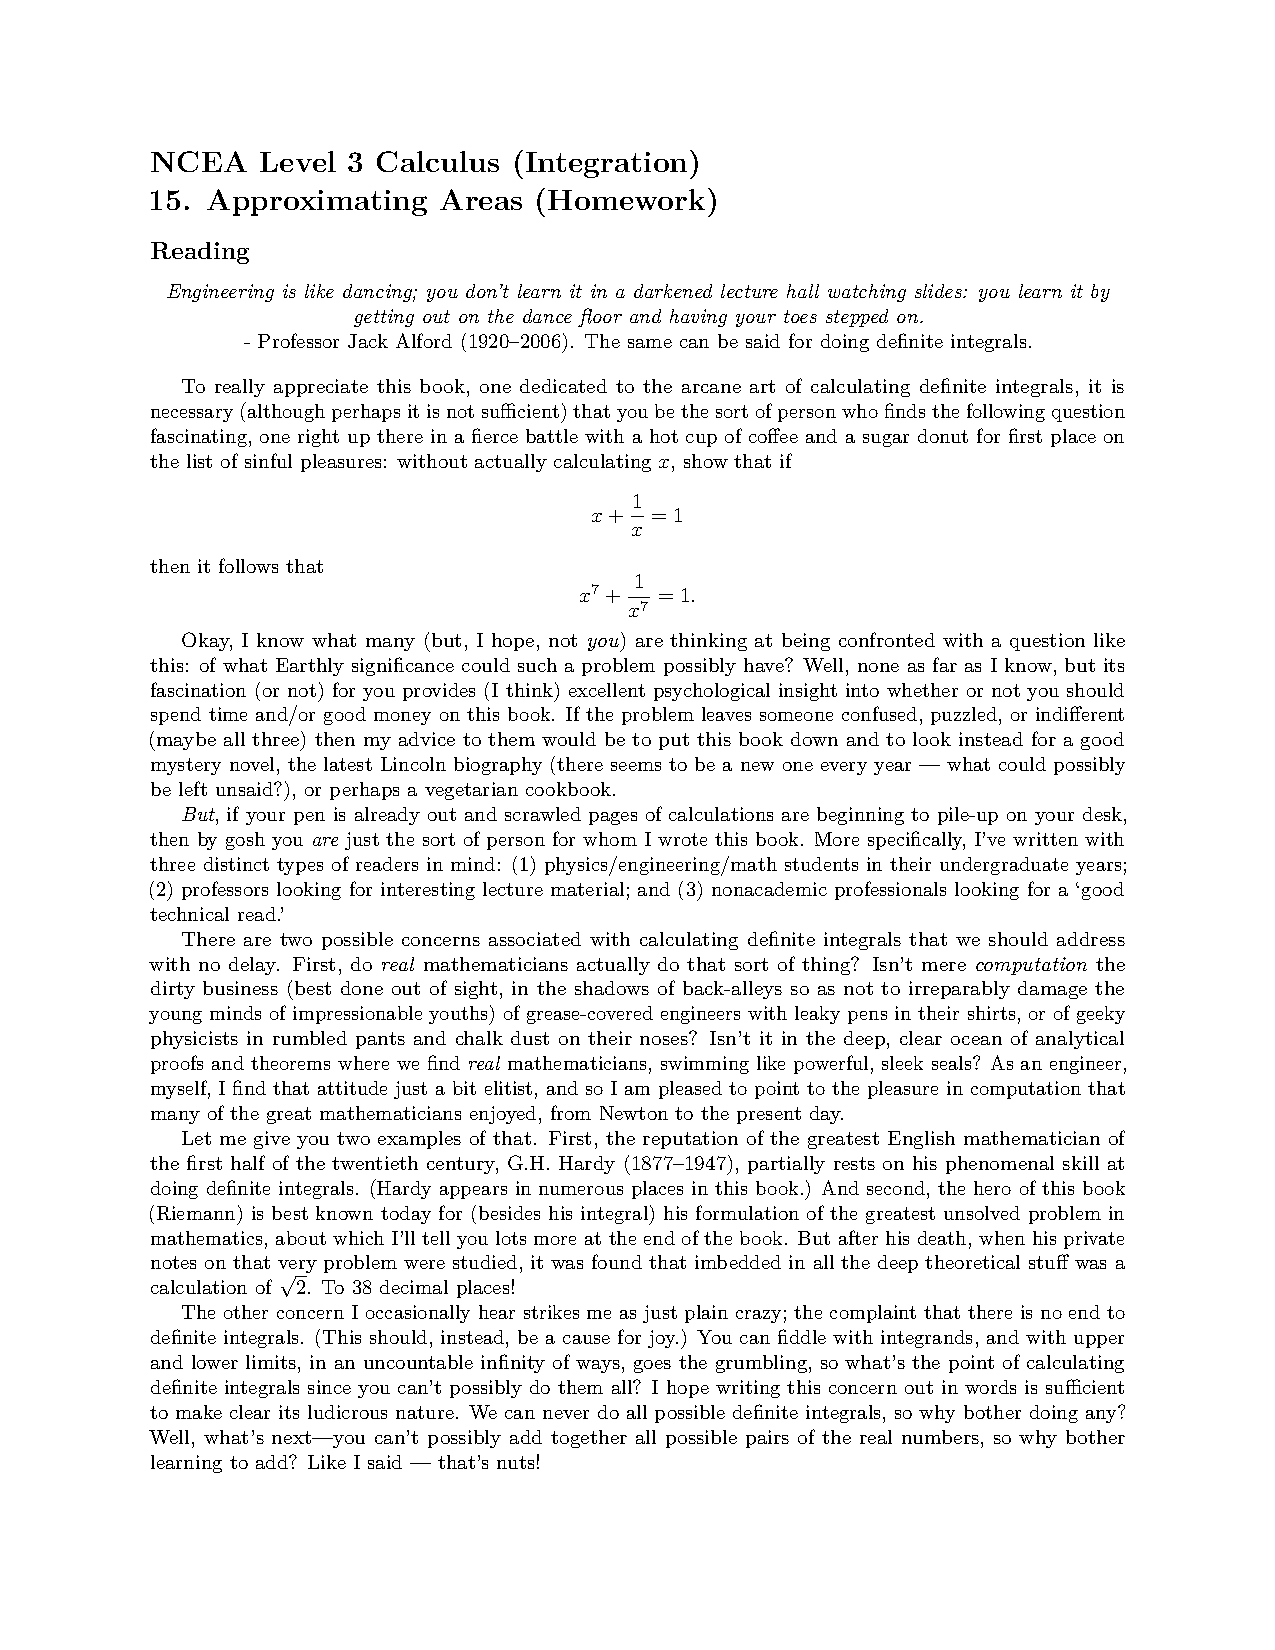
\includepdf[pages={-},pagecommand={}]{15-approximatingareas-hw.pdf}
  \phantomsection\addcontentsline{toc}{section}{16. Anti-differentiation}
  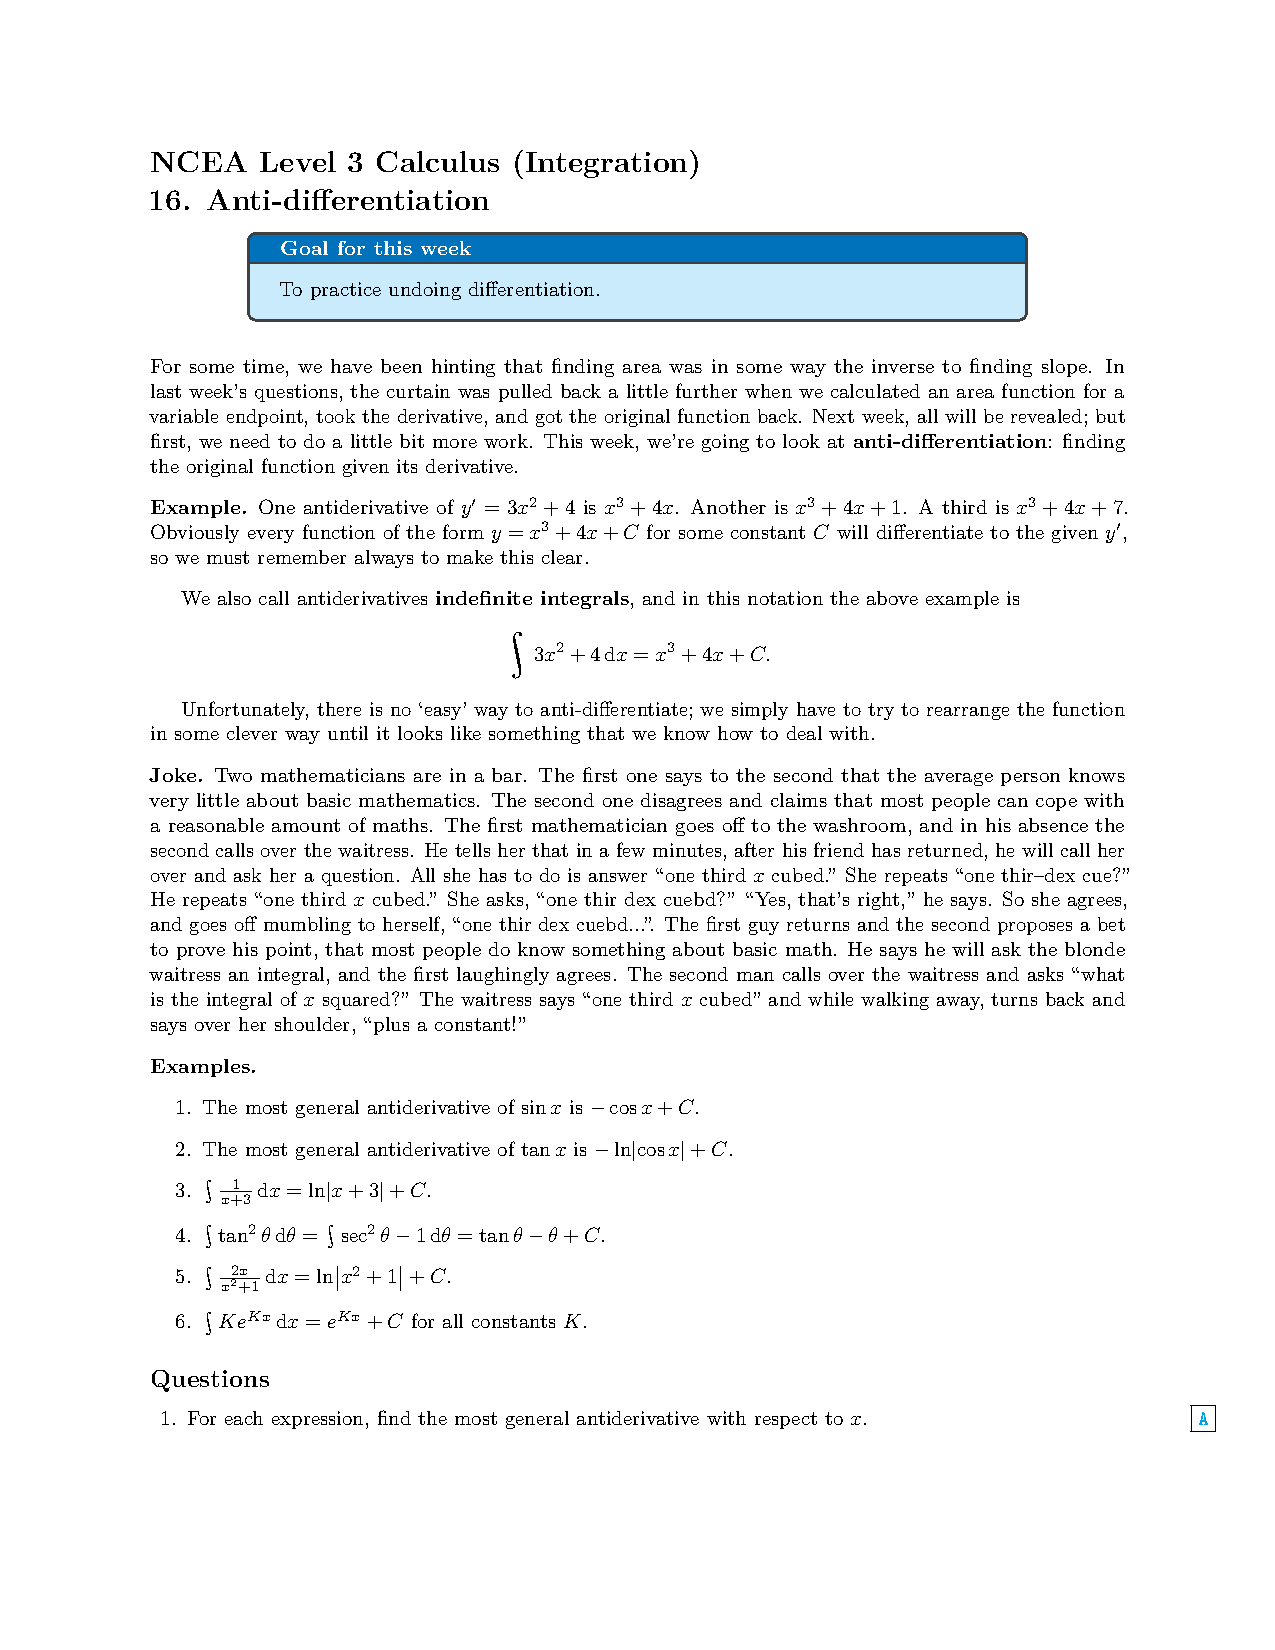
\includepdf[pages={-},pagecommand={}]{16-antidifferentiation.pdf}
  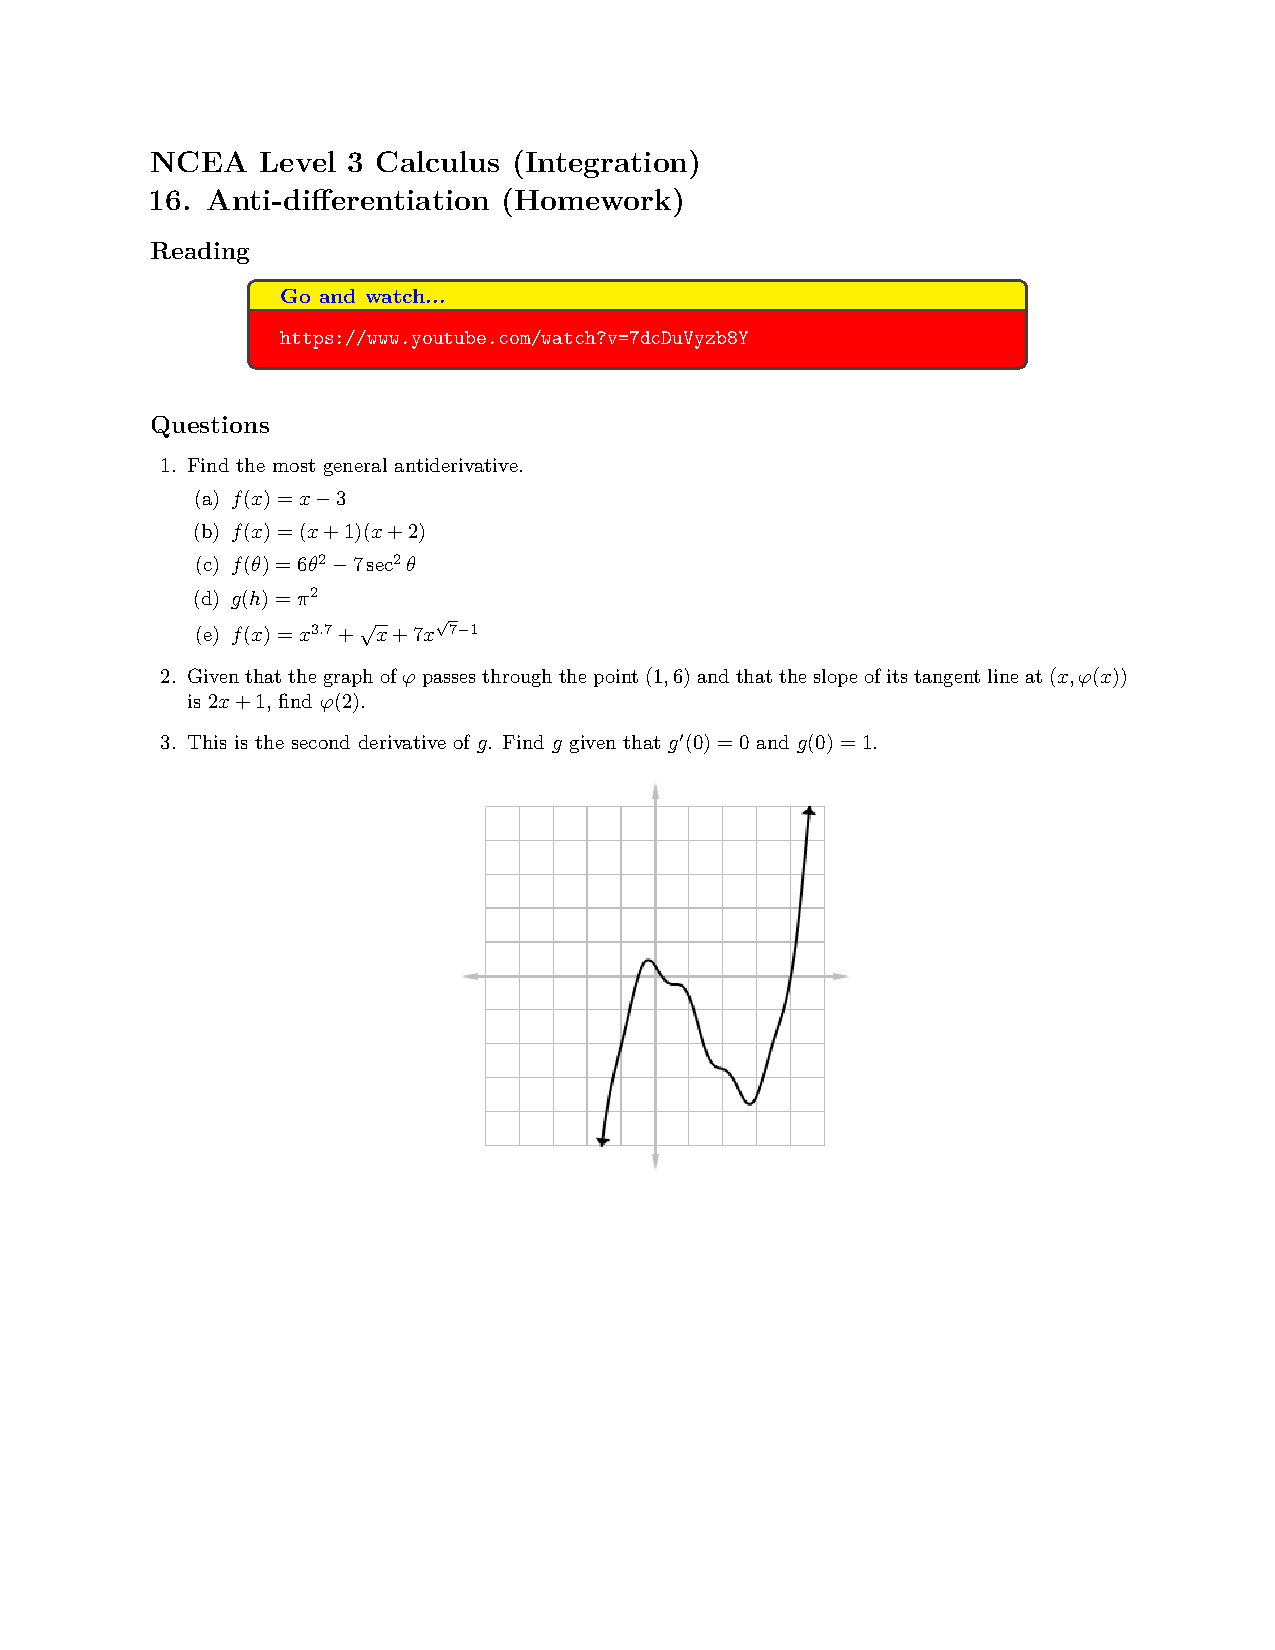
\includepdf[pages={-},pagecommand={}]{16-antidifferentiation-hw.pdf}
  \phantomsection\addcontentsline{toc}{section}{17. The Fundamental Theorem of Calculus}
  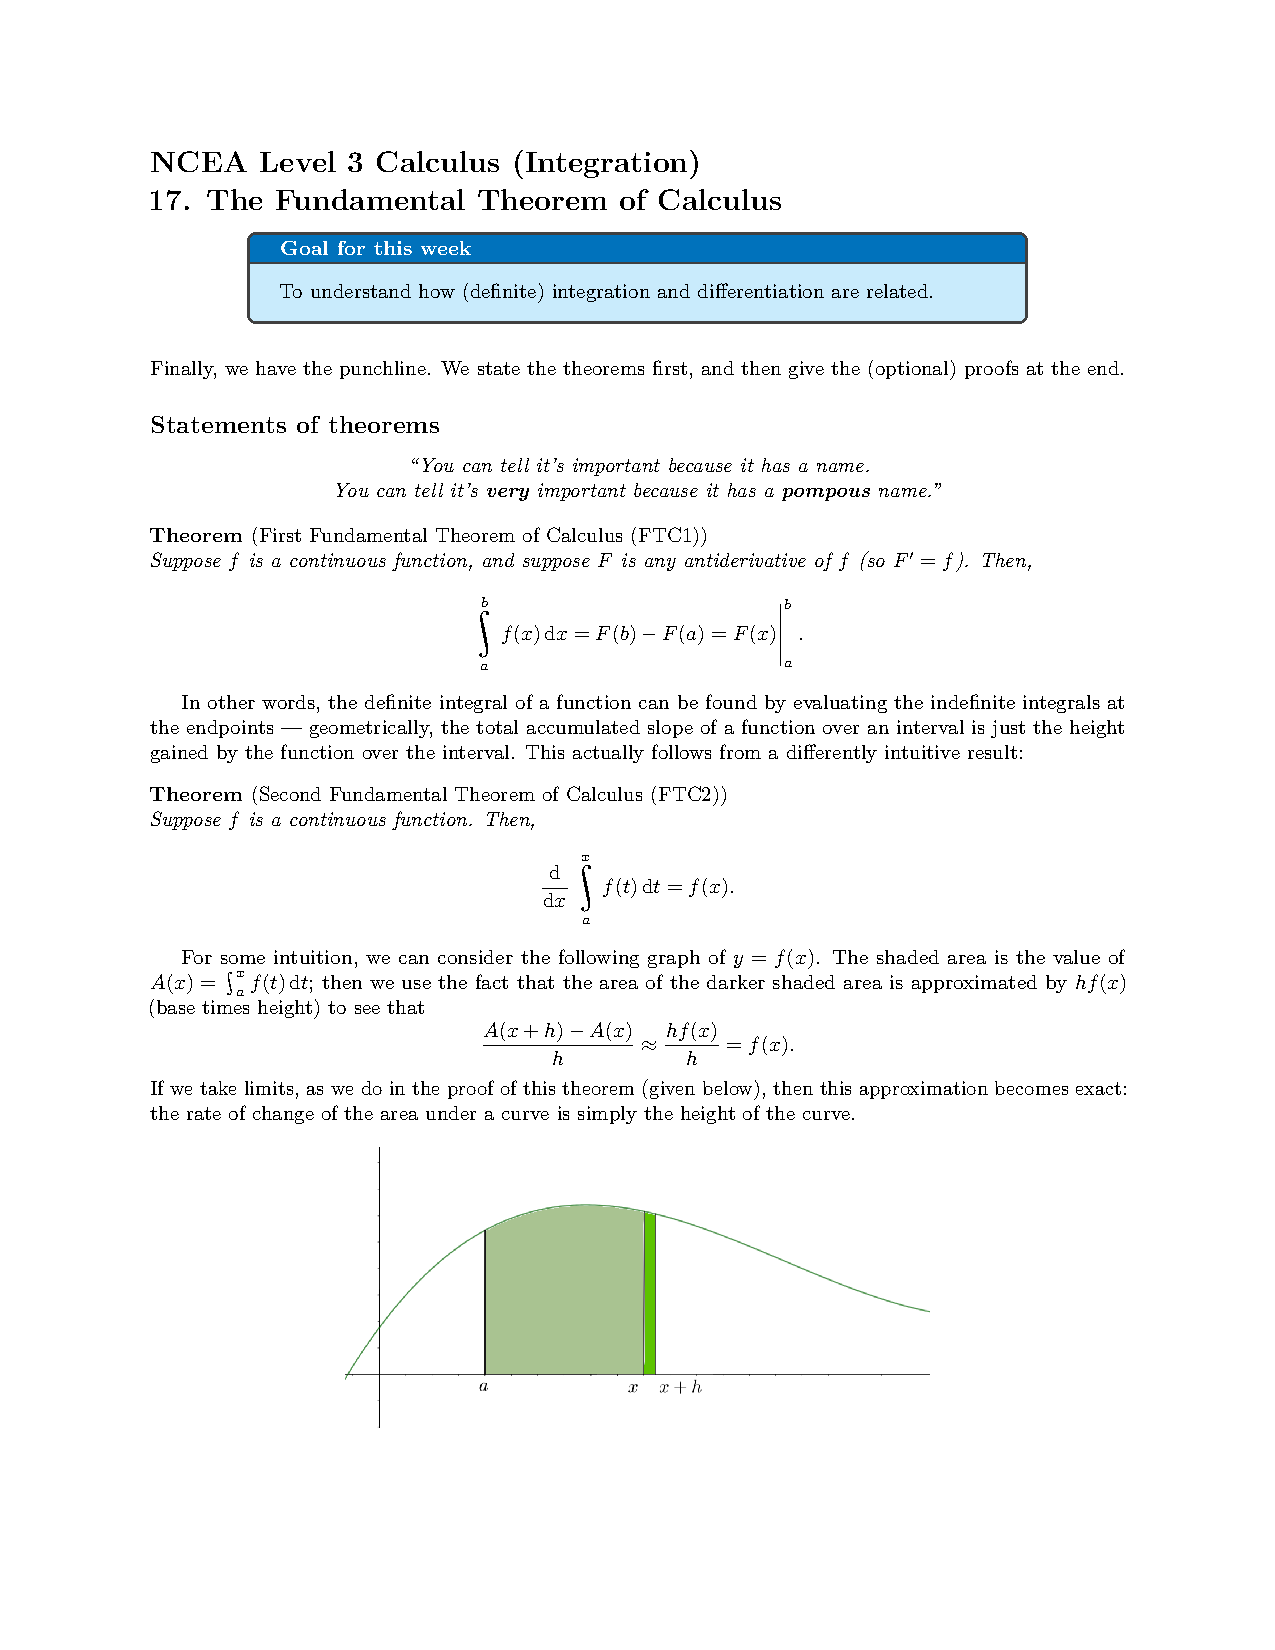
\includepdf[pages={-},pagecommand={}]{17-ftc.pdf}
  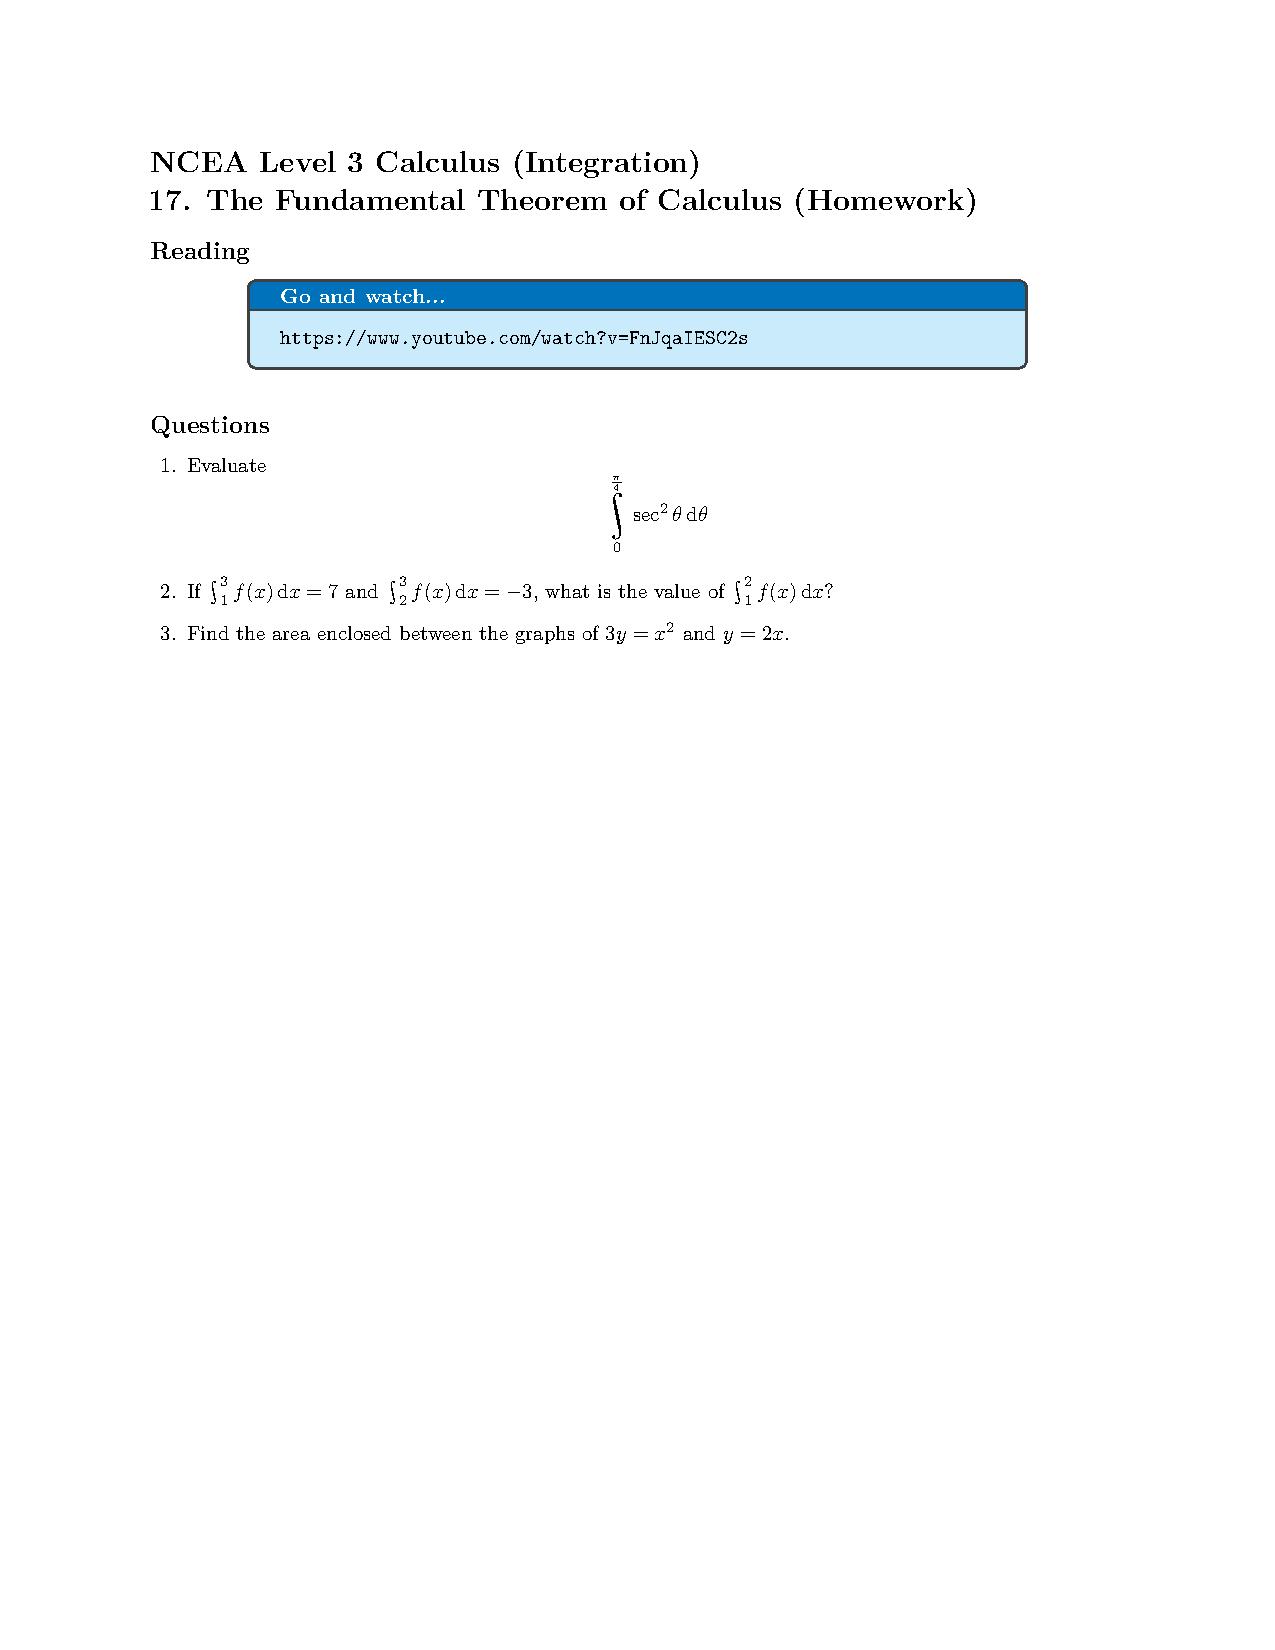
\includepdf[pages={-},pagecommand={}]{17-ftc-hw.pdf}
  \phantomsection\addcontentsline{toc}{section}{18. Substitution}
  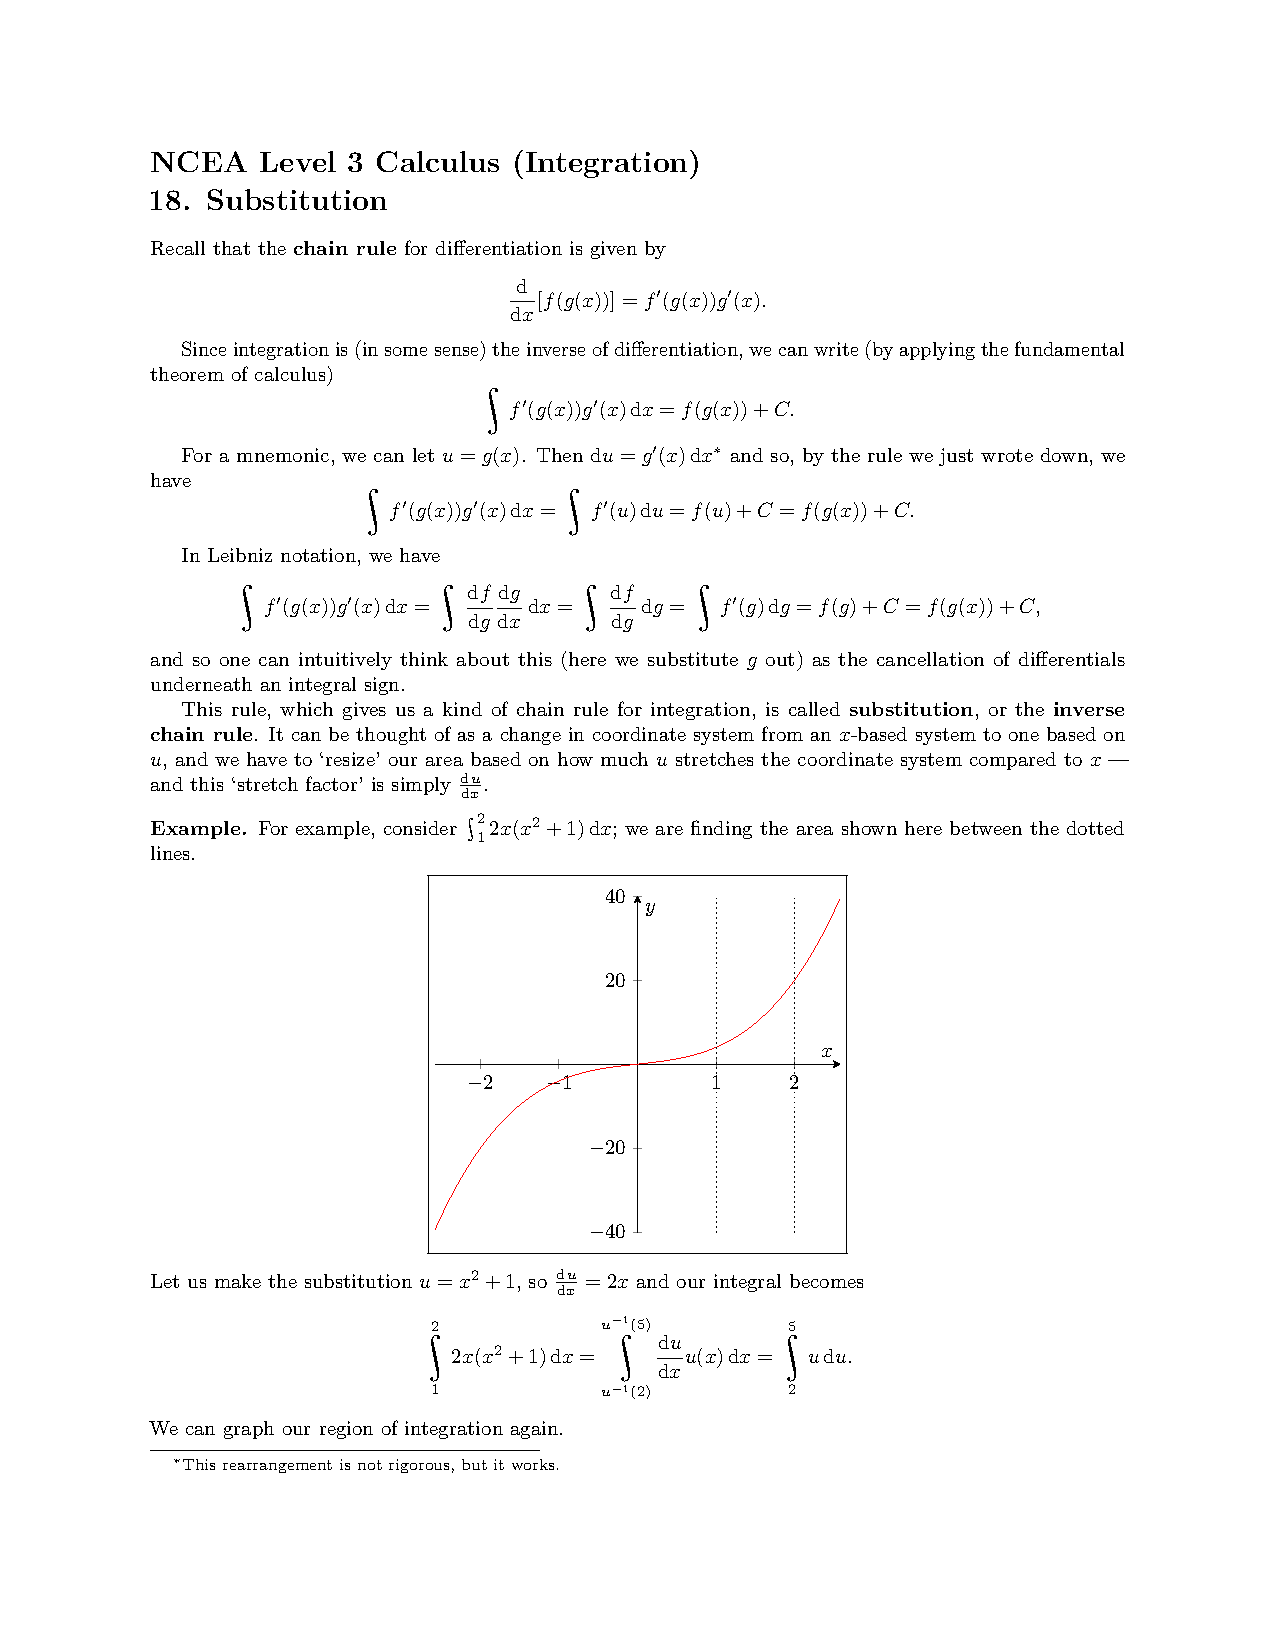
\includepdf[pages={-},pagecommand={}]{18-subsn.pdf}
  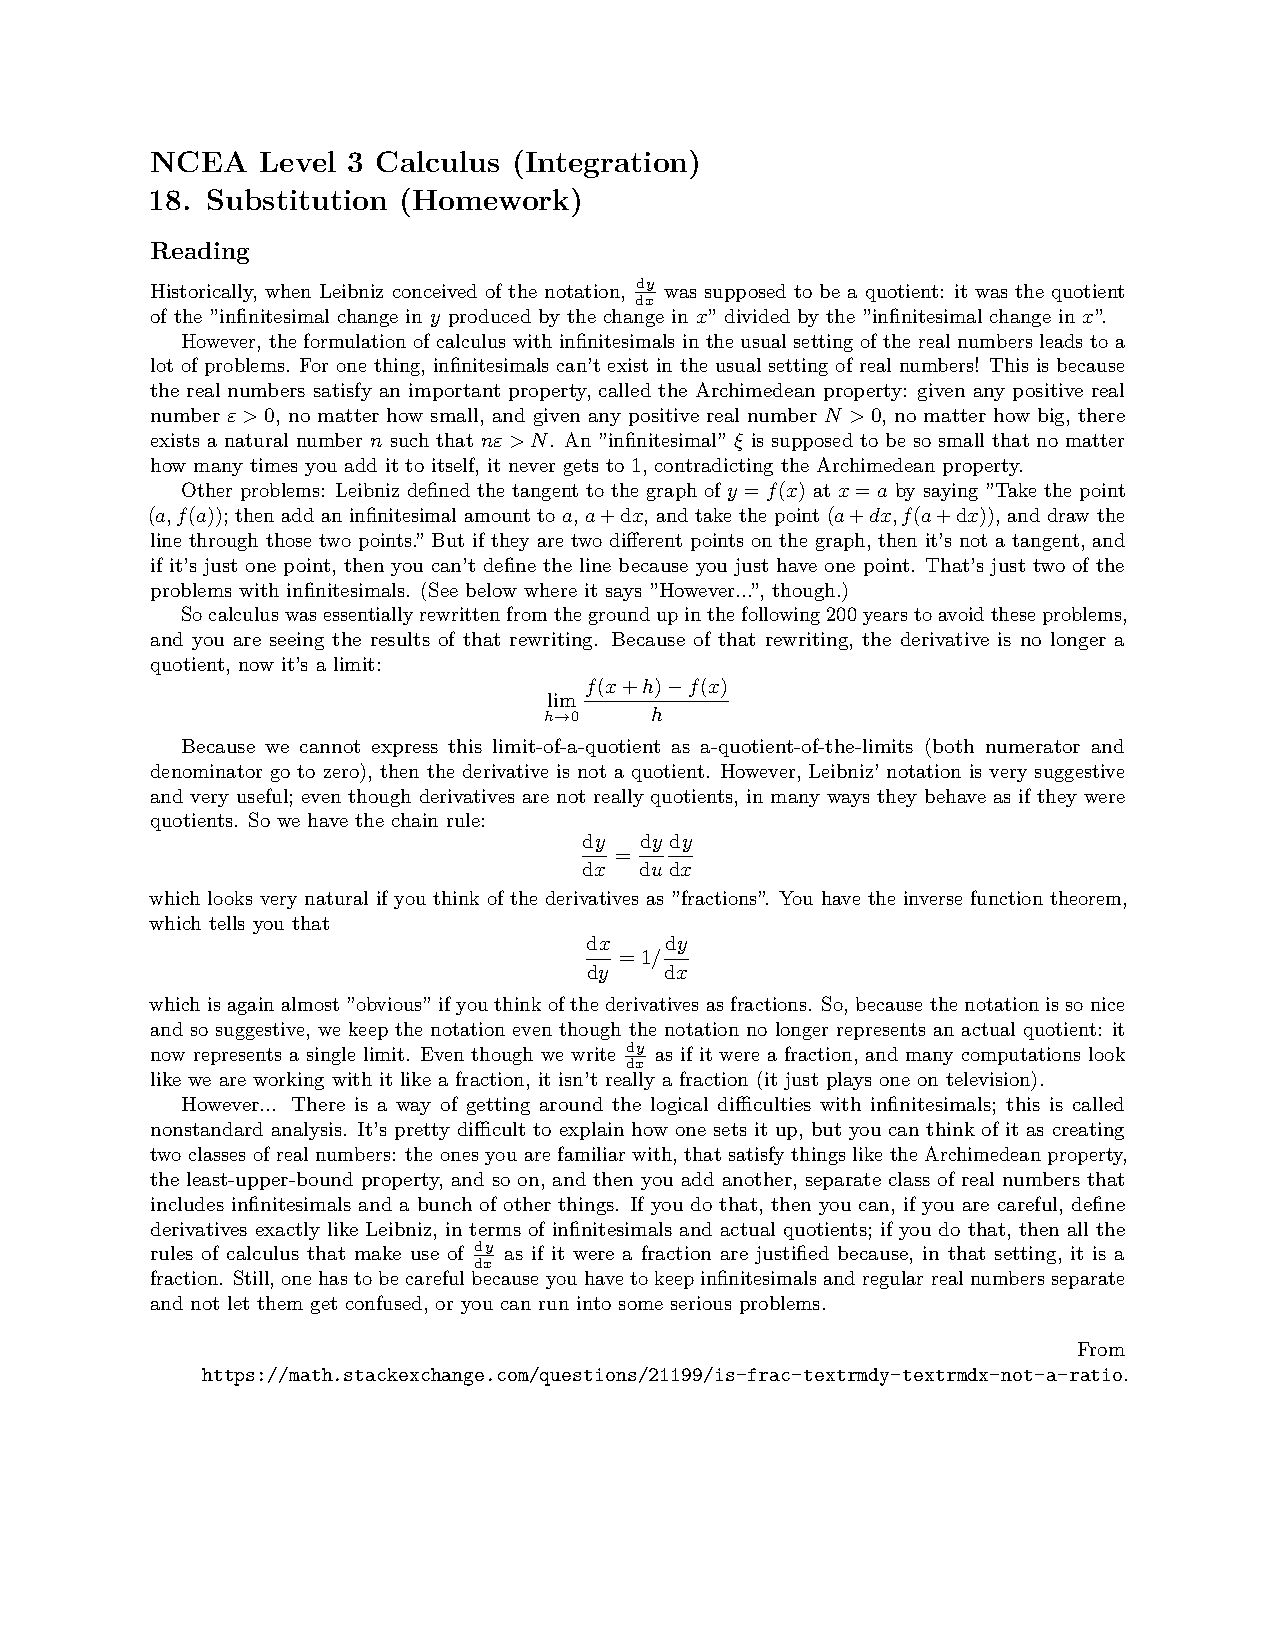
\includepdf[pages={-},pagecommand={}]{18-subsn-hw.pdf}
  \phantomsection\addcontentsline{toc}{section}{19. Differential Equations}
  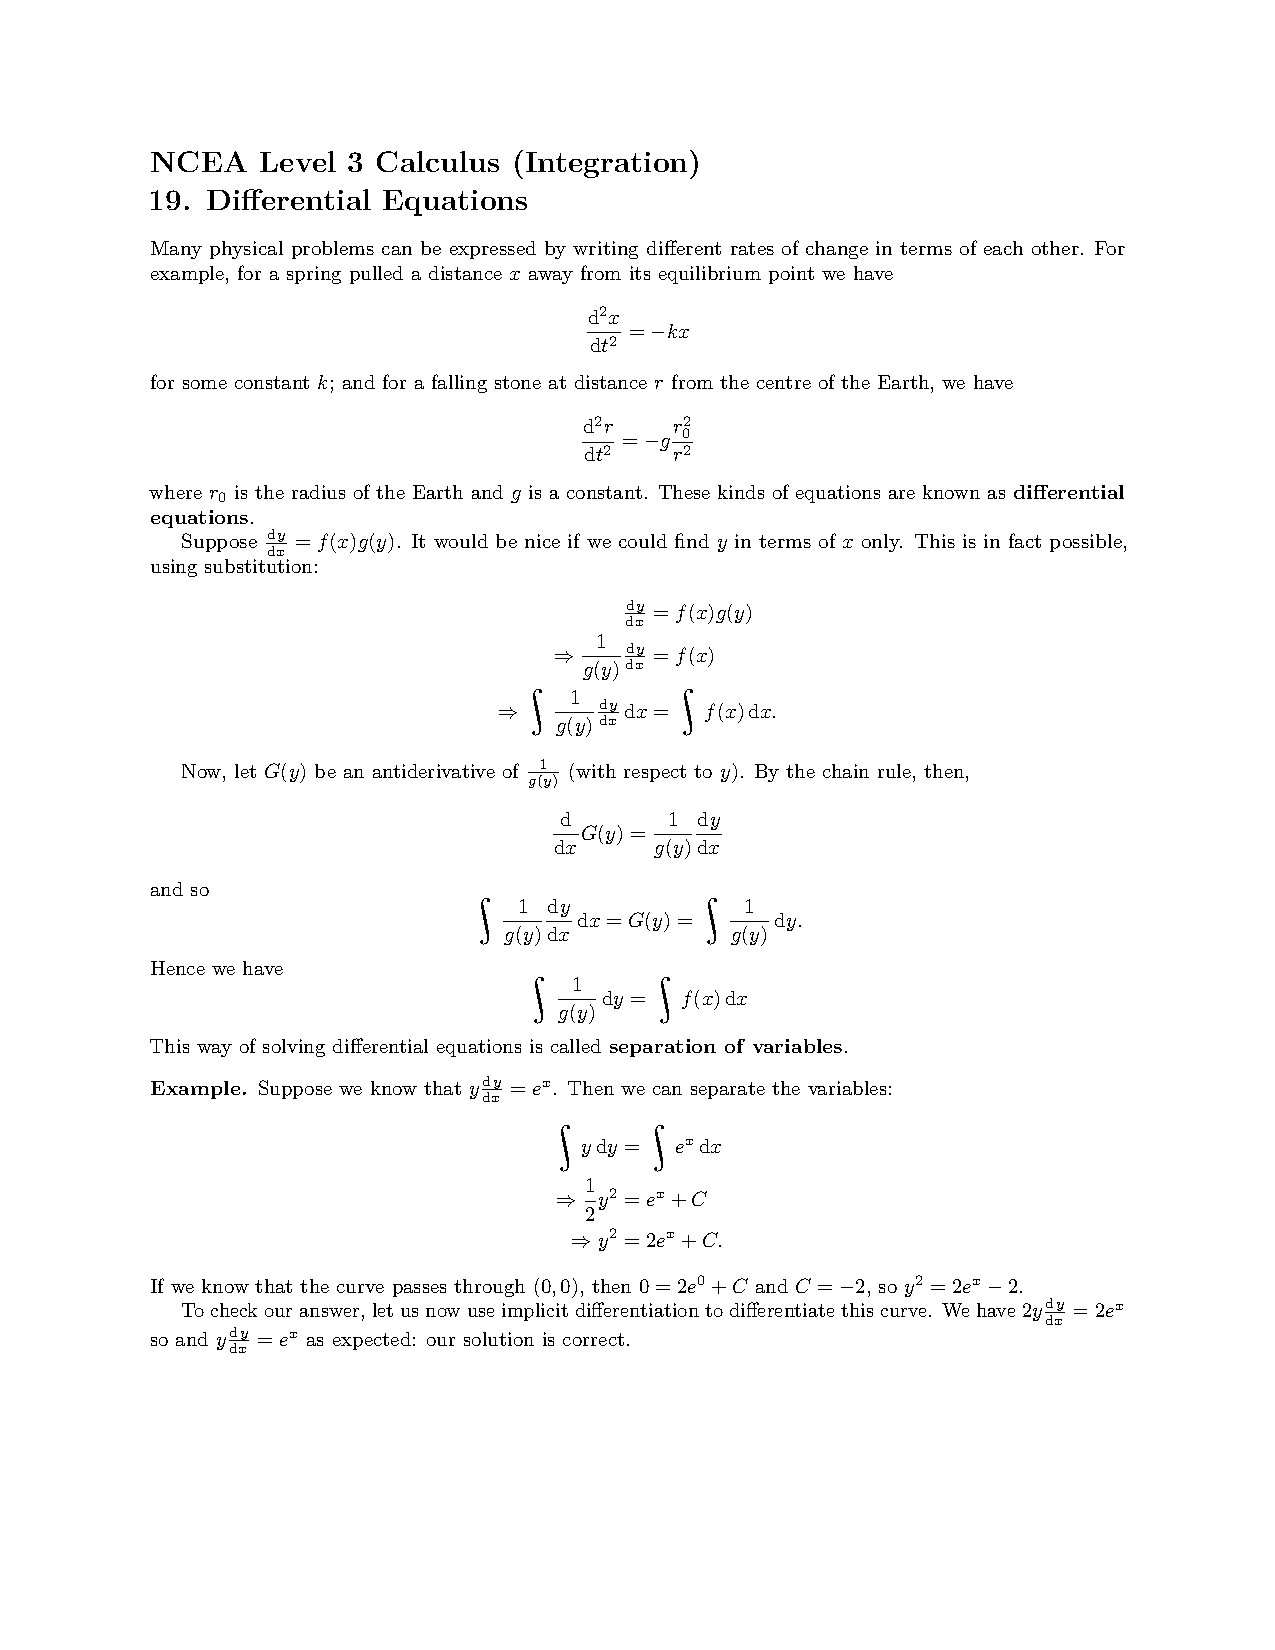
\includepdf[pages={-},pagecommand={}]{19-diffeqs.pdf}
  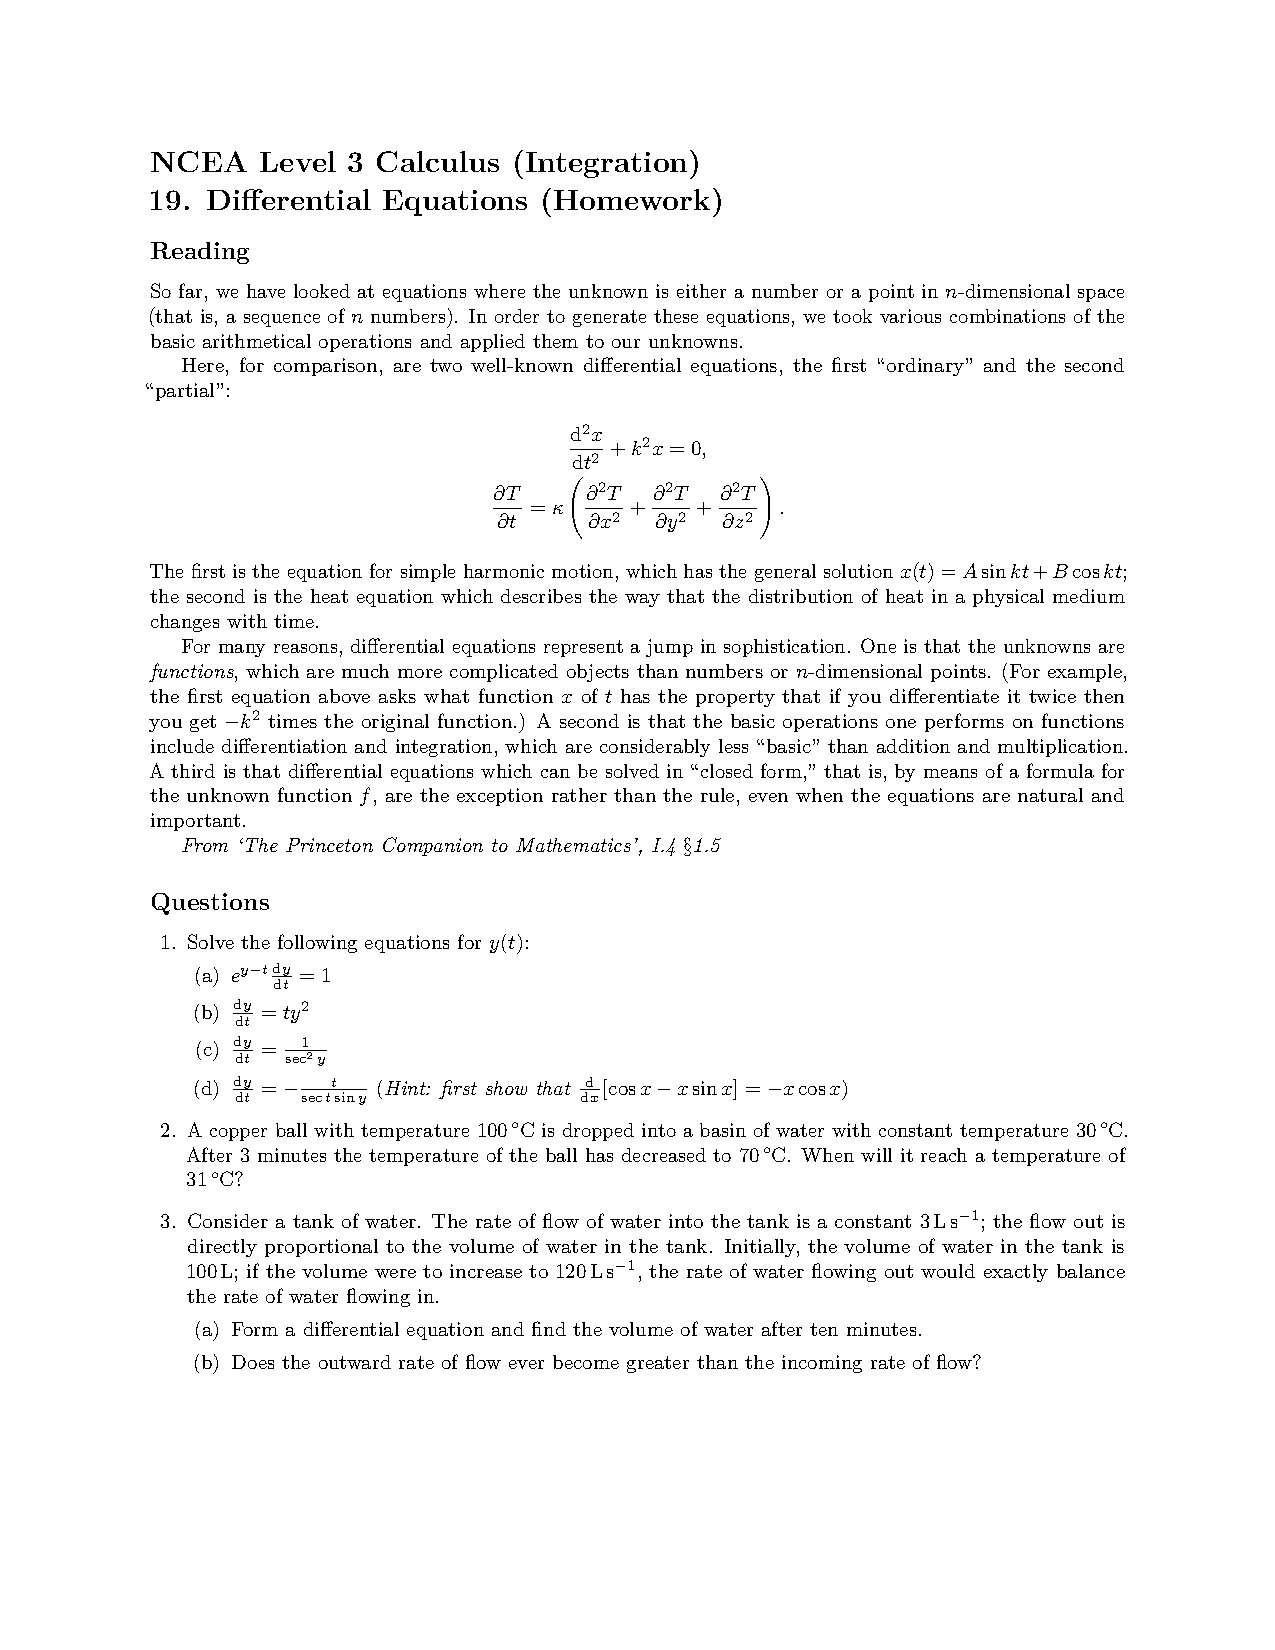
\includepdf[pages={-},pagecommand={}]{19-diffeqs-hw.pdf}
  \phantomsection\addcontentsline{toc}{section}{Integration Assignment}
  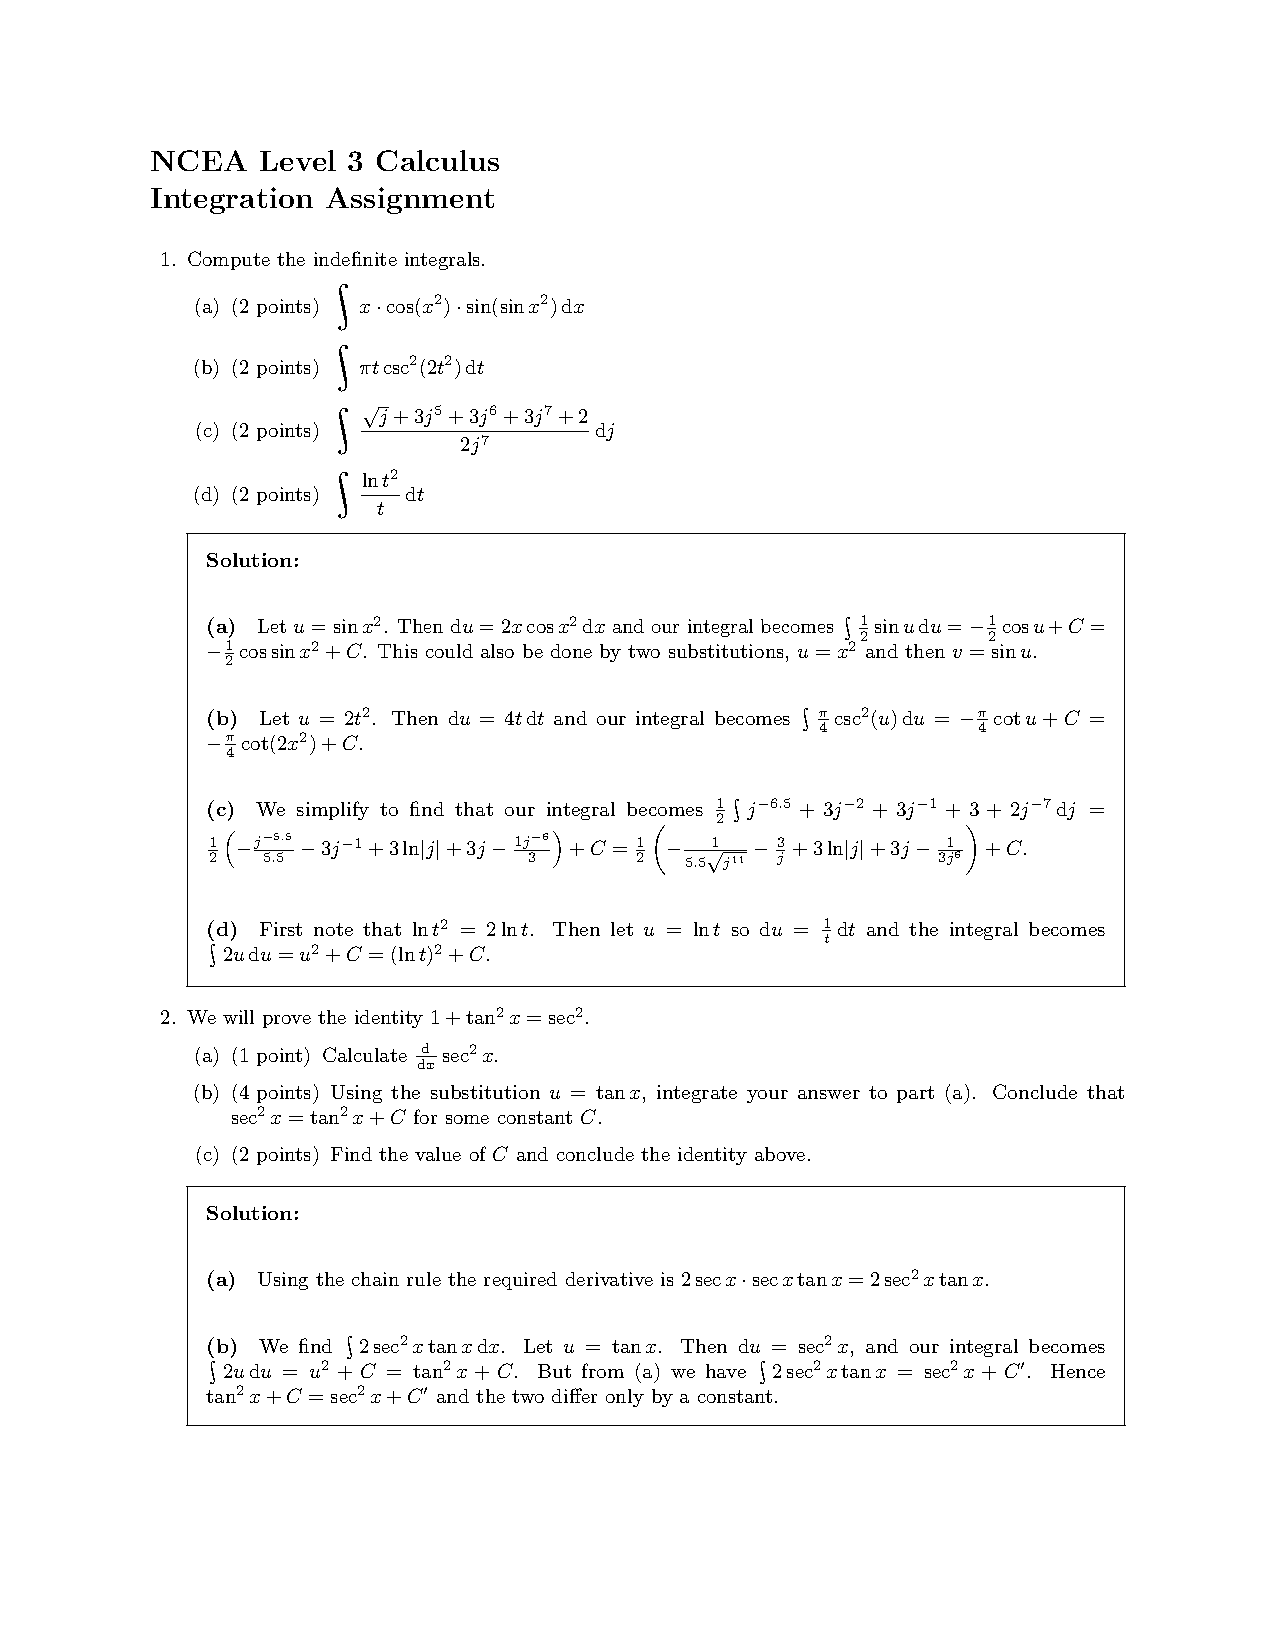
\includepdf[pages={-},pagecommand={}]{asst-integration.pdf}
  \phantomsection\addcontentsline{toc}{section}{20. Partial Fractions}
  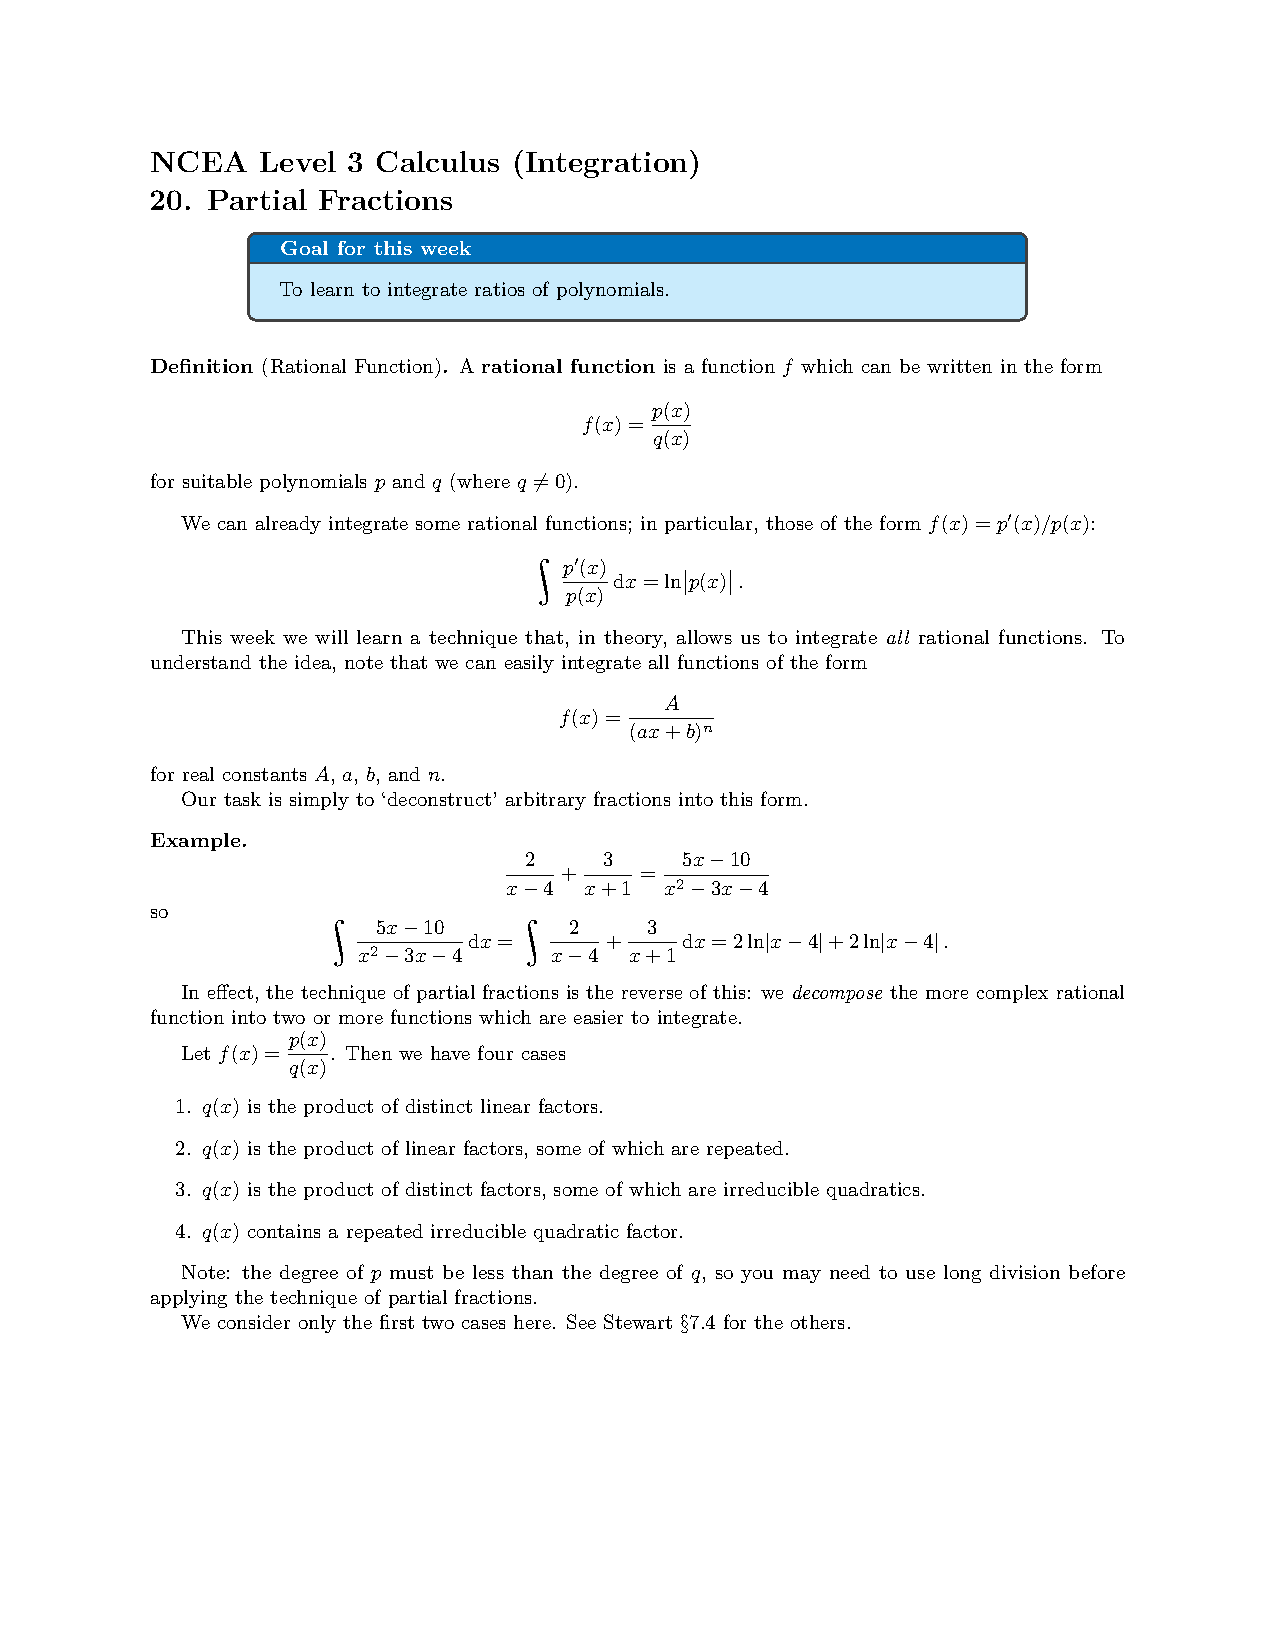
\includepdf[pages={-},pagecommand={}]{20-parfracs.pdf}
  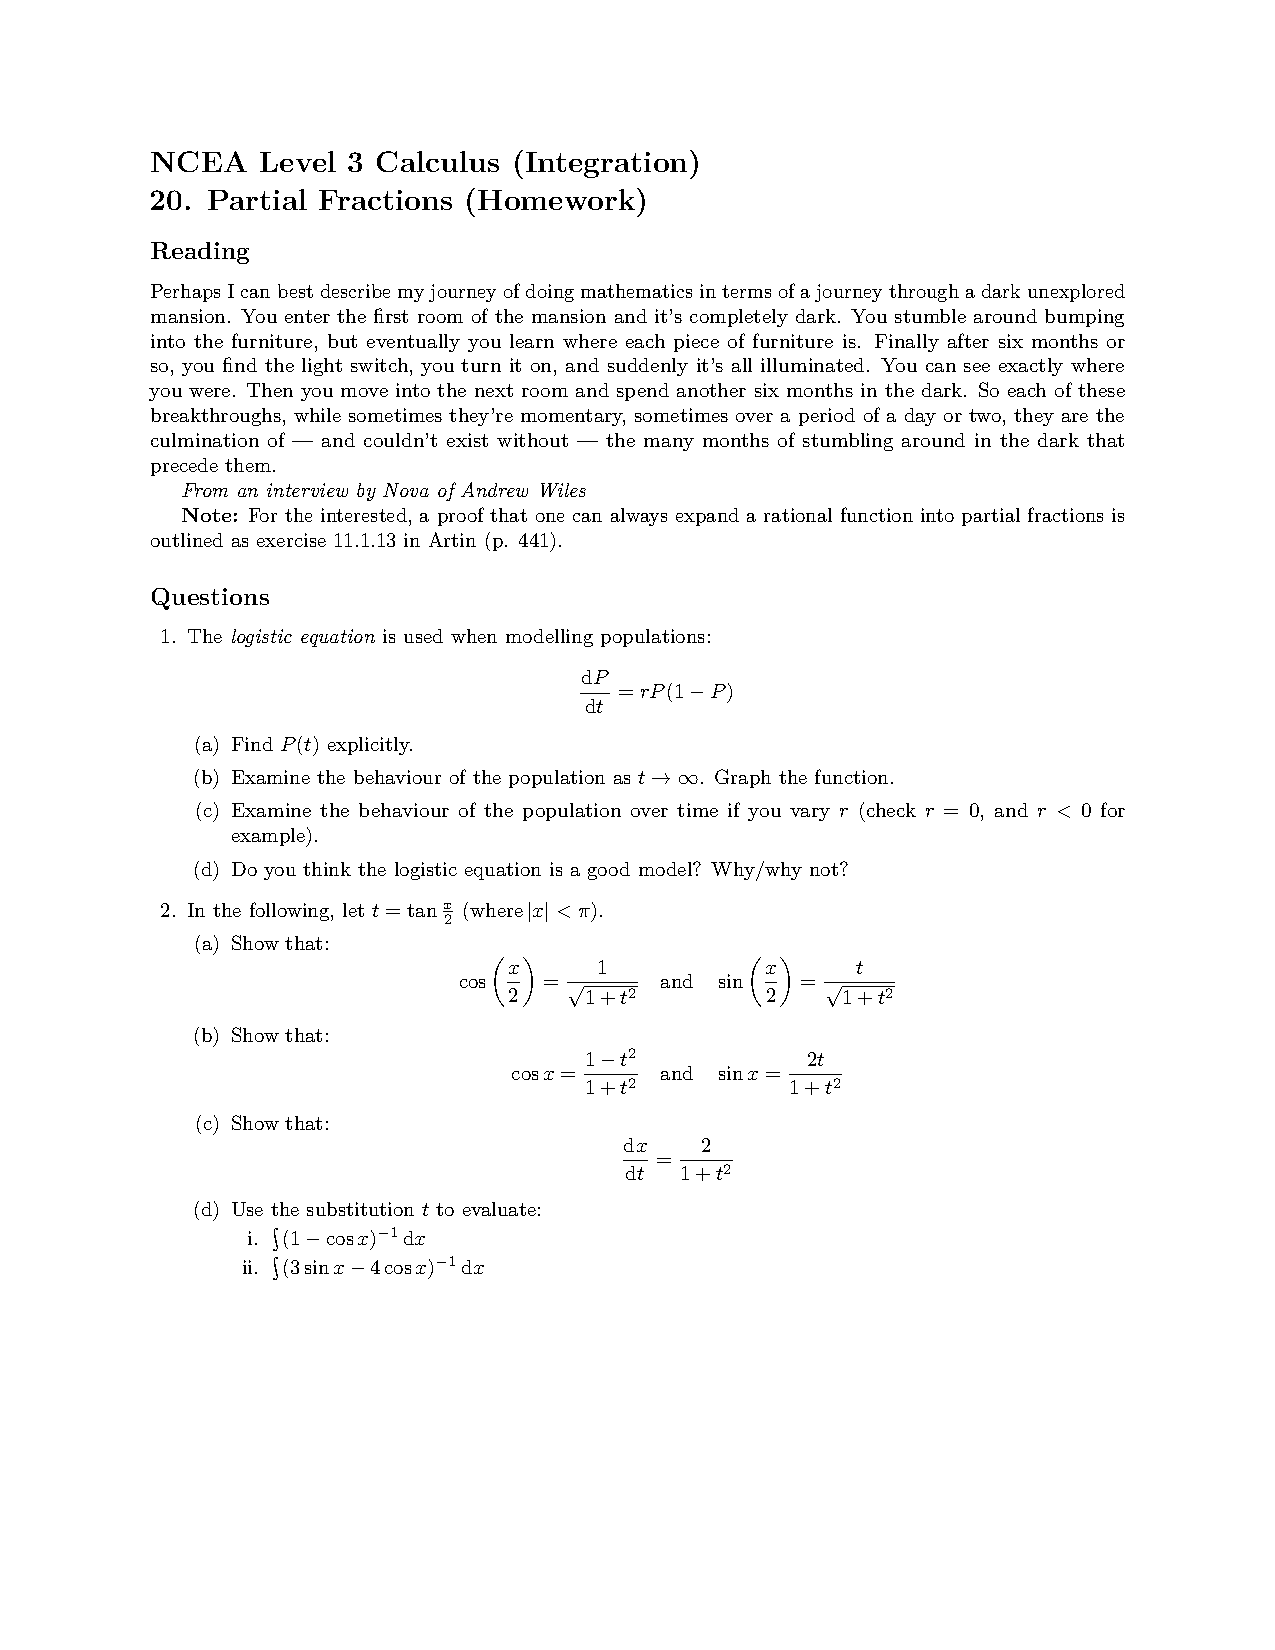
\includepdf[pages={-},pagecommand={}]{20-parfracs-hw.pdf}
  \phantomsection\addcontentsline{toc}{section}{21. Integration by Parts}
  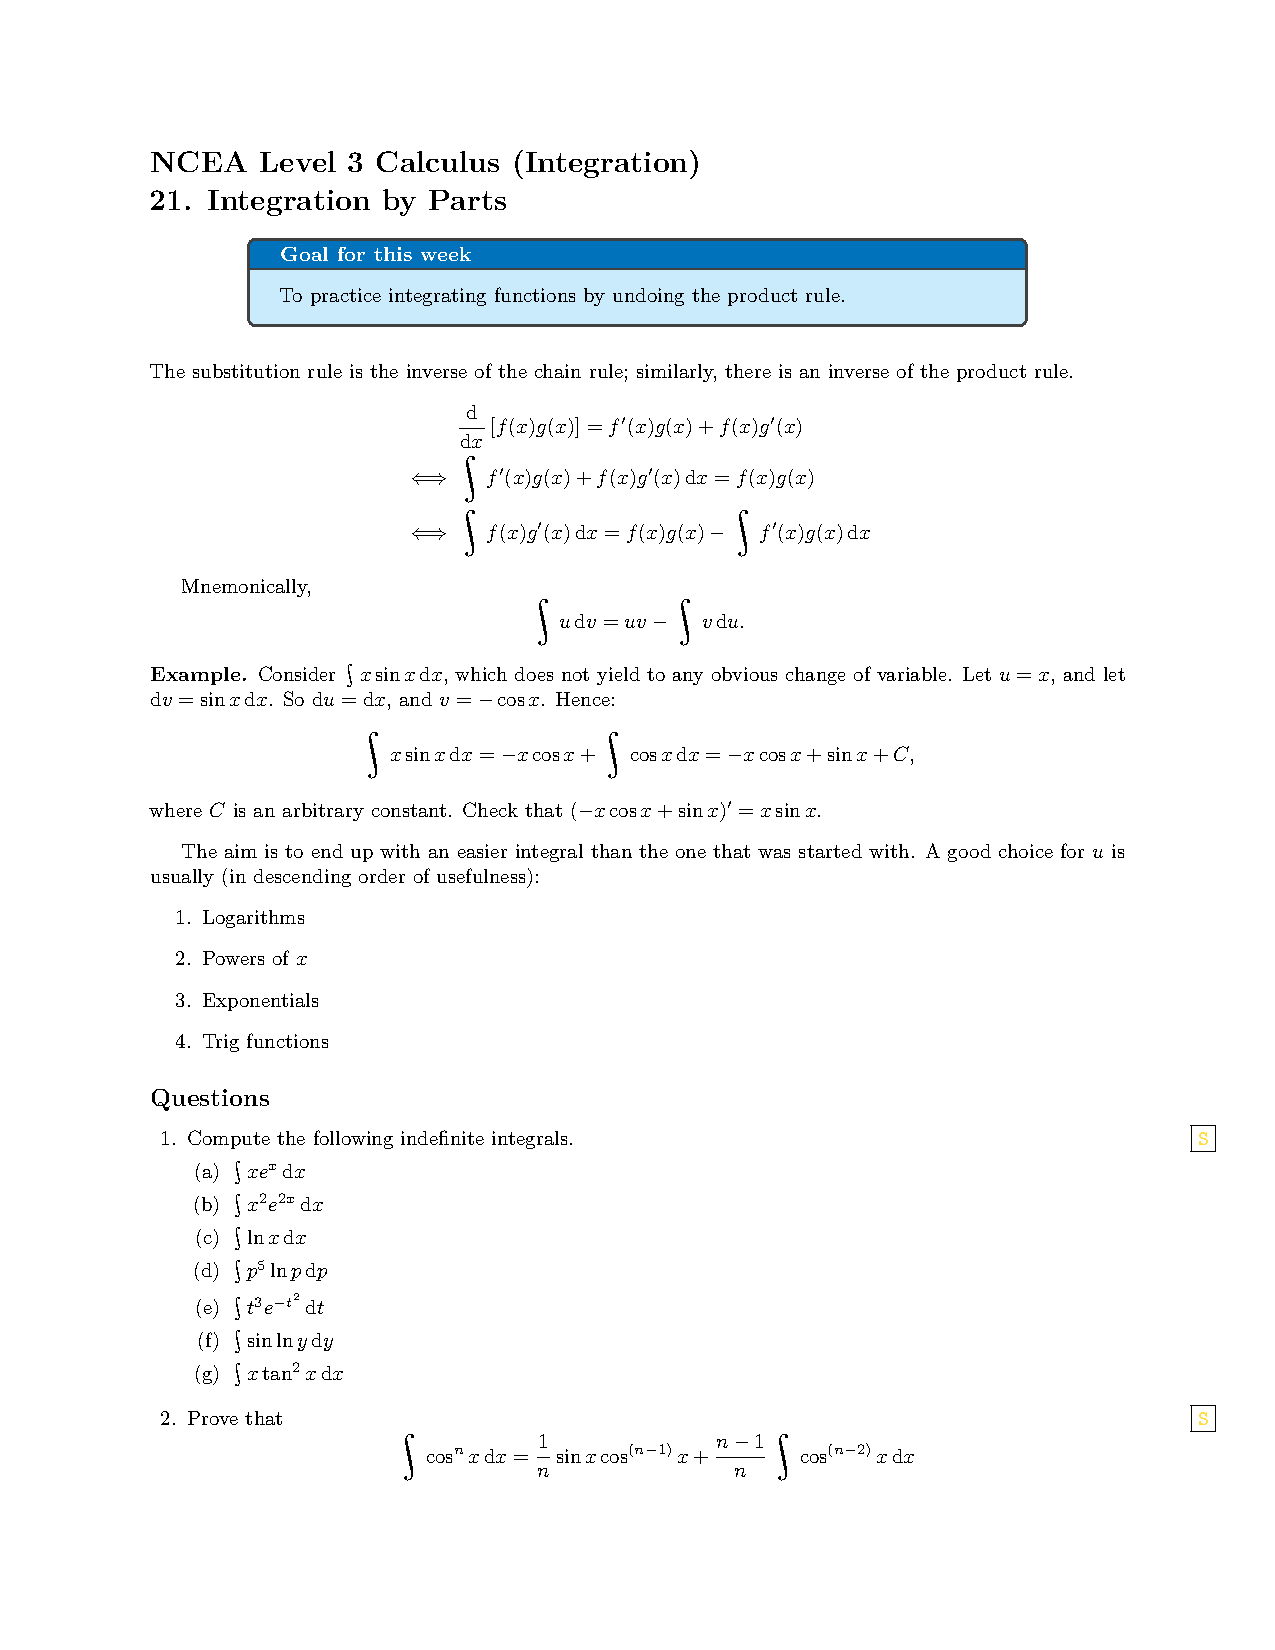
\includepdf[pages={-},pagecommand={}]{21-parts.pdf}
  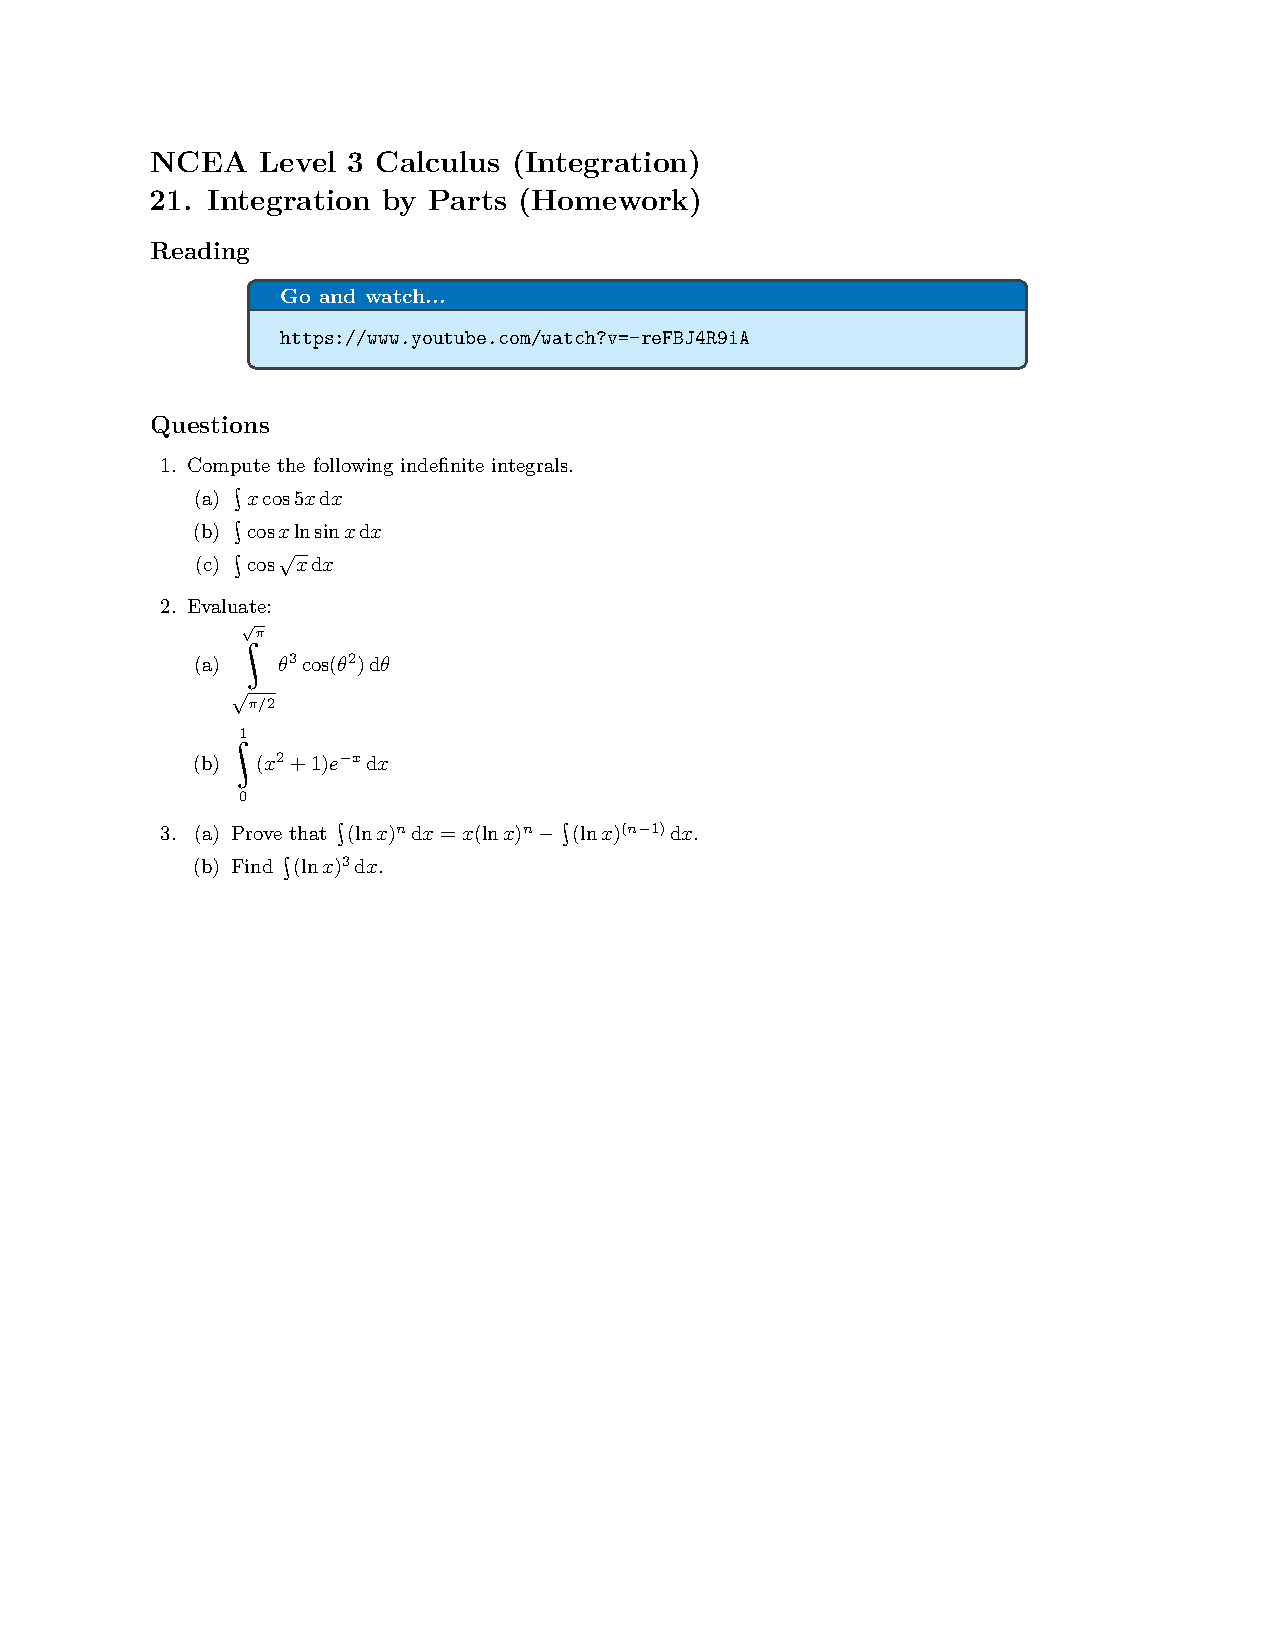
\includepdf[pages={-},pagecommand={}]{21-parts-hw.pdf}
  \phantomsection\addcontentsline{toc}{section}{22. Lengths, Volumes, and Areas}
  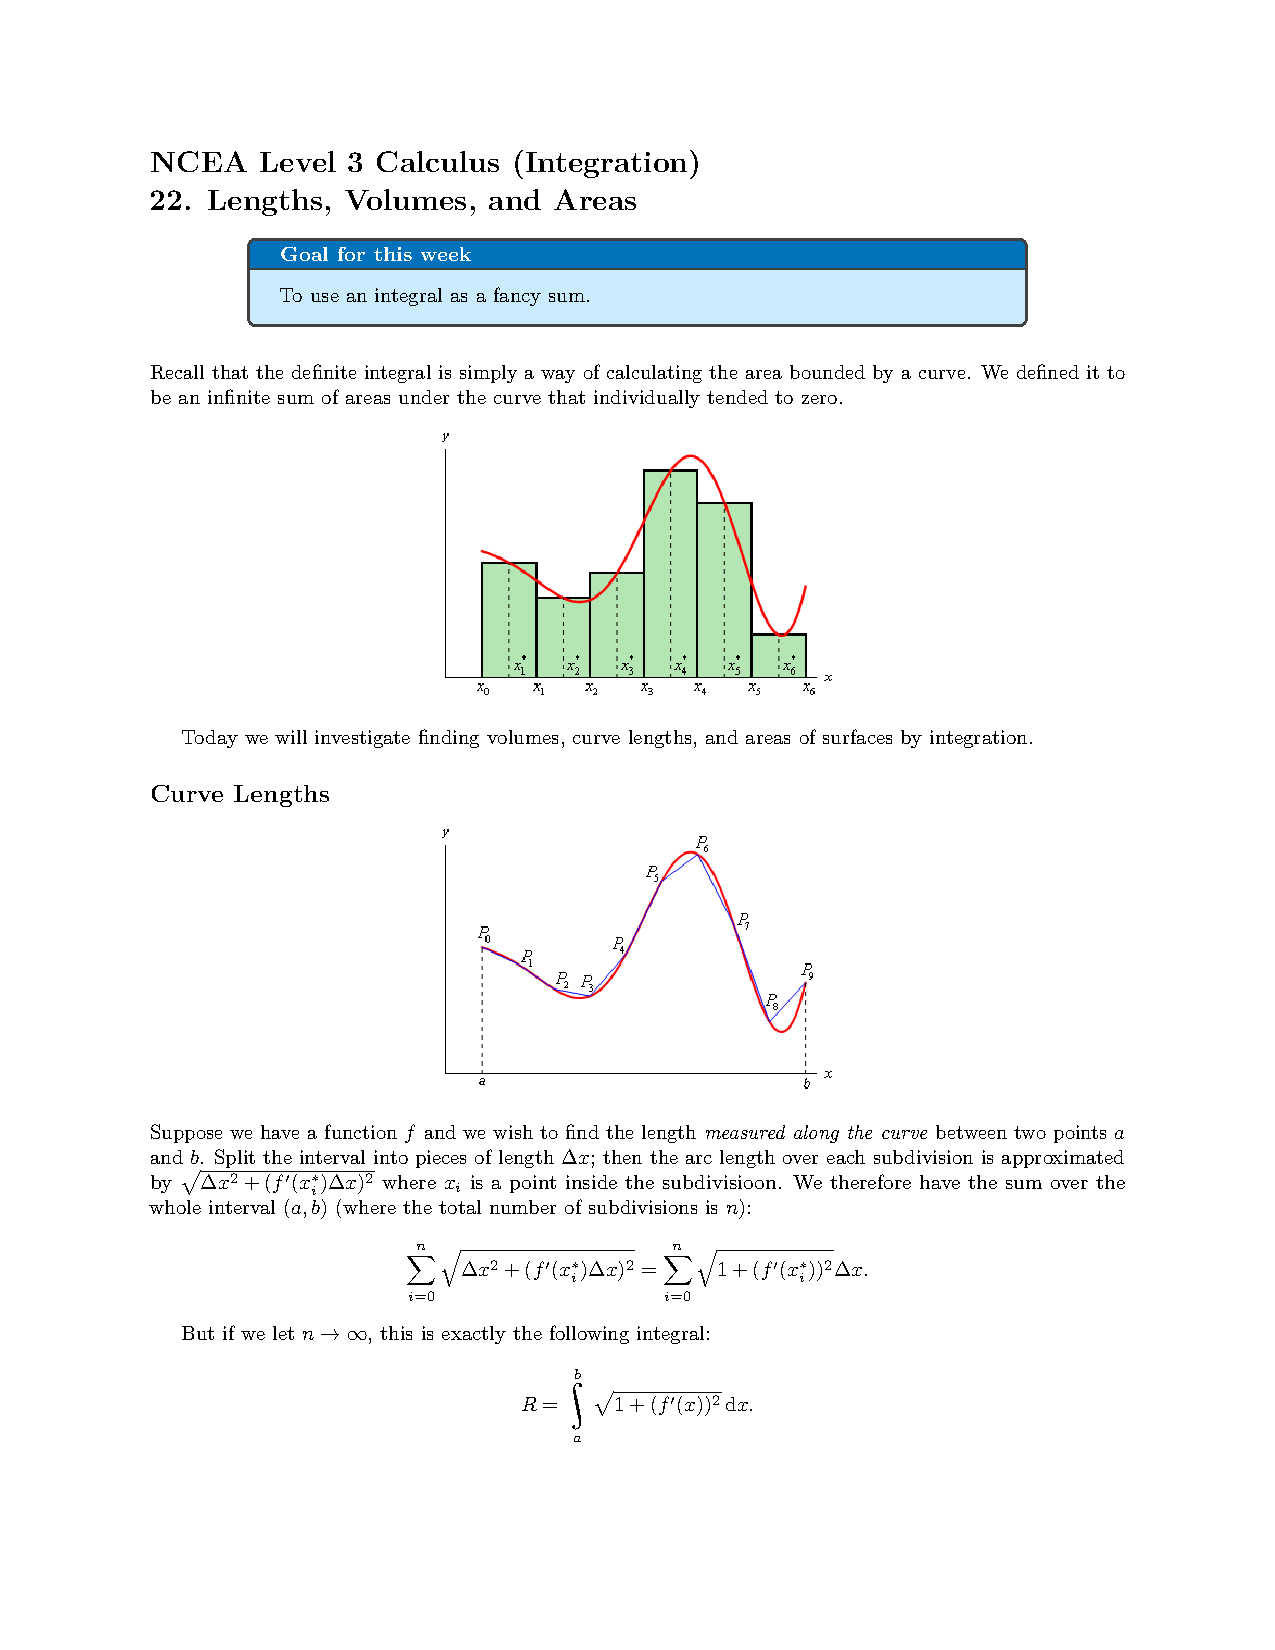
\includepdf[pages={-},pagecommand={}]{22-summing.pdf}
  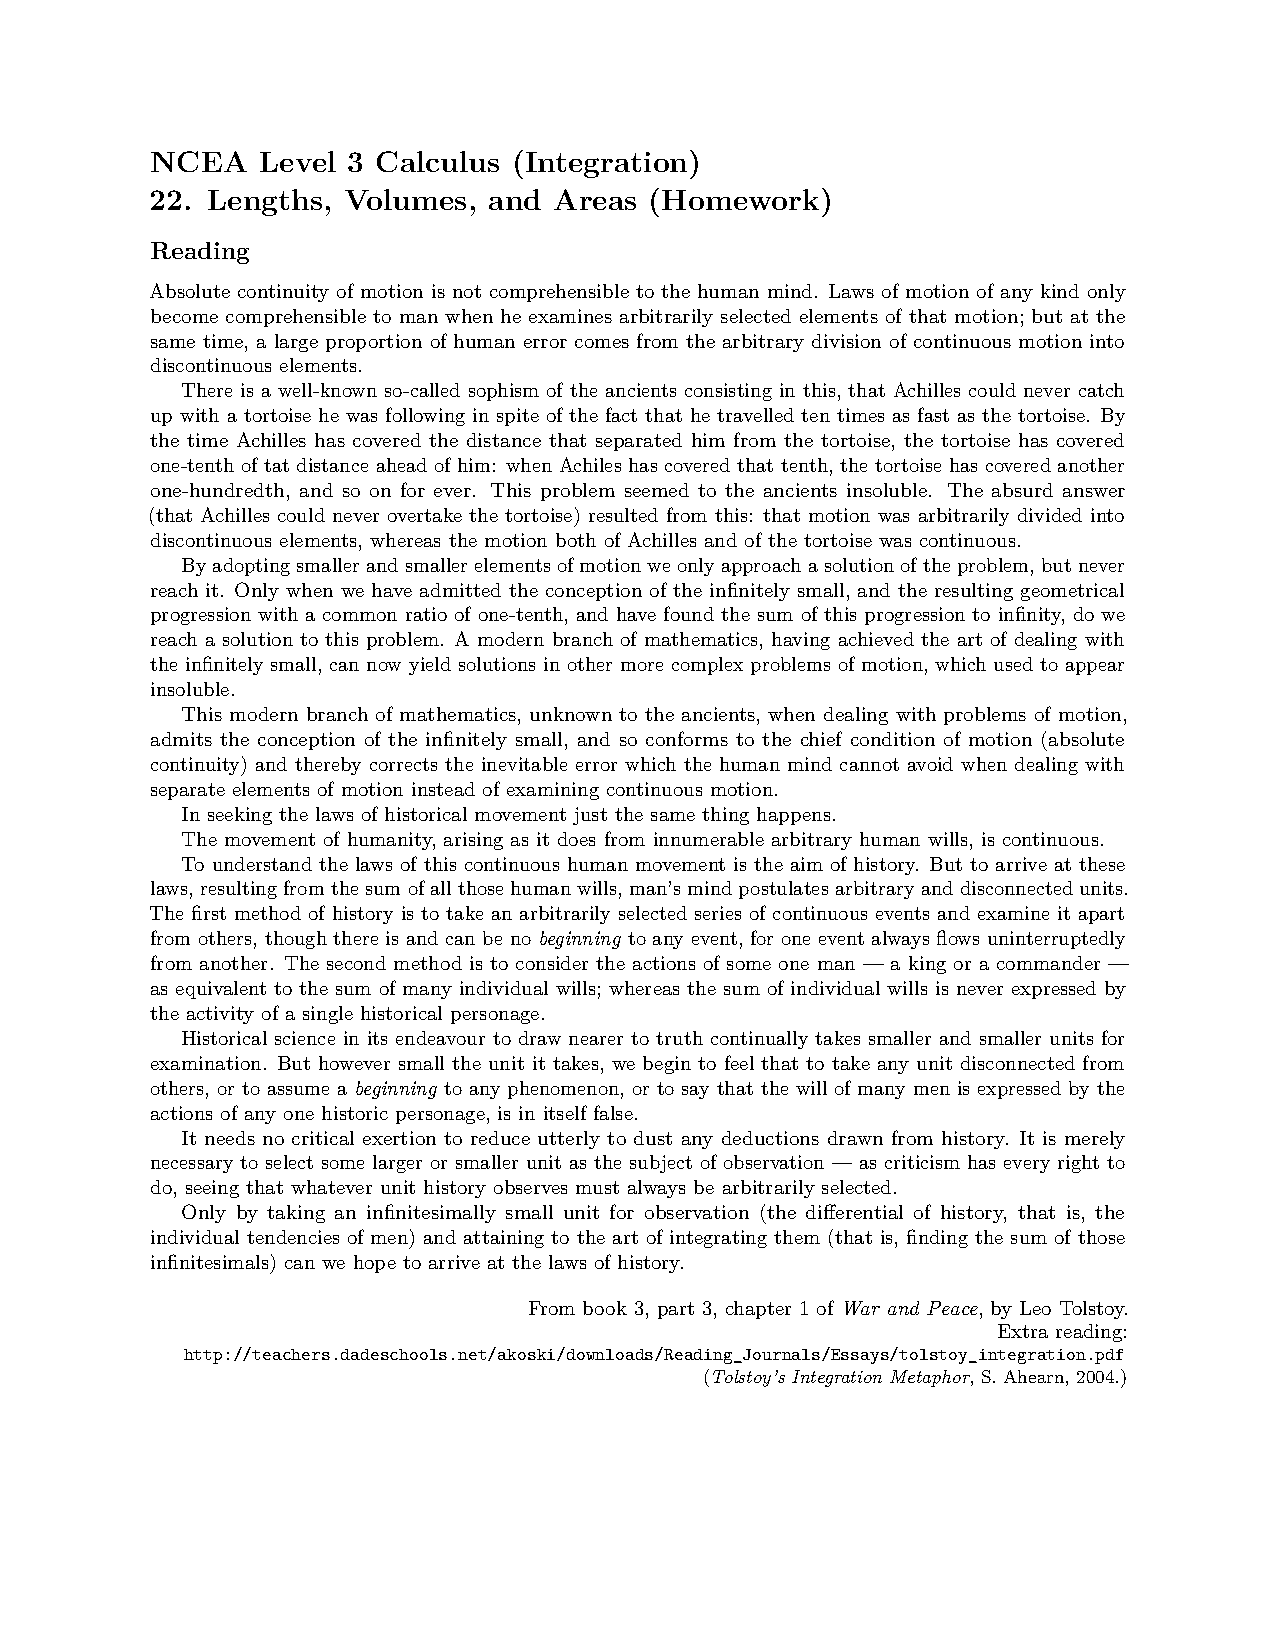
\includepdf[pages={-},pagecommand={}]{22-summing-hw.pdf}
  \phantomsection\addcontentsline{toc}{section}{23. Trigonometric Substitution}
  \includepdf[pages={-},pagecommand={}]{23-trigsubsn.pdf}
  \includepdf[pages={-},pagecommand={}]{23-trigsubsn-hw.pdf}
  \phantomsection\addcontentsline{toc}{section}{24. Kinematics}
  \includepdf[pages={-},pagecommand={}]{24-kinematics.pdf}
  \includepdf[pages={-},pagecommand={}]{24-kinematics-hw.pdf}
  \phantomsection\addcontentsline{toc}{section}{25. Integration Revision}
  \includepdf[pages={-},pagecommand={}]{25-intrev.pdf}
  \includepdf[pages={-},pagecommand={}]{25-intrev-hw.pdf}
  \phantomsection\addcontentsline{toc}{section}{26. More Interesting Problems}
  \includepdf[pages={-},pagecommand={}]{26-moreprobs.pdf}

  \chapter{Additional Material}
  \phantomsection\addcontentsline{toc}{section}{Exam Advice}
  \includepdf[pages={-},pagecommand={}]{EX-examadvice.pdf}
  \phantomsection\addcontentsline{toc}{section}{Solutions to Homeworks}
  \includepdf[pages={-},pagecommand={}]{homework-solutions.pdf}
  \phantomsection\addcontentsline{toc}{section}{NZQA Scholarship Calculus Formulae Booklet}
  \includepdf[pages={-},pagecommand={}]{Scholarship-Calculus-formulae-booklet.pdf}
\end{document}
